\documentclass{amsart}[12pt]

\addtolength{\oddsidemargin}{-.75in}%
\addtolength{\evensidemargin}{-.75in}%
\addtolength{\textwidth}{1.5in}%
\addtolength{\textheight}{1.3in}%
\addtolength{\topmargin}{-.8in}%
\addtolength{\marginparpush}{-.75in}%
%\setlength\parindent{0pt}
%\setlength{\bibsep}{0pt plus 0.3ex}

\usepackage[authoryear]{natbib}
\usepackage[doublespacing]{setspace}
\usepackage{graphicx}
\usepackage{algorithm,algorithmic}
\usepackage{color}
\usepackage{verbatim}
\usepackage{subfigure}
\usepackage{amsfonts}
\usepackage{color}
\usepackage{latexsym,amssymb,amsmath,amsfonts}
%\usepackage{tabularx}
\usepackage{theorem}
\usepackage{verbatim,array,multicol,palatino}
\usepackage{graphics}
\usepackage{fancyhdr}
\usepackage{url}
%\usepackage[all]{xy}

\title{Introduction}
\author{Mark Greenaway}
% include.tex
\newcommand{\Bernoulli}[1]{\text{Bernoulli} \left( #1 \right)}
\newcommand{\mydigamma}[1]{\psi \left( #1 \right)}
%\newcommand{\diag}[1]{\text{diag}\left( #1 \right)}
\newcommand{\tr}[1]{\text{tr}\left( #1 \right)}
\newcommand{\Poisson}[1]{\text{Poisson} \left( #1 \right)}
\def \half {\frac{1}{2}}
\def \R {\mathbb{R}}
\def \vbeta {\vec{\beta}}
\def \vy {\vec{y}}
\def \vmu {\vec{\mu}}
\def \vmuqbeta {\vmu_{q(\vbeta)}}
\def \vmubeta {\vmu_{\vbeta}}
\def \Sigmaqbeta {\Sigma_{q(\vbeta)}}
\def \Sigmabeta {\Sigma_{\vbeta}}
\def \va {\vec{a}}
\def \vtheta {\vec{\theta}}
\def \mX {\vec{X}}

\def\ds{{\displaystyle}}

\def\diag{{\mbox{diag}}}


\usepackage{latexsym,amssymb,amsmath,amsfonts}
%\usepackage{tabularx}
\usepackage{theorem}
\usepackage{verbatim,array,multicol,palatino}
\usepackage{graphicx}
\usepackage{graphics}
\usepackage{fancyhdr}
\usepackage{algorithm,algorithmic}
\usepackage{url}
%\usepackage[all]{xy}



\def\approxdist{\stackrel{{\tiny \mbox{approx.}}}{\sim}}
\def\smhalf{\textstyle{\frac{1}{2}}}
\def\vxnew{\vx_{\mbox{{\tiny new}}}}
\def\bib{\vskip12pt\par\noindent\hangindent=1 true cm\hangafter=1}
\def\jump{\vskip3mm\noindent}
\def\etal{{\em et al.}}
\def\etahat{{\widehat\eta}}
\def\thick#1{\hbox{\rlap{$#1$}\kern0.25pt\rlap{$#1$}\kern0.25pt$#1$}}
\def\smbbeta{{\thick{\scriptstyle{\beta}}}}
\def\smbtheta{{\thick{\scriptstyle{\theta}}}}
\def\smbu{{\thick{\scriptstyle{\rm u}}}}
\def\smbzero{{\thick{\scriptstyle{0}}}}
\def\boxit#1{\begin{center}\fbox{#1}\end{center}}
\def\lboxit#1{\vbox{\hrule\hbox{\vrule\kern6pt
      \vbox{\kern6pt#1\kern6pt}\kern6pt\vrule}\hrule}}
\def\thickboxit#1{\vbox{{\hrule height 1mm}\hbox{{\vrule width 1mm}\kern6pt
          \vbox{\kern6pt#1\kern6pt}\kern6pt{\vrule width 1mm}}
               {\hrule height 1mm}}}


%\sloppy
%\usepackage{geometry}
%\geometry{verbose,a4paper,tmargin=20mm,bmargin=20mm,lmargin=40mm,rmargin=20mm}


%%%%%%%%%%%%%%%%%%%%%%%%%%%%%%%%%%%%%%%%%%%%%%%%%%%%%%%%%%%%%%%%%%%%%%%%%%%%%%%%
%
% Some convenience definitions
%
% \bf      -> vector
% \sf      -> matrix
% \mathcal -> sets or statistical
% \mathbb  -> fields or statistical
%
%%%%%%%%%%%%%%%%%%%%%%%%%%%%%%%%%%%%%%%%%%%%%%%%%%%%%%%%%%%%%%%%%%%%%%%%%%%%%%%%

% Sets or statistical values
\def\sI{{\mathcal I}}                            % Current Index set
\def\sJ{{\mathcal J}}                            % Select Index set
\def\sL{{\mathcal L}}                            % Likelihood
\def\sl{{\ell}}                                  % Log-likelihood
\def\sN{{\mathcal N}}                            
\def\sS{{\mathcal S}}                            
\def\sP{{\mathcal P}}                            
\def\sQ{{\mathcal Q}}                            
\def\sB{{\mathcal B}}                            
\def\sD{{\mathcal D}}                            
\def\sT{{\mathcal T}}
\def\sE{{\mathcal E}}                            
\def\sF{{\mathcal F}}                            
\def\sC{{\mathcal C}}                            
\def\sO{{\mathcal O}}                            
\def\sH{{\mathcal H}} 
\def\sR{{\mathcal R}}                            
\def\sJ{{\mathcal J}}                            
\def\sCP{{\mathcal CP}}                            
\def\sX{{\mathcal X}}                            
\def\sA{{\mathcal A}} 
\def\sZ{{\mathcal Z}}                            
\def\sM{{\mathcal M}}                            
\def\sK{{\mathcal K}}     
\def\sG{{\mathcal G}}                         
\def\sY{{\mathcal Y}}                         
\def\sU{{\mathcal U}}  


\def\sIG{{\mathcal IG}}                            


\def\cD{{\sf D}}
\def\cH{{\sf H}}
\def\cI{{\sf I}}

% Vectors
\def\vectorfontone{\bf}
\def\vectorfonttwo{\boldsymbol}
\def\va{{\vectorfontone a}}                      %
\def\vb{{\vectorfontone b}}                      %
\def\vc{{\vectorfontone c}}                      %
\def\vd{{\vectorfontone d}}                      %
\def\ve{{\vectorfontone e}}                      %
\def\vf{{\vectorfontone f}}                      %
\def\vg{{\vectorfontone g}}                      %
\def\vh{{\vectorfontone h}}                      %
\def\vi{{\vectorfontone i}}                      %
\def\vj{{\vectorfontone j}}                      %
\def\vk{{\vectorfontone k}}                      %
\def\vl{{\vectorfontone l}}                      %
\def\vm{{\vectorfontone m}}                      % number of basis functions
\def\vn{{\vectorfontone n}}                      % number of training samples
\def\vo{{\vectorfontone o}}                      %
\def\vp{{\vectorfontone p}}                      % number of unpenalized coefficients
\def\vq{{\vectorfontone q}}                      % number of penalized coefficients
\def\vr{{\vectorfontone r}}                      %
\def\vs{{\vectorfontone s}}                      %
\def\vt{{\vectorfontone t}}                      %
\def\vu{{\vectorfontone u}}                      % Penalized coefficients
\def\vv{{\vectorfontone v}}                      %
\def\vw{{\vectorfontone w}}                      %
\def\vx{{\vectorfontone x}}                      % Covariates/Predictors
\def\vy{{\vectorfontone y}}                      % Targets/Labels
\def\vz{{\vectorfontone z}}                      %

\def\vone{{\vectorfontone 1}}
\def\vzero{{\vectorfontone 0}}

\def\valpha{{\vectorfonttwo \alpha}}             %
\def\vbeta{{\vectorfonttwo \beta}}               % Unpenalized coefficients
\def\vgamma{{\vectorfonttwo \gamma}}             %
\def\vdelta{{\vectorfonttwo \delta}}             %
\def\vepsilon{{\vectorfonttwo \epsilon}}         %
\def\vvarepsilon{{\vectorfonttwo \varepsilon}}   % Vector of errors
\def\vzeta{{\vectorfonttwo \zeta}}               %
\def\veta{{\vectorfonttwo \eta}}                 % Vector of natural parameters
\def\vtheta{{\vectorfonttwo \theta}}             % Vector of combined coefficients
\def\vvartheta{{\vectorfonttwo \vartheta}}       %
\def\viota{{\vectorfonttwo \iota}}               %
\def\vkappa{{\vectorfonttwo \kappa}}             %
\def\vlambda{{\vectorfonttwo \lambda}}           % Vector of smoothing parameters
\def\vmu{{\vectorfonttwo \mu}}                   % Vector of means
\def\vnu{{\vectorfonttwo \nu}}                   %
\def\vxi{{\vectorfonttwo \xi}}                   %
\def\vpi{{\vectorfonttwo \pi}}                   %
\def\vvarpi{{\vectorfonttwo \varpi}}             %
\def\vrho{{\vectorfonttwo \rho}}                 %
\def\vvarrho{{\vectorfonttwo \varrho}}           %
\def\vsigma{{\vectorfonttwo \sigma}}             %
\def\vvarsigma{{\vectorfonttwo \varsigma}}       %
\def\vtau{{\vectorfonttwo \tau}}                 %
\def\vupsilon{{\vectorfonttwo \upsilon}}         %
\def\vphi{{\vectorfonttwo \phi}}                 %
\def\vvarphi{{\vectorfonttwo \varphi}}           %
\def\vchi{{\vectorfonttwo \chi}}                 %
\def\vpsi{{\vectorfonttwo \psi}}                 %
\def\vomega{{\vectorfonttwo \omega}}             %


% Matrices
%\def\matrixfontone{\sf}
%\def\matrixfonttwo{\sf}
\def\matrixfontone{\bf}
\def\matrixfonttwo{\boldsymbol}
\def\mA{{\matrixfontone A}}                      %
\def\mB{{\matrixfontone B}}                      %
\def\mC{{\matrixfontone C}}                      % Combined Design Matrix
\def\mD{{\matrixfontone D}}                      % Penalty Matrix for \vu_J
\def\mE{{\matrixfontone E}}                      %
\def\mF{{\matrixfontone F}}                      %
\def\mG{{\matrixfontone G}}                      % Penalty Matrix for \vu
\def\mH{{\matrixfontone H}}                      %
\def\mI{{\matrixfontone I}}                      % Identity Matrix
\def\mJ{{\matrixfontone J}}                      %
\def\mK{{\matrixfontone K}}                      %
\def\mL{{\matrixfontone L}}                      % Lower bound
\def\mM{{\matrixfontone M}}                      %
\def\mN{{\matrixfontone N}}                      %
\def\mO{{\matrixfontone O}}                      %
\def\mP{{\matrixfontone P}}                      %
\def\mQ{{\matrixfontone Q}}                      %
\def\mR{{\matrixfontone R}}                      %
\def\mS{{\matrixfontone S}}                      %
\def\mT{{\matrixfontone T}}                      %
\def\mU{{\matrixfontone U}}                      % Upper bound
\def\mV{{\matrixfontone V}}                      %
\def\mW{{\matrixfontone W}}                      % Variance Matrix i.e. diag(b'')
\def\mX{{\matrixfontone X}}                      % Unpenalized Design Matrix/Nullspace Matrix
\def\mY{{\matrixfontone Y}}                      %
\def\mZ{{\matrixfontone Z}}                      % Penalized Design Matrix/Kernel Space Matrix

\def\mGamma{{\matrixfonttwo \Gamma}}             %
\def\mDelta{{\matrixfonttwo \Delta}}             %
\def\mTheta{{\matrixfonttwo \Theta}}             %
\def\mLambda{{\matrixfonttwo \Lambda}}           % Penalty Matrix for \vnu
\def\mXi{{\matrixfonttwo \Xi}}                   %
\def\mPi{{\matrixfonttwo \Pi}}                   %
\def\mSigma{{\matrixfonttwo \Sigma}}             %
\def\mUpsilon{{\matrixfonttwo \Upsilon}}         %
\def\mPhi{{\matrixfonttwo \Phi}}                 %
\def\mOmega{{\matrixfonttwo \Omega}}             %
\def\mPsi{{\matrixfonttwo \Psi}}                 %

\def\mone{{\matrixfontone 1}}
\def\mzero{{\matrixfontone 0}}

% Fields or Statistical
\def\bE{{\mathbb E}}                             % Expectation
\def\bP{{\mathbb P}}                             % Probability
\def\bR{{\mathbb R}}                             % Reals
\def\bI{{\mathbb I}}                             % Reals
\def\bV{{\mathbb V}}                             % Reals

\def\vX{{\vectorfontone X}}                      % Targets/Labels
\def\vY{{\vectorfontone Y}}                      % Targets/Labels
\def\vZ{{\vectorfontone Z}}                      %

% Other
\def\etal{{\em et al.}}
\def\ds{\displaystyle}
\def\d{\partial}
\def\diag{\text{diag}}
%\def\span{\text{span}}
\def\blockdiag{\text{blockdiag}}
\def\tr{\text{tr}}
\def\RSS{\text{RSS}}
\def\df{\text{df}}
\def\GCV{\text{GCV}}
\def\AIC{\text{AIC}}
\def\MLC{\text{MLC}}
\def\mAIC{\text{mAIC}}
\def\cAIC{\text{cAIC}}
\def\rank{\text{rank}}
\def\MASE{\text{MASE}}
\def\SMSE{\text{SASE}}
\def\sign{\text{sign}}
\def\card{\text{card}}
\def\notexp{\text{notexp}}
\def\ASE{\text{ASE}}
\def\ML{\text{ML}}
\def\nullity{\text{nullity}}

\def\logexpit{\text{logexpit}}
\def\logit{\mbox{logit}}
\def\dg{\mbox{dg}}

\def\Bern{\mbox{Bernoulli}}
\def\sBernoulli{\mbox{Bernoulli}}
\def\sGamma{\mbox{Gamma}}
\def\sInvN{\mbox{Inv}\sN}
\def\sNegBin{\sN\sB}

\def\dGamma{\mbox{Gamma}}
\def\dInvGam{\mbox{Inv}\Gamma}

\def\Cov{\mbox{Cov}}
\def\Mgf{\mbox{Mgf}}

\def\mis{{mis}} 
\def\obs{{obs}}

\def\argmax{\operatornamewithlimits{\text{argmax}}}
\def\argmin{\operatornamewithlimits{\text{argmin}}}
\def\argsup{\operatornamewithlimits{\text{argsup}}}
\def\arginf{\operatornamewithlimits{\text{arginf}}}


\def\minimize{\operatornamewithlimits{\text{minimize}}}
\def\maximize{\operatornamewithlimits{\text{maximize}}}
\def\suchthat{\text{such that}}


\def\relstack#1#2{\mathop{#1}\limits_{#2}}
\def\sfrac#1#2{{\textstyle{\frac{#1}{#2}}}}


\def\comment#1{
\vspace{0.5cm}
\noindent \begin{tabular}{|p{14cm}|}  
\hline #1 \\ 
\hline 
\end{tabular}
\vspace{0.5cm}
}


\def\mytext#1{\begin{tabular}{p{13cm}}#1\end{tabular}}
\def\mytextB#1{\begin{tabular}{p{7.5cm}}#1\end{tabular}}
\def\mytextC#1{\begin{tabular}{p{12cm}}#1\end{tabular}}

\def\jump{\vskip3mm\noindent}

\def\KL{\text{KL}}
\def\N{\text{N}}
\def\Var{\text{Var}}

\def \E {\mathbb{E}}
\def \BigO {\text{O}}
\def \IG {\text{IG}}
\def \Beta {\text{Beta}}



\usepackage[doublespacing]{setspace}

% include.tex
\newcommand{\Bernoulli}[1]{\text{Bernoulli} \left( #1 \right)}
\newcommand{\mydigamma}[1]{\psi \left( #1 \right)}
%\newcommand{\diag}[1]{\text{diag}\left( #1 \right)}
\newcommand{\tr}[1]{\text{tr}\left( #1 \right)}
\newcommand{\Poisson}[1]{\text{Poisson} \left( #1 \right)}
\def \half {\frac{1}{2}}
\def \R {\mathbb{R}}
\def \vbeta {\vec{\beta}}
\def \vy {\vec{y}}
\def \vmu {\vec{\mu}}
\def \vmuqbeta {\vmu_{q(\vbeta)}}
\def \vmubeta {\vmu_{\vbeta}}
\def \Sigmaqbeta {\Sigma_{q(\vbeta)}}
\def \Sigmabeta {\Sigma_{\vbeta}}
\def \va {\vec{a}}
\def \vtheta {\vec{\theta}}
\def \mX {\vec{X}}

\def\ds{{\displaystyle}}

\def\diag{{\mbox{diag}}}


\usepackage{latexsym,amssymb,amsmath,amsfonts}
%\usepackage{tabularx}
\usepackage{theorem}
\usepackage{verbatim,array,multicol,palatino}
\usepackage{graphicx}
\usepackage{graphics}
\usepackage{fancyhdr}
\usepackage{algorithm,algorithmic}
\usepackage{url}
%\usepackage[all]{xy}



\def\approxdist{\stackrel{{\tiny \mbox{approx.}}}{\sim}}
\def\smhalf{\textstyle{\frac{1}{2}}}
\def\vxnew{\vx_{\mbox{{\tiny new}}}}
\def\bib{\vskip12pt\par\noindent\hangindent=1 true cm\hangafter=1}
\def\jump{\vskip3mm\noindent}
\def\etal{{\em et al.}}
\def\etahat{{\widehat\eta}}
\def\thick#1{\hbox{\rlap{$#1$}\kern0.25pt\rlap{$#1$}\kern0.25pt$#1$}}
\def\smbbeta{{\thick{\scriptstyle{\beta}}}}
\def\smbtheta{{\thick{\scriptstyle{\theta}}}}
\def\smbu{{\thick{\scriptstyle{\rm u}}}}
\def\smbzero{{\thick{\scriptstyle{0}}}}
\def\boxit#1{\begin{center}\fbox{#1}\end{center}}
\def\lboxit#1{\vbox{\hrule\hbox{\vrule\kern6pt
      \vbox{\kern6pt#1\kern6pt}\kern6pt\vrule}\hrule}}
\def\thickboxit#1{\vbox{{\hrule height 1mm}\hbox{{\vrule width 1mm}\kern6pt
          \vbox{\kern6pt#1\kern6pt}\kern6pt{\vrule width 1mm}}
               {\hrule height 1mm}}}


%\sloppy
%\usepackage{geometry}
%\geometry{verbose,a4paper,tmargin=20mm,bmargin=20mm,lmargin=40mm,rmargin=20mm}


%%%%%%%%%%%%%%%%%%%%%%%%%%%%%%%%%%%%%%%%%%%%%%%%%%%%%%%%%%%%%%%%%%%%%%%%%%%%%%%%
%
% Some convenience definitions
%
% \bf      -> vector
% \sf      -> matrix
% \mathcal -> sets or statistical
% \mathbb  -> fields or statistical
%
%%%%%%%%%%%%%%%%%%%%%%%%%%%%%%%%%%%%%%%%%%%%%%%%%%%%%%%%%%%%%%%%%%%%%%%%%%%%%%%%

% Sets or statistical values
\def\sI{{\mathcal I}}                            % Current Index set
\def\sJ{{\mathcal J}}                            % Select Index set
\def\sL{{\mathcal L}}                            % Likelihood
\def\sl{{\ell}}                                  % Log-likelihood
\def\sN{{\mathcal N}}                            
\def\sS{{\mathcal S}}                            
\def\sP{{\mathcal P}}                            
\def\sQ{{\mathcal Q}}                            
\def\sB{{\mathcal B}}                            
\def\sD{{\mathcal D}}                            
\def\sT{{\mathcal T}}
\def\sE{{\mathcal E}}                            
\def\sF{{\mathcal F}}                            
\def\sC{{\mathcal C}}                            
\def\sO{{\mathcal O}}                            
\def\sH{{\mathcal H}} 
\def\sR{{\mathcal R}}                            
\def\sJ{{\mathcal J}}                            
\def\sCP{{\mathcal CP}}                            
\def\sX{{\mathcal X}}                            
\def\sA{{\mathcal A}} 
\def\sZ{{\mathcal Z}}                            
\def\sM{{\mathcal M}}                            
\def\sK{{\mathcal K}}     
\def\sG{{\mathcal G}}                         
\def\sY{{\mathcal Y}}                         
\def\sU{{\mathcal U}}  


\def\sIG{{\mathcal IG}}                            


\def\cD{{\sf D}}
\def\cH{{\sf H}}
\def\cI{{\sf I}}

% Vectors
\def\vectorfontone{\bf}
\def\vectorfonttwo{\boldsymbol}
\def\va{{\vectorfontone a}}                      %
\def\vb{{\vectorfontone b}}                      %
\def\vc{{\vectorfontone c}}                      %
\def\vd{{\vectorfontone d}}                      %
\def\ve{{\vectorfontone e}}                      %
\def\vf{{\vectorfontone f}}                      %
\def\vg{{\vectorfontone g}}                      %
\def\vh{{\vectorfontone h}}                      %
\def\vi{{\vectorfontone i}}                      %
\def\vj{{\vectorfontone j}}                      %
\def\vk{{\vectorfontone k}}                      %
\def\vl{{\vectorfontone l}}                      %
\def\vm{{\vectorfontone m}}                      % number of basis functions
\def\vn{{\vectorfontone n}}                      % number of training samples
\def\vo{{\vectorfontone o}}                      %
\def\vp{{\vectorfontone p}}                      % number of unpenalized coefficients
\def\vq{{\vectorfontone q}}                      % number of penalized coefficients
\def\vr{{\vectorfontone r}}                      %
\def\vs{{\vectorfontone s}}                      %
\def\vt{{\vectorfontone t}}                      %
\def\vu{{\vectorfontone u}}                      % Penalized coefficients
\def\vv{{\vectorfontone v}}                      %
\def\vw{{\vectorfontone w}}                      %
\def\vx{{\vectorfontone x}}                      % Covariates/Predictors
\def\vy{{\vectorfontone y}}                      % Targets/Labels
\def\vz{{\vectorfontone z}}                      %

\def\vone{{\vectorfontone 1}}
\def\vzero{{\vectorfontone 0}}

\def\valpha{{\vectorfonttwo \alpha}}             %
\def\vbeta{{\vectorfonttwo \beta}}               % Unpenalized coefficients
\def\vgamma{{\vectorfonttwo \gamma}}             %
\def\vdelta{{\vectorfonttwo \delta}}             %
\def\vepsilon{{\vectorfonttwo \epsilon}}         %
\def\vvarepsilon{{\vectorfonttwo \varepsilon}}   % Vector of errors
\def\vzeta{{\vectorfonttwo \zeta}}               %
\def\veta{{\vectorfonttwo \eta}}                 % Vector of natural parameters
\def\vtheta{{\vectorfonttwo \theta}}             % Vector of combined coefficients
\def\vvartheta{{\vectorfonttwo \vartheta}}       %
\def\viota{{\vectorfonttwo \iota}}               %
\def\vkappa{{\vectorfonttwo \kappa}}             %
\def\vlambda{{\vectorfonttwo \lambda}}           % Vector of smoothing parameters
\def\vmu{{\vectorfonttwo \mu}}                   % Vector of means
\def\vnu{{\vectorfonttwo \nu}}                   %
\def\vxi{{\vectorfonttwo \xi}}                   %
\def\vpi{{\vectorfonttwo \pi}}                   %
\def\vvarpi{{\vectorfonttwo \varpi}}             %
\def\vrho{{\vectorfonttwo \rho}}                 %
\def\vvarrho{{\vectorfonttwo \varrho}}           %
\def\vsigma{{\vectorfonttwo \sigma}}             %
\def\vvarsigma{{\vectorfonttwo \varsigma}}       %
\def\vtau{{\vectorfonttwo \tau}}                 %
\def\vupsilon{{\vectorfonttwo \upsilon}}         %
\def\vphi{{\vectorfonttwo \phi}}                 %
\def\vvarphi{{\vectorfonttwo \varphi}}           %
\def\vchi{{\vectorfonttwo \chi}}                 %
\def\vpsi{{\vectorfonttwo \psi}}                 %
\def\vomega{{\vectorfonttwo \omega}}             %


% Matrices
%\def\matrixfontone{\sf}
%\def\matrixfonttwo{\sf}
\def\matrixfontone{\bf}
\def\matrixfonttwo{\boldsymbol}
\def\mA{{\matrixfontone A}}                      %
\def\mB{{\matrixfontone B}}                      %
\def\mC{{\matrixfontone C}}                      % Combined Design Matrix
\def\mD{{\matrixfontone D}}                      % Penalty Matrix for \vu_J
\def\mE{{\matrixfontone E}}                      %
\def\mF{{\matrixfontone F}}                      %
\def\mG{{\matrixfontone G}}                      % Penalty Matrix for \vu
\def\mH{{\matrixfontone H}}                      %
\def\mI{{\matrixfontone I}}                      % Identity Matrix
\def\mJ{{\matrixfontone J}}                      %
\def\mK{{\matrixfontone K}}                      %
\def\mL{{\matrixfontone L}}                      % Lower bound
\def\mM{{\matrixfontone M}}                      %
\def\mN{{\matrixfontone N}}                      %
\def\mO{{\matrixfontone O}}                      %
\def\mP{{\matrixfontone P}}                      %
\def\mQ{{\matrixfontone Q}}                      %
\def\mR{{\matrixfontone R}}                      %
\def\mS{{\matrixfontone S}}                      %
\def\mT{{\matrixfontone T}}                      %
\def\mU{{\matrixfontone U}}                      % Upper bound
\def\mV{{\matrixfontone V}}                      %
\def\mW{{\matrixfontone W}}                      % Variance Matrix i.e. diag(b'')
\def\mX{{\matrixfontone X}}                      % Unpenalized Design Matrix/Nullspace Matrix
\def\mY{{\matrixfontone Y}}                      %
\def\mZ{{\matrixfontone Z}}                      % Penalized Design Matrix/Kernel Space Matrix

\def\mGamma{{\matrixfonttwo \Gamma}}             %
\def\mDelta{{\matrixfonttwo \Delta}}             %
\def\mTheta{{\matrixfonttwo \Theta}}             %
\def\mLambda{{\matrixfonttwo \Lambda}}           % Penalty Matrix for \vnu
\def\mXi{{\matrixfonttwo \Xi}}                   %
\def\mPi{{\matrixfonttwo \Pi}}                   %
\def\mSigma{{\matrixfonttwo \Sigma}}             %
\def\mUpsilon{{\matrixfonttwo \Upsilon}}         %
\def\mPhi{{\matrixfonttwo \Phi}}                 %
\def\mOmega{{\matrixfonttwo \Omega}}             %
\def\mPsi{{\matrixfonttwo \Psi}}                 %

\def\mone{{\matrixfontone 1}}
\def\mzero{{\matrixfontone 0}}

% Fields or Statistical
\def\bE{{\mathbb E}}                             % Expectation
\def\bP{{\mathbb P}}                             % Probability
\def\bR{{\mathbb R}}                             % Reals
\def\bI{{\mathbb I}}                             % Reals
\def\bV{{\mathbb V}}                             % Reals

\def\vX{{\vectorfontone X}}                      % Targets/Labels
\def\vY{{\vectorfontone Y}}                      % Targets/Labels
\def\vZ{{\vectorfontone Z}}                      %

% Other
\def\etal{{\em et al.}}
\def\ds{\displaystyle}
\def\d{\partial}
\def\diag{\text{diag}}
%\def\span{\text{span}}
\def\blockdiag{\text{blockdiag}}
\def\tr{\text{tr}}
\def\RSS{\text{RSS}}
\def\df{\text{df}}
\def\GCV{\text{GCV}}
\def\AIC{\text{AIC}}
\def\MLC{\text{MLC}}
\def\mAIC{\text{mAIC}}
\def\cAIC{\text{cAIC}}
\def\rank{\text{rank}}
\def\MASE{\text{MASE}}
\def\SMSE{\text{SASE}}
\def\sign{\text{sign}}
\def\card{\text{card}}
\def\notexp{\text{notexp}}
\def\ASE{\text{ASE}}
\def\ML{\text{ML}}
\def\nullity{\text{nullity}}

\def\logexpit{\text{logexpit}}
\def\logit{\mbox{logit}}
\def\dg{\mbox{dg}}

\def\Bern{\mbox{Bernoulli}}
\def\sBernoulli{\mbox{Bernoulli}}
\def\sGamma{\mbox{Gamma}}
\def\sInvN{\mbox{Inv}\sN}
\def\sNegBin{\sN\sB}

\def\dGamma{\mbox{Gamma}}
\def\dInvGam{\mbox{Inv}\Gamma}

\def\Cov{\mbox{Cov}}
\def\Mgf{\mbox{Mgf}}

\def\mis{{mis}} 
\def\obs{{obs}}

\def\argmax{\operatornamewithlimits{\text{argmax}}}
\def\argmin{\operatornamewithlimits{\text{argmin}}}
\def\argsup{\operatornamewithlimits{\text{argsup}}}
\def\arginf{\operatornamewithlimits{\text{arginf}}}


\def\minimize{\operatornamewithlimits{\text{minimize}}}
\def\maximize{\operatornamewithlimits{\text{maximize}}}
\def\suchthat{\text{such that}}


\def\relstack#1#2{\mathop{#1}\limits_{#2}}
\def\sfrac#1#2{{\textstyle{\frac{#1}{#2}}}}


\def\comment#1{
\vspace{0.5cm}
\noindent \begin{tabular}{|p{14cm}|}  
\hline #1 \\ 
\hline 
\end{tabular}
\vspace{0.5cm}
}


\def\mytext#1{\begin{tabular}{p{13cm}}#1\end{tabular}}
\def\mytextB#1{\begin{tabular}{p{7.5cm}}#1\end{tabular}}
\def\mytextC#1{\begin{tabular}{p{12cm}}#1\end{tabular}}

\def\jump{\vskip3mm\noindent}

\def\KL{\text{KL}}
\def\N{\text{N}}
\def\Var{\text{Var}}

\def \E {\mathbb{E}}
\def \BigO {\text{O}}
\def \IG {\text{IG}}
\def \Beta {\text{Beta}}



\newcommand{\mgc}[1]{{\color{blue}#1}}
\newcommand{\joc}[1]{{\color{red}#1}}


\begin{document}

\chapter{Preliminary material}

% Outline that John suggested
\section{Real world problems}

The advent of digital computers and the Internet have lead to an explosion in the volume of data being
collected. With technological progress marching on, this trend seems only set to continue and accelerate. But
this data is only of value if it can be analysed and understood.  This incredible increase in the volume of
data has lead to corresponding computational difficulties in processing and modelling such large amounts of
data -- so-called Big Data which is so large that it is difficult to process on one computer. This data raises
new challenges which modern statisticians must be ready to meet. Approaches to modelling data were needed
which could handle large volumes of data in a computationally efficient manner while retaining the
probabilistic underpinning of classical statistics and statistical machine learning that leads to a rigorous
underlying theory for inference. This realisation has lead to an explosion of interest in data science,
incorporating ideas from both statistics and computer science, in recent years. Machine learning problems are
being tackled with algorithms which use probability models for the data -- leading to the new field of
statistical learning which combines many of the best elements of Statistics and Machine Learning
\citep{James:2014:ISL:2517747} \citep{MacKay:2002:ITI:971143} \citep{hastie01statisticallearning}
\citep{Murphy:2012:MLP:2380985}.

\section{Why Bayesian?}
The difference between frequentist and Bayesian approaches begins with a difference in philosophy.
Frequentists define an event's probability as its' relative frequency after a large number of trials.
While Bayesians view probability as our reasonable expectation about an event, representing our state of knowledge about the event.

There are many practical reasons to choose Bayesian approaches to modelling data.
It is flexible to complications. Complicated models can be built by chaining together multiple levels of
simple models. These models can then be fit to data by calculating the posterior probability of the
parameters using Bayes' Rule,
\[
	p(\vtheta | \vy) = \frac{p(\vy | \vtheta) p(\vtheta)}{\int p(\vy | \vtheta) p(\vtheta) d \vtheta}
\]
where $\vtheta$ is the vector of parameters and $\vy$ is the vector of observations, providing the resulting
integral can be evaluated or approximated. There are many models which are difficult to fit under the
frequentist paradigm, as the likelihood is difficult to maximise. Furthermore, as the Bayesian paradigm treats
each of the parameters in a model as uncertain, the full uncertainty associated with all of the parameters can
be estimated in the uncertainty in the posterior distribution. This approach avoids many of the pitfalls of
statistical inference encountered with the frequentist approach using significance testing and p-values
\citep{Cox2005}.

The ability to build a model one component at a time and have the uncertainty propagate through the model makes Bayesian
modelling  particularly appropriate for mixed and hierarchical models. Uncertainty regarding model selection
is taken into account

\section{What problems in thesis}

In this section, we introduce the major problems that will be addressed in this thesis. The themes of flexible
modelling of data using Generalised Linear Mixed Models and model selection of linear models with normal
priors  will be explored.

\section{Generalised Linear Mixed models}
All of the models considered in this thesis belong to the family of generalised linear mixed models - a
flexible set of models which can model continuous or discrete responses and incorporate both fixed and
random effects.

\subsection{Exponential family and the canonical form of linear regression models}

The concept of the exponential family of probability distributions was first introduced by \cite{Koopman1935}
and \cite{pitman_1936}. 
\begin{equation}\label{eq:exponential_family}
	p(\vy | \vtheta) = h(\vy) \exp \{ \vtheta^\top T(\vy) - b(\vtheta) \}
\end{equation}
for a parameter vector $\vtheta$, and observed data $\vy$. The sufficient statistic $T$ and $h$ are functions
of the observed data, while the cumulant function $B(\vtheta)$ is a function of the parameter $\vtheta$. The
cumulant function is the logarithm of the normalisation constant.

Many commonly used probability distributions of practical interest, such as the Gaussian, Bernoulli, Poisson,
Exponential and Gamma probability distributions, can be expressed as an exponential family by making an
appropriate choice of $h$, $T$ and $A$ functions. The exponential family of distributions have several
appealing statistical and computational properties, which derive from the convexity of the parameter space
$\Theta$ for which the exponential family distribution is defined and the convexity of the cumulant function,
as shown in \cite{Jordan2010}. The mean of an exponential family distribution can be obtained by calculating
the first derivative of the cumulant function, while the variance can be obtained by calculating the second
derivatives of the cumulant function.

The exponential family of distributions allow us to extend linear models to more general situations where the
response variable is not normally distributed but may be categorical, discrete or continuous and the
relationship between the response and the explanatory variables need not be of simple linear form.  By
choosing the parameterisation $\vtheta = \mX \vbeta$ where $\mX$ is the matrix of observed covariates in
$\R^{n \times p}$ and $\vbeta$ are regression parameters in $\R^p$, for $n$ the sample size and $p$ the number
of covariates, a canonical form of generalised linear regression models may be written as
\begin{equation}\label{eq:glm}
	\log p(\vy | \vtheta) \propto \vy^\top \mX \vbeta - \vone^\top b(\mX \vtheta) + \vone^\top c(\vy).
\end{equation}
where $c(\vtheta)$ is the log of $h(\vy)$ from Equation \ref{eq:exponential_family}. 

\subsection{Generalised Linear Mixed Models}
Generalised Linear Mixed Models, an extension of Generalised Linear Models to include both fixed and random
effects, are flexible to many complicated modelling situations.

Linear and generalised linear regression models are the standard tools used by applied
statisticians to explain the relationship between an outcome variable and one or more explanatory variables.
They provide a general method  to analyse quantified relationships between variables within a data set in an
easily interpretable way. A standard assumption is that the outcomes are independent, and that the effect of
the explanatory variables on the outcome is fixed. But if the outcomes are dependent and this assumption is
not met, then linear and generalised linear models can be extended to linear mixed models. These allow us to
incorporate dependencies amongst the  observations via the assumption of a more complicated covariance
structure, including random effects for  different subgroups or longitudinal data and other extensions such as
splines, missing data and measurement error. This additional flexibility makes their application popular in
many fields, such as public health, psychology and agriculture.


In the frequentist paradigm, model parameters are fixed and uncertainty enters the model through random
errors, which have associated variance. The data is modelled as a combination of these fixed parameters and
random errors. In the Bayesian paradigm, the uncertainty enters the model by assuming parameters are random
variables, while the data is fixed.

\subsubsection{A Canonical Form for Generalised Linear Mixed Models}
The generalised form for linear models in Equation \ref{eq:glm} can easily be extended to include random
effects.  Following the conventions for Generalised Design of \citep{Zhao2006}, we adopt the canonical form
for Generalised Linear Mixed Models exponential family with Gaussian random effects take the general form
$$
\begin{array}{rl}\label{eq:glmm}
	\vy | \vbeta, \vu &= \exp{\{ \vy^\top (\mX \vbeta + \mZ \vu) - \vone^\top b(\mX \vbeta + \mZ \vu) + \vone^\top c(\vy) \}}, \\
	\vu | \mG &\sim \N(\vzero, \mG),
\end{array}
$$
where the fixed effects are denoted by the vector $\vbeta$ and the random effects are denoted by $\vu$. The
design matrix for the fixed effects is denoted by $\mX$ and the design matrix for the random effects are
denoted by $\mZ$. The choice of the functions $b$ and $c$ allows this general structure to be adapted to
particular situations -- a choice of $b(x) = e^x$ corresponding to the Poisson family of distributions
specifies a Poisson linear mixed model appropriate for modelling count data, while a choice of $b(x) = \log(1
+ e^x)$ corresponding to the logistic family of distributions specifies a logistic linear mixed model
appropriate to modelling binary data.

Random effects are very flexible in the variety of models they allow us to fit to our data. Through
specification of the covariance structures in the matrix $\mG$ with the appropriate data in the design matrix
$\mZ$, complicated dependencies amongst the responses $\vy$ can be specified, allowing modelling of
longitudinal data, fitting smoothing splines to the data and modelling spatial relationships between
responses. This allows us to fit hierarchical models with random intercepts and slopes, capturing levels of variation within groups within the data \citep{Gelman2007}.
% TODO: Not happy with how this paragraph is written. I can express this idea better.

% FIXME: Is this the best place for this?
The standard technique for fitting Bayesian versions of these models is to use Monte Carlo Markov Chains
techniques. While mixed models are very useful for gaining insight into a data set, fitting them can be
computationally challenging. For all but the simplest situations, fitting these models involves computing
high-dimensional integrals which are often analytically and computationally intractable. Thus, an
approximation must be used in order to fit these models within a reasonable timeframe.

\section{Splines and smoothing}
The most general form of the univariate regression problem is
$$
	y_i = f(x_i)
$$

\noindent where $f: \R \to \R$ is unknown, and we wish to estimate it. We treat the functional form of $f$ as
unknown, and attempt to estimate it purely from the data available to us. Fully non-parametric regression is a
difficult problem to solve, but the problem can be simplified by pre-specifying the points at which the
function may change curvature, which we refer to as \emph{knots}.

% \subsubsection{Penalised spline}
% \subsubsection{B-splines}
\subsection{B-Splines}

% This is taken from the Wikipedia page on the subject. Yet somehow, I've managed to avoid including anything
% that's interesting or useful about B-Splines.
There are many families of basis functions which can be conveniently used for function approximation,
including orthogonal polynomials. The B-spline basis \citep{DeBoor1972} is numerically stable and efficient to
computationally evaluate. A B-Spline is a piecewise polynomial function of degree $< n$ in a variable $x$. It
is defined over a domain $t_0 \leq x \leq t_m, m=n$. The points where $x = t_j$ are known as knots or break-
points. The number of internal knots is equal to the degree of the polynomial if there are no knot
multiplicities. The knots must be in ascending order. The number of knots is the minimum for the degree of the
B-spline, which has a non-zero value in the range between the first and last knot. Each piece of the function
is a polynomial of degree $< n$ between and including adjacent knots. A B-Spline is a continuous function at
the knots. When all internal knots are distinct its derivatives are also continuous up to the derivative of
degree $n - 1$. If internal knots are coincident at a given value of x, the continuity of derivative order is
reduced by 1 for each additional knot.

For any given set of knots, the B-spline for approximating a given function is a unique linear combination of
B-spline basis functions with the basis functions is recursively defined in terms of divided differences as
$$
\begin{array}{rl}
	B_{i, 0}(x) & := \begin{cases}                                                                                                        
	1           & \text{if } \kappa_i \leq x < \kappa_{i+1}                                                                                         \\
	0           & \text{otherwise}                                                                                                        
	\end{cases}
	% B_{i, k}(x) & := \frac{x - \kappa_i}{\kappa_{i + 1} - \kappa_i} Q_{i, k-1} (x) + 
	% 									\frac{\kappa_{i + k + 1} - x}{\kappa_{i + k + 1} - \kappa_{i + 1}} Q_{i, k-1} (x). 
\end{array}
$$

\noindent for $i = 1, \ldots, K + 2M -1$ and

$$
\begin{array}{rl}
	B_{k, i}(x; \vkappa) &= \frac{x - \kappa_i}{\kappa_{i + 1} - \kappa_i} B_{i, k-1} (x; \vkappa) + 
										\frac{\kappa_{i + k + 1} - x}{\kappa_{i + k + 1} - \kappa_{i + 1}} B_{i, k-1} (x; \vkappa)
\end{array}
$$

\noindent for $i = 1, \ldots, K + 2 M - m$.

\noindent where
% B-Splines
$$
Q_{m, i}(x; \kappa) =
\begin{cases}
B_{m, i}(x; \kappa),& \kappa_{i + m} > \kappa_i \\
0, & \text{otherwise}.
\end{cases}
$$
We define the BSpline basis this way to remain correct in the case where knots are repeated in $\vkappa$. We
choose piecewise cubic splines as cubics are numerically well behaved while still capturing the curvature of
functions we wish to approximate well \citep{Press:2007:NRE:1403886}. Thus we select the knot sequence
$\vkappa$
$$
a = \kappa_1 = \kappa_2 = \kappa_3 = \kappa_4 < \kappa_5 < \ldots < \kappa_{K+5} = \kappa_{K+6} = \kappa_{K+7} = \kappa_{K+8} = b.
$$

\subsection{O'Sullivan Splines}

% $B_{ik} = B_k (x)$
% $B_x = [B_1(x), \ldots, B_K+4(x)]$
O'Sullivan introduced a class of penalised splines based on the B-spline basis functions in
\cite{OSullivan1986} which are a direct generalisation of smoothing splines. Let $B_1$, \ldots, $B_{K+4}$ be
the cubic B-spline basis functions defined by the knots $\kappa_1$ to $\kappa_{K+4}$. O'Sullivan splines are
penalised splines which are penalised using the $\mOmega$ matrix. Let $\mOmega$ be the $(K+4) \times (K+4)$
matrix where the $(k, k')-th$ element is \[   \mOmega_{k k'} = \int_a^b B''_k(x) B''_{k'}(x) dx. \] Then the
O'Sullivan spline estimate of the true function $f$ at the point $x$ is $\hat{f}_O(x; \lambda) = \mB_x
\hat{\vnu}_O$, where $\hat{\vnu}_O = (\mB^\top \mB + \lambda \mOmega)^{-1} \mB^\top \vy$.

$\mOmega$ is defined in this way to penalise oscillation, which is measured by the second derivative.
The penalty differs from P-splines in that the P-spline penalty matrix is $\mD_2^\top \mD_2$ where $\mD_2$ is
the second-order differencing matrix.

% Divided difference notation?
% Lagrange's interpolating polynomials?
% Semiparametric regression / Connection to mixed models
We follow the discussion of semiparametric regression in \cite{ruppert_wand_carroll_2003}.
Using a mixed models setup to fit spline models protects against overfitting.
Constructing a $\mZ$ matrix with the appropriate B-Spline function evaluations in each of the rows, where
each column corresponds to a knot.

\section{Model selection}
The problem of selecting a statistical model from a set of candidate models given a data set, hence referred
to as \emph{model selection}, is one of the most important problems encountered in practice by applied
statistical practitioners. It is one of the central tasks of science, and there is a correspondingly large
literature on the subject.The problem of model selection for normal linear models is particularly well
studied, owing to the popularity and importance of normal linear models in applications. While new types of
model are continually being developed, linear models with normal priors remain a popular and essential
modelling tool owing to the ease of fitting these models, statistical inference on the parameters and, most
importantly, the ease which which these models can be interpreted. But for a data set with a moderate or large
number of parameters, the question is immediately raised of which covariates we should include in our model.
One of the problems that we address in this thesis is \emph{model selection} on linear models with normal
priors.

The bias-variance trade-off is one of the central issues in statistical learning. The guise this issue takes
in model selection is balancing the quality of the model fit against the complexity of the model, in an
attempt to find a compromise between over-fitting and under-fitting, in the hope that the model fit will
generalise well beyond the training data we have observed to the general population and that we haven't simply
learned the noise in the training set.

There have been many approaches to model selection proposed, including criteria based approaches, variable
selection, approaches based on functions of the residual sum of squares, penalised regression such as the
lasso and $L_1$ regression, and Bayesian modelling approaches. Model selection is a difficult problem in high
--dimensional spaces in general because as the dimension of the space increases, the number of possible models
increases combinatorially. Many model selection algorithms use heuristics in an attempt to search the model
space more efficiently but still find an optimal or near-optimal model within a reasonable period of time. A
major motivation for this field of research is the need for a computationally feasible approach to performing
model selection on large scale problems where the number of covariates is large.

As shown in papers by \citep{Breiman1996} and \citep{Efron2013} showed, while the standard formulation of a
linear model is unbiased, the goodness of fit of these models is numerically  unstable. Breiman showed that by
introducing a penalty on the size of the regression co- efficients such as  in ridge regression or the lasso,
this numerical instability can be avoided. This reduces the variances of the co-efficient estimates, at the
expense of introducing some bias --- the bias-- variance trade--off.

% Non-Bayesian
\subsection{Frequentist Approaches to Model Selection}
\subsubsection{Information criteria}
In a frequentist context, there are many functions which can be used to judge which model is best, such as
AIC, BIC etc. These are functions $f: \gamma \to \R^+$ which allow the models under consideration to be
ranked, and the best model chosen from those available. Thus the optimal model selected by an information
criteria is $\gamma^* = \min_\gamma f(\gamma)$. These functions typically attempt to balance log likelihood
against the complexity of the model, achieving a compromise between each.

% \mgc{AIC, BIC, DIC, Mallow's $C_p$}

Information criteria are frequently used to compare amongst models. Letting $\vgamma$ denote the candidate model,
Information Criteria take the form "-2 times the log-likelihood plus a term penalising for complexity of
the model"
$$
	\text{Information Criteria} = -2 \log p(\vy | \hat{\vtheta}_\vgamma) + \text{complexity penalty}
$$

\noindent where $\hat{\vtheta_\gamma}$ is the maximum likelihood estimate of the model parameters $\vtheta$
for the model $\vgamma$ and $\log p(\vy | \hat{\vtheta_\gamma})$ is the log-likelihood of that model with that
parameter estimate and the complexity penalty is a function of the sample size $n$ and the number of
parameters $p$ of the model. Information criteria attempt to successfully compromise between goodness of fit
and model complexity.

The most popular of the information criteria is the Akaike Information Criterion (AIC) \citep{Akaike1974}. AIC
calculates an estimate of the information lost when a given model is used to represent the process that
generates the data and so is an estimator of the Kullback-Leibler divergence of the true model from the fitted
model. The AIC of the model $\vgamma$ is defined as
$$
	\text{AIC}(\vgamma) = -2 \log p(\vy | \hat{\vtheta}_\vgamma) + 2 p_\vgamma
$$

\noindent where $p_\vgamma$ is the number of parameters in the model $\vgamma$. The model with the lowest AIC
is selected as the `best`.

Of a similiar form as the AIC, but derived via a more Bayesian framework is the Bayesian Information Criterion
or BIC. The BIC approximates the posterior probability of the candidate model $\vgamma$. The BIC is defined as
$$
	\text{BIC}(\vgamma) = -2 \log p(\vy | \hat{\vtheta}_\vgamma) + p_\vgamma \log(n).
$$

\noindent This is a more severe penalty for model complexity than in the Akaike's Information Criteria when
$n$ is greater than $8$. BIC can be shown to be approximately equivalent to model selection using Bayes
Factors in certain contexts, as shown by \cite{Kass1993}.

\subsubsection{Penalised regression}
Penalised regression methods trade introducing some bias in the estimator for reducing the variance and thus
fitting a more parsimonious model. The major advantages are that a model with fewer covariates will be
correspondingly easier to interpret, and that the variance of the estimator will be less. In penalised
regression, the regression co-efficients are subjected to a penalty or constraint.
$$
\widehat{\vbeta}_{\text{penalised}} = \argmin_\vbeta \|\vy - \mX \vbeta\|_2^2 + \text{penalty}(\vbeta)
$$

From a Bayesian perspective, the penalty can be considered as a prior distribution on the regression 
co-efficients where smaller values of $\vbeta$ are given more weight than larger ones. Here the penalised
estimate of the regression co-efficients is the mode of their posterior distribution.

\subsubsection{Lasso regression}
Lasso regression is a penalised regression method developed by \citep{Tibshirani1996}, which was directly
inspired by ridge regression. It follows from Minkowski's inequality that this function is convex, and thus
can be the optimisation problem is convex, and can be solved using standard methods from convex optimisation
\citep{Boyd2010}.
$$
\widehat{\vbeta}_{\text{lasso}} = \argmin_\vbeta \|\vy - \mX \vbeta\|_2^2 \text{ subject to } \|\vbeta\|_1 \leq \lambda
$$

The constraint on the $l_1$ norm has the effect of shrinking the co-efficients, and setting some of them to
zero. This forces the models fit by lasso regression to be sparse, providing model selection as part of the
model-fitting process.

A disadvantage of lasso regression are that the constraint on the regression co-efficients depends on the
tuning parameter which must be selected a priori or through cross-validation. But a much greater issue is that
the model selection process intrinsic to lasso regression does not take into account the uncertainty of the
model selection process itself, as Bayesian model selection methods do.

\subsubsection{Ridge regression}
Ridge regression is another penalised regression method, which predates lasso regression
\cite{Hoerl1970}. The penalty on the regression co-efficients shrinks the estimated co-efficients towards
zero, ensuring sparsity of the fitted model.
$$
\widehat{\vbeta}_{\text{lasso}} = \argmin_\vbeta \|\vy - \mX \vbeta\|_2^2 \text{ subject to } \|\vbeta\|_2 \leq \lambda
$$

\subsection{Bayesian Approaches to Model Selection}
Parallel to the frequentist approaches, model selection can be performed using a Bayesian approach by using
Bayes factors to compare the posterior likelihoods of the candidate models to see which is most probable given
the observed data. This can be done, for example, by using Bayes Factors as in \citep{Kass1993}. Rather than
selecting one candidate model, several models can be combined together using Bayesian model  averaging, as in
\citep{Hoeting1999}, \citep{Raftery1997}, \citep{Fernandez2001} or \citep{Papaspiliopoulos2016}. Or model
selection can be made implicit in the model fitting process itself, as in ridge regression
\citep{Casella1980}, of which the well-known lasso is a special case \citep{Tibshirani1996}. As
\citep{Breiman1996} and \citep{Efron2013} showed, while  the standard formulation of a linear model is
unbiased, the goodness of fit of these models is numerically  unstable. Breiman showed that by introducing a
penalty on the size of the regression co- efficients such as  in ridge regression, this numerical instability
can be avoided. This reduces the variances of the co-efficient estimates, at the expense of introducing some
bias -- which is another instance of the bias--variance trade-- off.

An alternative to model selection criterion is to select models based on their posterior probability. In a
Bayesian context, this can be accomplished by comparing the posterior likelihoods of the candidate models to
see which is most probable given the observed data. This can be done, for example, by using Bayes Factors as
in \cite{Kass1993}. Rather than selecting one candidate model, several models can be combined together using
Bayesian model averaging, as in \cite{Hoeting1999}, \cite{Raftery1997}, \cite{Fernandez2001} or
\cite{Papaspiliopoulos2016}.

The problem of model selection can also be considered within a Bayesian framework. Within this framework,
candidate models can be selected by comparing their posterior likelihoods or Bayes Factors to see which is
most probable given the observed data, as in \cite{Kass1993}. Bayesian model selection approaches can
incorporate prior information, such as the prior probability of selecting each candidate model $\vgamma$.

A special case of model selection is variable selection, where the focus is on selecting individual
covariates, rather than entire models. Variable selection approaches search over the
variables in the model space for the best covariates to include in the candidate model. Due to the large
number of possible combinations of covariates -- typically $2^p$ where $p$ is the number of covariates, such
searches are often stochastic. This approach can either be Fully Bayesian or Empirically Bayesian as in
\cite{Cui2008}.  This search can be driven by posterior probabilities, as in \cite{Casella2006}, or by Gibbs
sampling approaches such as in \cite{George1993}. These two approaches of model selection and variable
selection can be combined, as in \cite{Geweke1996}. Variable selection can also be accomplished by selecting
the median probability model, consisting of those models whose posterior inclusion probability is at least
$1/2$, as in \cite{Barbieri2004}.

\subsubsection{Variable selection}
A special case of model selection is variable selection, where the focus is on selecting individual
covariates, rather than entire models. This approach can either be Fully Bayesian or Empirically Bayesian as
in \citep{Cui2008}. Variable selection approaches involve a stochastic search over the variables in the model
space. This search can be driven by posterior probabilities, as in \citep{Casella2006}, or by Gibbs sampling
approaches such as in \citep{George1993}. These two approaches of model selection and variable selection can
be combined, as in \citep{Geweke1996}. Variable selection can also be accomplished by selecting the median
probability model, consisting of those models whose posterior inclusion probability is at least $1/2$, as in
\citep{Barbieri2004}.

A challenge to applying this method of model selection is that exact model fitting may be computationally
infeasible for models involving even moderate numbers of observations and covariates, and popular alternatives
for fitting Bayesian models such as Monte Carlo Markov Chains (henceforth referred to as MCMC) are still
extremely computationally intensive.

Many approaches to model selection have been investigated, with various model selection criteria proposed to
attempt to balance model likelihood against model complexity. One approach to model selection is to select
between entire models, using a model selection criterion. These criterion may have a fixed penalty for model
complexity, such as Akaike's Information Criterion \cite{Akaike1974}, the Risk Inflation Criterion
\cite{Foster1994}, the Schwarz criterion or Bayesian Information Criterion \cite{Schwarz1978}, the Deviance
Information Criterion \cite{Spiegelhalter2016} or the Principle of Minimum Description Length
\cite{Hansen2001}. Alternatively, the penalty may be adaptive/data--dependent as in \cite{George2000}.

Many approaches to model selection have been investigated, with various model selection criteria proposed to
attempt to balance model likelihood against model complexity. One approach to model selection is to select
between entire models, using a model selection criterion. These criterion may have a fixed penalty for model
complexity, such as Akaike's Information Criterion \citep{Akaike1974}, the Risk Inflation Criterion
\citep{Foster1994}, the Schwarz criterion or Bayesian Information Criterion \citep{Schwarz1978}, the Deviance
Information Criterion \citep{Spiegelhalter2016} or the Principle of Minimum Description Length
\citep{Hansen2001}. Alternatively, the penalty may be adaptive/data--dependent as in \citep{George2000}. An
alternative to model selection criterion is to select models based on their posterior probability, such as by
selecting the median probability model as in \citep{Barbieri2004}.

Model selection can also be made implicit in the model fitting process itself, as in ridge regression
\cite{Casella1980}, of which the well-known lasso is a special case \cite{Tibshirani1996}. As shown in
papers by \cite{Breiman1996} and \cite{Efron2013} showed, while  the standard formulation of a linear model
is unbiased, the goodness of fit of these models is numerically  unstable. Breiman showed that by introducing
a penalty on the size of the regression co- efficients such as  in ridge regression, this numerical
instability can be avoided. This reduces the variances of the co-efficient estimates, at the expense of
introducing some bias -- the bias- variance trade--off.

% \subsubsection{Linear regression with normal prior and $g$ hyperprior}

% Zellner's g-prior

% \[
% 	\vbeta_\vgamma | \sigma^2, \mathcal{M}_\vgamma \sim \N(\vzero, g \sigma^2 (\mX^\top \mX)^{-1})
% \]

% \noindent which scales the Fisher information $\sigma^2 (\mX^\top \mX)^{-1}$ by $g$, was first introduced in
% \cite{Zellner1986}. It is widely used for variable selection in linear models with normal priors owing to its'
% computational efficiency in evaluating marginal likelihoods and model selection and conceptually simple
% interpretation.

% This model specification performs shrinkage on the regression co-efficients. As stated in \cite{Hastie2015},
% it is best to `bet on sparsity': ``Use a procedure that does well in sparse  problems, since no procedure does
% well in dense problems.''. With different choices of hyper- prior on $g$, this shrinkage can be made to behave
% like Bayesian versions of the lasso, ridge regression or generalisations of these \citep{Hahn2015}.  Thus this
% model specification has the advantage of performing well on model selection problems where the true model is
% sparse in the sense that the number of true non-zero covariates $p$ is less than the number of samples $n$.

% \begin{itemize}
% % \item Sparsity
% % \item Ease of interpretation from fewer regression co-efficients
% % \item Computational convenience
% \item Convex optimisation problem
% % \item Does not take model selection uncertainty into account
% \item Bias-Variance trade-off -- trade some bias in the estimator for a decrease in variance
% \item Deal with collinearity
% \end{itemize}


\section{Approximate Bayesian inference}
When the prior and model chosen for a Bayesian model is conjugate, the posterior distribution is available in
closed form and can be easily calculated.
When the prior is non-conjugate, the integral to calculate the posterior distribution is typically intractable
and so numerical methods must be used to calculate it approximately.
The gold standard for Bayesian inference is to use Monte-Carlo Markov Chain methods such as Metropolis-Hastings
or Gibbs sampling. But these methods are computationally intensive, to the point where they are simply
impractical in Big Data situations where $n$ or $p$ are large. Moreover, they can be prone to convergence 
problems.

Thus there is a need for approximate Bayesian inference methods which are less computationally intensive while
being almost as accurate.

 
\subsection{Variational Bayes}
\label{sec:vb}
We now introduce Variational Bayes, the popular approximate inference method for Bayesian models. It is used
to accelerate Bayesian model fitting by tens or hundreds of times, with only minor loss in accuracy for some
models. This method plays a central role in this thesis, particularly in the second and fourth chapters.

\subsubsection{Definition}
Much of Bayesian inference is based on the posterior distribution of a model's parameters given observed data
defined by $p(\vtheta|\vy) = p(\vy|\vtheta)p(\vtheta)/p(\vy)$ where $\vy$ is a vector of observed data,
$\vtheta$ are the model parameters $p(\vy|\vtheta)$ is the model distribution, $p(\vtheta)$ is a prior
distribution on $\vtheta$ and $p(\vy)=\int p(\vy|\vtheta)p(\vtheta)d\vtheta$. Here the integral is performed
over the domain of $\vtheta$. If a subset of $\vtheta$ are discrete random variables then the integral over
these parameters is replaced with a combinatorial sum over all possible values of these discrete random
variables. Such a model of interest to us may be computationally difficult or intractable to fit.  The
calculation of the true posterior distribution is often either computationally intractable or no closed form
exists for the posterior distribution and so an approximation is required.

We may be able to gain much of the same insight from a given data set by fitting an accurate
approximation  of the model, allowing us to summarise the data and perform statistical inference. Variational
Bayes aims to approximate a true, possibly intractable probability distribution $p(x)$ by a simpler, more
tractable distribution $q(x)$ of known form.

Variational approximation is a class of methods for transforming the problem of approximating a distribution
$p(x)$ by another more convenient distribution $q(x)$. Variational approximation can be viewed as minimising
the Kullback- Leibler divergence between the true posterior $p(\vtheta|\vy)$ and an approximating distribution
$q(\vtheta)$, sometimes called a $q$-density.

The density function of a random vector $\vu$ is denoted by $p(\vu)$.  The conditional density function of a
random vector $\vu$ given $\vv$ is denoted by $p(\vu|\vv)$. Consider a generic Bayesian model with parameter
vector $\vtheta \in \Theta$. Throughout this section we assume that $\vy$ and $\vtheta$ are continuous random
vectors. The KL divergence between the probability distributions $p$ and $q$ is defined as
$$
	\KL(q || p) \equiv \int q(\vtheta) \log \left \{ \frac{q(\vtheta)}{p(\vtheta | \vy)} \right \} d \vtheta.
$$

Suppose that a class of candidate approximating distributions $q(\vtheta)$ is parameterised by a vector
variational parameters $\vxi$ and write $q(\vtheta)\equiv q(\vtheta;\vxi)$. We attempt to find an  optimal
approximating distribution $q^*(\vtheta)$ such that
$$
	\ds q^*(\vtheta) = \argmin_{\vxi \in \Xi} \text{KL} \{ {q(\vtheta;\vxi) || p(\vtheta|\vy)} \}.
$$

\noindent If $\vtheta$ is partitioned into $M$ partitions $\vtheta_1$, $\vtheta_2$, \ldots, $\vtheta_M$ then a 
simple form of approximation to adopt is the factored approximation of the form
$$
	q(\vtheta) = \Pi_{i=1}^M q(\vtheta_i)
$$

\noindent where each of the density $q(\vtheta_i)$ is a member of a parametric family of density functions.
This form of approximation is computationally convenient, but assumes that the partitions of $\vtheta$ are
completely independent of one another.

The optimal mean field update for each of the parameters $\vtheta_i$ can be shown to be
$$
	q^*(\vtheta_i) \propto \exp \{ \E [\log p(\vy; \vtheta)] \}.
$$

\noindent For details of the proof, and a more thorough introduction to the topic of variational
approximations, see cite{Ormerod2010}. It can easily be shown that
$$
	\ds \log p(\vy) = \int q(\vtheta;\vxi)\frac{p(\vy|\vtheta)p(\vtheta)}{q(\vtheta;\vxi)} d\vtheta + \text{KL}(q(\vtheta;\vxi)||p(\vtheta|\vy)).
$$

\noindent As the Kullback-Leibler divergence is strictly positive, the first term on the right hand side
is a lower bound on the marginal log-likelihood which we will define by
$$
\ds \log \underline{p}(\vy;\vxi) \equiv \int q(\vtheta;\vxi)\frac{p(\vy|\vtheta)p(\vtheta)}{q(\vtheta;\vxi)} d\vtheta
$$

\noindent and maximizing $\log \underline{p}(\vy;\vxi)$ with respect to $\vxi$ is eqivalent to minimizing
$\text{KL}(q(\vtheta;\vxi)||p(\vtheta|\vy))$. $\log \underline{p}(\vy;\vxi)$ is referred to as the
variational lower bound.

When the optimal distributions for each $q_i^*(\theta_i)$ are calculated, they yield a set of equations,
sometimes called the consistency conditions, which need to be  satisfied simultaneously. These yield a series
of mean field updates for the parameters of each approximating distribution. By executing the mean field
update equations in turn for each parameter in the model, the variational lower bound for the model
$\underline{p}(\vtheta; \vy)$ is iteratively increased. It can be shown that by calculating $q_i^*(\theta_i)$
for  a particular $i$ with the remaining $q_j^*(\theta_j)$, $j\ne i$ fixed, results in a monotonic increase in
the variational lower bound, and thus a monotonic decrease in the Kullback-Leibler divergence between
$p(\vtheta|\vy)$ and $q(\vtheta)$.

The variational lower bound is maximised iteratively. On each iteration, the value of each parameter in the
model is calculated as the expectation of the full likelihood relative to the other parameters in the model,
which is referred to as the mean field update. This is done for each parameter in the model in turn until the
variational lower bound's increase is negligible and convergence is achieved. Note that a combination of (A)
and (B) can be used which has recently been formalized by \cite{Rohde2015}.

This approach works well for classes of models where all of the parameters are conjugate. For more
general classes of models, mean field updates are not analytically tractable and general gradient-based
optimisation methods must be used, as for the Gaussian Variational Approximation (see \citep{Ormerod2012}) used
in this paper. These methods are generally difficult to apply in practice, as the problems can involve the
optimisation of many parameters over high-dimensional, constrained spaces whose constraints cannot be simply
expressed.


% General Design Bayesian Generalized Linear Mixed Model, as in \citep{zhao06}. This allows us to incorporate
% within-subject correlation, and smoothing splines (as in \citep{Wand2008}) in our models.

% Idea: We can use an approximation of the from q(\beta, \u, \Sigma) q(\rho) \Product q(r_i)
% and use GVA on q(\beta, \u, \Sigma) and mean field updates on \rho and r_i

% \subsection{Semiparametric Mean Field Variational Bayes}


% \subsubsection{Definitions}


% Two strategies for selecting a suitable class of approximating distributions $q$ such that
% an optimal distribution $q^*(\vtheta)$ can be found are
% (A) specifying the parametric form of $q$; or 
% (B) choosing $q$ to be of the factored form $q(\vtheta) = \prod_{i=1}^M q(\theta_i)$.
% For the second alternative,
% it can be shown (see Ormerod \& Wand, 2010, for example) that the optimal form of the
% approximating distributions $q_i$ for each parameter are of the form
% \begin{equation}\label{eq:consistency}
% 	q_i^*(\theta_i) \propto \exp{\{ \bE_{-q(\theta_i)} \log p(\vy, \vtheta) \}},  \quad 1\le i\le M.
% \end{equation}

%This approach works well for classes of models where all of the parameters are conjugate. For more general
%classes of models, mean field updates are not analytically tractable and general gradient-based optimisation
%methods must be used, as for the Gaussian Variational Approximation (see \citep{ormerod09}) used in this paper.
%These methods are generally difficult to apply in practice, as the problems can involve the optimisation of
%many parameters over high-dimensional, constrained spaces whose constraints cannot be simply expressed.

\subsection{Gaussian Variational Approximation}

In cases where there is a strong dependence between partitions of $\vtheta$,  such as between the parameters
$\vmu$ and $\mSigma$ in a hierarchical Gaussian model, a factored approximation may not approximate the true
distribution accurately. In this case, an alternate form of approximation may be used with the parameters
considered together to take their dependence into account. One such form of approximation is the Gaussian
Variational Approximation \cite{Ormerod2012}, which assumes that the distribution of the parameters being
approximated is multivariate Gaussian. The covariance matrix of the Gaussian allows the approximation to
capture the dependence amongst the elements of $\vtheta$, which increases the accuracy of the variational
approximation relative to the factored approximation.

\subsection{Laplace Method of approximation}
\label{sec:laplace_approximation}
Laplace's method of approximation, as described in \cite{butler_2007} or \cite{MacKay:2002:ITI:971143}, is
used to approximate integrals of a unimodal function $f$ with negative second derivative at the mode,
indicating that the function is decreasing rapidly away from this point. The essential idea is that if the
function is decreasing rapidly away from the mode, the bulk of the area under the function will be within a
neighbourhood of the mode. Thus the integral of the function can be well approximated by an integral over the
neighbourhood of the mode. How large that neighbourhood needs to be is estimated using how fast the function
is changing at the mode $x_m$, which is estimated by $|f''(x_m)|$.

Consider an exponential integral of the form
$$
	\int_a^b e^{M f(x)} dx
$$
\noindent where $f(x)$ is twice differentiable and $f''(x_0) < 0$, $M \in \R$ and $a, b \in \R \cup \{-\infty,
\infty\}$. Let $f(x)$ have a unique mode at $x_m$. Then, Taylor expanding about $x_m$, we have
$$
	f(x) = f(x_m) + f'(x_m) (x - x_m) + \frac{1}{2} f''(x_m) (x - x_m)^2 + \BigO\left((x - x_m)^3\right).
$$
\noindent As $f$ has a global maximum at $x_m$, the first derivative of $f$ is zero at $x_m$. Thus, the
function $f(x)$ may be approximated by
$$
	f(x) \approx f(x_m) - \frac{1}{2} |f''(x_m)| (x - x_m)^2
$$

\noindent for $x$ sufficiently close to $x_m$, as the second derivative is negative at $x_m$. This ensures the
the approximation of the integral
$$
	\int_a^b e^{M f(x)} dx \approx e^{M f(x_m)} \int_a^b e^{-M |f''(x_m)|(x - x_m)^2} dx
$$

\noindent is accurate. The integral on the right-hand side of the equality is a Gaussian integral, and thus we
find that
$$
	\int_a^b e^{M f(x)} dx \approx \sqrt{\frac{2 \pi}{M |f''(x_m)|}} e^{M f(x_m)}.
$$

 % See the Relative error section of the Wikipedia page, for instance.
\noindent Thus we have approximated our integral by a closed form expression. The error in the approximation
is $\BigO(1/M)$. The approximation can be made more accurate by using a Taylor expansion beyond second order.

\subsubsection{Extending to multiple dimensions}
This approach to approximating integrals extends naturally to multiple dimensions. Consider the second order
Taylor expansion of $\log f(\vtheta): \R^p \to \R$ around the mode $\vtheta_m \in \R^p$
$$
\log f(\vtheta) \approx f(\vtheta_m) + (\vtheta - \vtheta_m) \nabla \log f(\vtheta_m) + \frac{1}{2} (\vtheta - \vtheta_m)^\top \mH_{\log f}(\vtheta_m) (\vtheta - \vtheta_m) + \BigO(\|\vtheta - \vtheta_m\|^3).
$$
where $\nabla \log f(\vtheta_m)$ is the gradient of the log-likelihood at $\vtheta_m$ and $\mH_{\log
f}(\vtheta_m)$ is the Hessian matrix of the log-likelihood at $\vtheta_m$. Assuming that $\vtheta$ is a
stationary point of $\log f$, then $\nabla f(\vtheta) = \vzero$ and so
$$
\log f(\vtheta) \approx f(\vtheta_m) + \frac{1}{2} (\vtheta - \vtheta_m)^\top \mH_{\log f}(\vtheta_m) (\vtheta - \vtheta_m) + \BigO(\|\vtheta - \vtheta_m\|^3)
$$
\noindent at such a point. The quadratic form in $\vtheta$ in the approximate expression for the log
likelihood above leads to a Gaussian approximation for the likelihood $\N(\vtheta_m, \mH_{\log
f}(\vtheta_m)^{-1})$. The approximation is crude but can be quite accurate if the likelihood is symmetric and
unimodal.

\subsection{Other methods: Expectation Propagation}
Expectation Propagation is an approximate Bayesian inference method, first proposed in \citep{Minka2001}.
It relies on minimising the reverse KL divergence $\text{KL}(p || q)$ between the true and approximaing
disitrbutions $p$ and $q$. A factorised form of the distribution
\[
	q(\vtheta) = \Pi_{i=1}^n q(\vtheta_i)
\]
is assumed. In general, fully minimising the KL divergence between $p$ and $q$ is intractable, so Expectation
Propagation approximates this by minimising the KL divergence of each of the factors individually.
It does this by cycling through each of the factors matching the sufficient statistics of each, incorporating
the information already in the other factors
\[
	\bE_{-q_i} [\text{KL}(p || q)]
\]
The factors are cycled through several times until convergence is achieved.

While promising, Expectation Propagation is a relatively new technique.
Unlike with Variatioal Bayes, there is no guarantee of convergence, and there is still much work to be done
before it is as mature as other approximation methods like Variational Bayes and Laplace approximation.

A linear model with normal priors allows exact inference on the regression and model selection parameters in
closed form, which might appear to negate the beenfits of a variational approximation to the model. However,
the performance of our variational approximation should remain similiar if the priors are altered to cater for
complications such as robustness, while exact Bayesian inference calculations are no longer possible in closed
form in these situations.

% TODO: How to introduce this? Is this really the best place to put it?
\cite{Zellner1986} suggested a particular form of conjugate Normal-Gamma family where the Bayes factors have a
relatively simple form, incorporating a parameter $g$ to control mixing between the model fit from the data
and a prior specification of model fit. This immediately raises the question of how $g$ should be chosen, and
whether it should be fixed or have a prior specification. \cite{Liang2008} showed that fixed choices of $g$
lead to paradoxes such as Bartlett's Paradox and the Information Paradox, and so a prior specification should
be preferred. There are many ways of choosing a prior on $g$. Using a mixture of $g$-priors has the advantage
of adapting the degree of shrinkage to the prior model dependent on the data.

\section{Our Contributions}
% \begin{itemize}
% 	\item Gaussian Variational Approximation to Zero-Inflated Models. Parameterisation of the covariance structure.

In this section, we briefly outline the major contributions in this thesis.

Generalised linear mixed models are an appealing way to model data, as they are flexible enough to model a
range of data types and situations. But the Bayesian versions of these models typically required 
computationally demanding MCMC, which can also be prone to convergence problems. Instead, we consider approximate Bayesian inference tecniques, which are computationally efficient and deterministic. It is
desirable to use normal priors for the regression co-efficients of these models, as these are easily
interpreted. But for Generalised Linear Mixed Models with a non-normal response, these priors are
non-conjugate, making VB difficult to apply as the required mean field updates are intractable. We apply
Gaussian Variational Bayes -- an extension to Variational Bayes, to fit a multivariate normal distribution
to the regression co-efficients of our models.
In our second chapter, we present a Gaussian Variational Approximation to a Zero-Inflated Poisson mixed model
which can flexibly incorporate both fixed and random effects. This allows it to fit complicated models
to the data incorporating random intercepts and slopes and additive models using O'Sullivan-penalised splines.
The model is fit by optimising the conditional likelihood of the Gaussian component of the model given the
parameters governing zero-inflation and the covariance matrix $\mSigma$.
We present a new parameterisation for the covariance matrix of the Gaussian based on the Cholesky
factorisation of the precision matrix, and detail computation and numerical advantages of this
factorisation, owing to its sparsity when the form of the covariance matrix of the Gaussian is known due to
knowledge of the random effects in the model.

% \item Exact inference for some regression parameters for regression model with Maruyama and George prior on $g$.

A popular choice of Bayesian model selection is to use regression models with $g$-priors. For the Maruyama
and George Beta Prime prior \citep{Maruyama2011} we were able to derive closed form expressions for the
posterior distributions of most of the parameters of the model in terms of the hypergeometric function.

% \item Exact moments for $\vbeta$ for the regression model with the Maruyama and George prior.

% We were unable to derive a closed expression for the non-intercept regression parameters $\vbeta$, so instead
% we focused on the first and second moments. We were able to obtain closed form expressions for these,
% again in terms of the hypergeometric function. We were also able to obtain an approximation for the
% regression co-efficients which is multivariate normal using the Laplace approximation method, showing
% that the first and second moments of $\vbeta$ characterise the posterior distribution well.

% \item Posterior distribution of $g$ for different g-priors - Liang's hyper-$g$ prior, Liang's hyper-$g/n$ prior,
% Bayarri's robust $g$ prior and the Maruyama and George Beta-Prime prior.
An important consideration in model selection is being able to compare models against one another. Calculation
of the Bayes Factors for comparing models requires being able to compute the posterior distribution of $g$. In
our third chapter, we derive closed form expressions in terms of special functions for the posterior
distributions of $g$ for a number of choices of $g$ prior from the literature: Liang's hyper-$g$ prior,
Liang's hyper-$g/n$ prior \citep{Liang2008}, Bayarri's robust $g$ prior \citep{Bayarri2012} and the  Maruyama
and George Beta-Prime \citep{Maruyama2011} prior.

% \item CVA
Exact inference for model selection for linear models with normal priors is computationally feasible when the
number of  covariates is small, with $p$ below 40. But exhaustively exploring the search space is not
efficient, and often not computationally feasible for a larger number of covariates. In this situation, we
adopt a population- based technique inspired by Rockova's work on population-based EM to efficiently explore
the posterior model space. Instead, approximate methods can be used to search the parts of the model space for
which the posterior model likelihood is the highest. In our fourth chapter, propose a population-based
algorithm, which works by adding or removing a covariate at a time to each of the fitted models in the
population. We implement this algorithm for a number of model selection priors from the literature: the
Liang's hyper-$g$ prior, the Liang's hyper-$g/n$ prior \citep{Liang2008}, Bayarri's robust $g$ prior
\citep{Bayarri2012} and the  Maruyama and George Beta-Prime \citep{Maruyama2011} prior.

We are able to implement this algorithm efficiently by using rank-one updates and downdates and the closed
forms of the posteriors for the model selection priors that we consider. The population-based approach allows
us to estimate the uncertainty in the model selection process.

% \end{itemize}

\chapter{Zero-inflated models}

% \begin{abstract}
	\noindent We consider variational inference for zero--inflated Poisson regression models using a latent
	variable representation. The model is extended to include random effects which allow simple incorporation of
	spline and other modelling structures. Several variational approximations to the resulting set of models are
	presented, including a novel approach based on the inverse covariance matrix rather than the covariance matrix
	of the approximate posterior density for the random effects. This parameterisation improves upon the
	computational cost and numerical stability of previous methods. We demonstrate these approximations on
	simulated and real data sets.
% \end{abstract}
 
% \noindent Keywords: Approximate Bayesian inference ; mixed model ; Markov chain Monte Carlo ; Stan ; penalized splines.

\joc{
	Comments: 
	\begin{itemize}
		\item Need to organize in terms of a flow of ideas. What are we approximating?		      		      		      		      
		\item I believe that we are using a semiparametric mean field variational Bayes approach discussed by Rohde \& Wand (2015).
		      However, I am not sure that we are using the their formalisms. (see page 3-6 of Rohde and Wand 2015).
	\end{itemize}	
}

\section{Introduction}
\label{sec:introduction}

\mgc{This section is too short}

Count data with a large number of zero counts arises in many areas of application, such as data arising from
physical activity studies, insurance claims, hospital visits or defects in manufacturing processes. Zero
inflation is a frequent cause of overdispersion in Poisson data, and not accounting for the extra zeroes may
lead to biased parameter estimates. These models have been used for many applications, including defects in
manufacturing in \citep{lambert1992}, horticulture in \citep{BIOM:BIOM1030} and \citep{BIOM:BIOM1030}, length
of stay data from hospital admissions in \citep{BIMJ:BIMJ200390024}, psychology in \citep{JOFP:rethink},
pharmaceutical studies in \citep{Min01042005}, traffic accidents on roadways in \citep{Shankar1997829} and
longitudinal studies in \citep{LeeWangScottYauMcLachlan2006}.

The strength of this approach derives from modelling the zero and non-zero count data seperately as a mixture
of distributions for the zero and non-zero components, allowing analysis of both the proportion of zeroes in
the data set and the conditions for the transition from zero observations to non-zero observations. When
combined with a multivariate mixed model regression framework, an extremely rich class of models can be fit
allowing a broad range of applications to be addressed. Often the transition from zero to non-zero has a
direct interpretation in the area of application, and is interesting in its' own right.

Bayesian estimation methods for zero-inflated models was developed in \citep{Ghosh2006} using MCMC
implemented with WinBUGS, and in \citep{Vatsa2014} using a Variational Bayes solution to the inverse zero-
inflated Poisson regression problem. While simple forms of these models are easy to fit with standard  maximum
likelihood techniques, more general models incorporating random effects, splines and missing data  typically
have no closed form solutions and hence present a greater computational challenge to fit.

In this chapter, we build upon the earlier work on Bayesian zero-inflated models by \citep{Ghosh2006} and
\citep{Vatsa2014}. While simple forms of these models are easy to fit with standard maximum likelihood
techniques, more general models incorporating random effects, splines and missing data typically have no
closed form solutions and hence present a greater computational challenge to fit.

Fitting these models is typically done with Monte Carlo Markov Chain techniques, but these techniques can be
computationally intensive and prone to convergence problems.  Other fitting methods such as the Variational
Bayes approach above can be inflexible, not allowing complicated models incorporating random effects, splines
and missing data.

Other approximate Bayesian inference techniques exist in the literature, such as
Laplace approximation \cite{Tierney1986}/ integrated nested Laplace approximation \cite{Rue2009} and Expectation Propagation \cite{Minka2013}, and these have been applied to the problem of fitting
count models
\cite{Barber2016}
\cite{KimWand2017}.
But Expectation Propagation requires very difficult algebra to complete the derivations required for the
updates, and is slow to compute. And Laplace approximation relies on a Gaussian approximation to the
log-likelihood found by Taylor expanding around the mode, which performs poorly when the true posterior is
not symmetric, as is the case for Poisson regression models.

We build upon a latent variable representation of these models to allow a tractable semiparametric mean field
Variational Bayes approximation to be derived. Semiparametric Mean Field Variational Bayes is an approximate
Bayesian inference method as detailed in \citep{Ormerod2010} and \citep{Rohde2015}, which allows us to fit
close approximations to these models using a deterministic  algorithm which converges much more quickly.

We allow a flexible regression modelling approach incorporating both fixed and random effects by using a
Gaussian Variational Approximation as defined in \citep{Ormerod2012} on the regression parameters to allow a
non- conjugate Gaussian prior to be used, making the resulting Gaussian posterior distribution of the
regression parameters easy to interpret. We adopt a Mean Field  Variational Bayes (VB) approach on the other
parameters in the model to derive the rest of the approximation.

% This makes sense in a paper, but not in a thesis chapter.
The focus of this chapter is on developing methods of fitting flexible ZIP regression models accurately, and
showing the advantages of our methods to previously presented methods. We also investigate stability problems
that can arise when using naive versions of these methods, and the modifications to the fitting methods we
devised to mitigate these problems. In Section \ref{sec:model} we define our model and provide a framework for
our approach incorporating regression modelling and random effects. In Section \ref{sec:gaussian} we focus on
several approaches to fitting the Gaussian component of our model. In Section \ref{sec:param}, we present new
parameterisations for use in these algorithms which offers substantial advantages in accuracy, numerical
stability and computational speed. In Section \ref{sec:results} we perform numerical experiments on simulated
data which show how our approach offers computational advantages over existing approaches -- in terms of both
speed and stability. In Section \ref{sec:application} we show an application of our pure Poisson model fitting
method to a hierarchical model studying the effect of ethnicity on the rate of police stops, and an
application of our zero-inflated Poisson model fitting method to a multi-level longitudinal study of pest
control in apartments. Finally, in Section \ref{sec:discussion} we conclude with a discussion of the results.
An appendix contains details of the derivation of the variational lower bound for our model.

\mgc{Is this section the same as the previous section?}
\section{Zero--inflated models}
\label{sec:model}

In this section we present a Bayesian zero-inflated Poisson model for count data with extra zeroes. After
introducing the latent variable representation of Bayesian zero-inflated models, we first extend this to
a model incorporating fixed effects regression modelling, and extend the model again to a more flexible mixed 
model approach incorporating both fixed and random effects.

\subsection{Definitions}

Let $p$ be the dimension of the space of fixed effects, $m$ be the number of individuals in the random effects
and $b$ be the block size for each of those individuals. We use $\vone_p$ and $\vzero_p$ to denote the $p
\times 1$ column vectors with all entries equal to 1 or 0, respectively.

Let $\vy$ be the $n \times 1$ vector. The norm of a column vector $\vv$, defined to be $\sqrt{\vv^\top \vv}$,
is  denoted by $\|\vv\|$. For a $p \times 1$ vector $\va$, we let $\diag{(\va)}$ denote the $p \times p$
matrix with the elements of $\va$ along its' diagonal.

We denote the design matrix of fixed effects with dimensions $n \times p$ as $\mX$ is , and the design matrix
of random  effects with dimensions $n \times m b$ as $\mZ$. The combined design matrix $\mC$ is formed by
appending the columns of $\mX$ to the columns of $\mZ$, giving $\mC = [ \mX, \mZ ]$.

Let $\vtheta$ is the vector of all parameters.
Let $\vbeta$ be the $p \times 1$ column vector of fixed
effects, and $\vu$ the $m b \times 1$ column vector of random effects. $\vnu$ is the
concatenation of these vectors $[\vbeta^\top, \vu^\top]$.
% Let $\vp$ be the $n \times 1$ column vector of probabilities that each observation in $\vy$ is
% non-zero.

Let $\mSigma$ be the covariance matrix of the random effects $\vu$,
and 
$\mPsi$ the covariance matrix prior on $\mSigma$.
These matrices are all of dimension $(p + m b) \times (p + m b)$.


$\text{expit}(x)$ denotes the function $\tfrac{1}{1 + \exp(-x)}$ which is the inverse of the logit
function.

$\text{Bernoulli}(\pi)$ denotes the probability distribution $\pi^k (1 - \pi)^{1-k}$ and
$\text{Inverse Wishart}(\mPsi, v)$ denotes the probability distribution
$$\tfrac{|\mPsi|^\frac{v}{2}}{2^{\frac{vp}{2}} \Gamma_p{\left(\tfrac{v}{2}\right)}} |\mX|^{-\tfrac{v + p + 1}{2}}
\exp{\left\{-\frac{1}{2} \tr{(\mPsi \mX^{-1})}\right\}}$$ where $\Gamma_p{(x)}$ denotes the multivariate gamma function and $\tr$
is the trace function.

\subsection{Modelling zero-inflated Poisson data}

We consider a sample of counts $y_i$, $1 \le i\le n$, where there are an excessive number of zeros for a
Poisson model, but the sample is otherwise well--modelled by a Poisson distribution. There are two main
parameterizations for modelling such data. The first approach models the probability of a zero by $\rho$ and
adjusts for counts greater than zero. This model uses the probability distribution
$$
\begin{array}{rll}
	P(Y_j = y_i) = \begin{cases}
	\rho + e^{-\lambda}, &y_i = 0\\
	\left( \frac{1 - \rho}{1 - e^{-\lambda}} \right) \frac{\lambda^{y_i} e^{-\lambda}} {y_i!}, &y_i \ge 1.
	\end{cases}
\end{array}
$$

A second approach using latent variables views the data as the product of two data--generating processes, a
Bernoulli process that determines whether the data is definitely zero, and a second process where data is
generated from a Poisson distribution which may be zero.

Note that this allows zeros to be generated from the model in one of two ways -- either from the Bernoulli
process generating a zero or from the Bernoulli process generating a Poisson sample which is then zero.
A latent variable representation of this parameterization introduces the latent variables $r_i$ which
equal $1$ when $y_i>0$ and $0$ otherwise. This leads to the specification
$$
\begin{array}{rl}
	P(Y_i=y_i|r_i) &= \frac{\exp(-\lambda r_i)(\lambda r_i)^{y_i}}{y_i!} \quad \mbox{and} \\
	r_i &\sim \mbox{Bernoulli}(1-\rho).
\end{array}
$$

We can extend the model naturally to a multiple covariate regression model by using a log link function on the
response variable and replacing the parameter $\lambda$ in the model above with $\vx_i^\top \vbeta$ to specify
the mean, where $\vx_i,\vbeta \in \R^p$, with $\vx_i$ the vector of observed predictors and $\vbeta$ the
vector of regression coefficients. Letting $\vr = (r_1,\ldots,r_n)$, the model becomes
\[%\label{eq:main}
	\begin{array}{rl}
		\log p(\vy|\vr, \vbeta) 
		    & = \vy^\top \mR (\mX\vbeta)                           
		- \vr^\top \exp{(\mX\vbeta)} 
		- \vone^\top \log{\Gamma{(\vy + \vone)}}, \quad \mbox{ and }\\ [1ex]
		r_i | \rho & \sim \text{Bernoulli}(1-\rho), \quad 1 \leq i \leq n \\
	\end{array}
\]

\noindent where $\mX$ is the $n\times p$ matrix whose $i$th row equals $\vx_i$ and $\mR = \diag{(\vr)}$.

\subsection{Extending to mixed models, incorporating random effects}

To be able to construct multivariate models with as much generality as possible, we wish to specify the full
model as a General Design Bayesian Generalized Linear Mixed Model, as in \citep{Zhao2006}. This allows for a
very rich class of models, which can incorporate such features as random intercepts and slopes, within-subject
correlation and smoothing splines, as in \citep{Wand2008}, into our models.

The zero-inflated model regression model introduced above can be extended to a flexible mixed model by
incorporating the latent variable $\vr$ which controls the mixture of the zero and non-zero components from
the zero-inflated model above into a Poisson mixed model likelihood.

When the indicator $\vr_{ij} = 0$, the likelihood is $1$ for $\vy_{ij} = 0$ and $0$ for all $\vy_{ij} > 0$,
and when the indicator $\vr_{ij} = 1$, the likelihood is a Poisson mixed model regression likelihood for
$\vy_{ij}$. $\vr_{ij}$ is a Bernoulli indicator with probability $\rho$, allowing a proportion of zero-
inflation in the observed data to be specified.

The $j$th predictor/response pair for the $i$th group is denoted by $(\vx_{ij}, \vy_{ij}), 1 \leq j \leq n_i, 1 \leq i \leq m$, where $\vx_{ij} \in \R$, and the $\vy_{ij}$ are nonnegative integers.

For each $1 \leq i \leq m$, define the $n_i \times 1$ vectors $\vy_{ij} = [\vy_{i 1}, \ldots, \vy_{i
n_i}]^\top$ as the response vector. Vectors $\vy_1, \ldots, \vy_m$ are assumed to be independent of each other.

We develop a zero-inflated regression model incorporating both fixed effects $\vbeta$ and random effects
$\vu$. The log-likelihood for one observation is then
\[
	\begin{array}{rl}
		\log p(\vy_{ij} | \vr_{ij}, \vbeta, \vu) & = \vy_{ij} \vr_{ij} (\vx_i^\top \vbeta + \vz_{ij}^\top \vu) - \vr_{ij} \exp (\vx_{ij}^\top \vbeta + \vz_{ij}^\top \vu) - \log \Gamma (\vy_{ij} + 1), \\
		\vr_{ij} | \rho                  & \sim \text{Bernoulli}(\rho), 1 \leq i \leq m, 1 \leq j \leq n, \text{ and }                                                              \\
		\rho                        & \sim \text{Beta}(\alpha, \beta).                                                                                              \\
	\end{array}
\]

\noindent We now extend this to multiple observations. Let $\mC = [\mX, \mZ]$ and $\vnu = [\vbeta^\top, \vu^\top]^\top$. The multivariate model with multiple observations is then
\begin{equation}\label{eq:main}
	\begin{array}{rl}
		\log{p(\vy|\vr, \vbeta, \vu)} & = \vy^\top \mR (\mC\vnu) - \vr^\top \exp{(\mC\vnu)} - \vone^\top \log{\Gamma{(\vy + \vone)}}, \quad \mbox{ and } \\ [1ex]
		r_i                           & \sim \text{Bernoulli}(\rho), 1 \leq i \leq n                                                                     \\
	\end{array}
\end{equation}

% \joc{(The prior structure will depend on the structure of the random effects model)}
\noindent with priors
\begin{align*}
	\log{p(\mSigma_{\vu \vu})} & = \text{Inverse Wishart}(\mPsi, v),    \\
	\rho                       & \sim \Beta(\alpha, \beta),             \\
	\vbeta|\sigma^2_\vbeta     & \sim \N_p(\vzero, \sigma^2_\vbeta \mI) \text{ and } \\
	\vu|\mG       & \sim \N_{mb}(\vzero, \mG)              
\end{align*}

\noindent where $\mX$ is $n \times p$, $\mZ$ is $n \times mb$ and $\mSigma_{\vu \vu}$ is $mb \times mb$ and
$\mPsi$ is $b \times b$. The covariance of $\Cov(\vu) \equiv \blockdiag_{1 \leq i \leq m} (\mSigma) \equiv
\mI_m \otimes \mSigma$.

The covariance matrix of random effects $\mSigma$ will depend on the mixed model being fit. In the random
intercept case, $\mSigma = \sigma_u^2 \mI$ while in the random slopes case
\[
	\mSigma = 
	\begin{pmatrix}
		\sigma_{\vu_1}^2                                 & \rho_{\vu_1 \vu_2} \sigma_{\vu_1} \sigma_{\vu_2} \\
		\rho_{\vu_1 \vu_2} \sigma_{\vu_1} \sigma_{\vu_2} & \sigma_{\vu_2}^2                                 
	\end{pmatrix}
\]
where $\sigma_{\vu_1}^2$ is the variance of the random intercepts, $\sigma_{\vu_2}^2$ is the variance of the
random slopes and $\rho_{\vu_1 \vu_2}$ is the correlation between the random intercepts and random slopes.

% \joc{Shouldn't we specify the structure of $\mSigma_{\vu \vu})$ later
% which is different for the random intercept, slope and spline cases?}
% \joc{(Perhaps it is wroth spelling out all of the various random effects structures that we will be using. Consider templating from Zhao \etal (2006).))}

In the spline case, we use the cubic spline basis $1$, $x$, $x^3$, $(x - \kappa_1)^3_+$, \ldots, $(x -
\kappa_K)^3_+$, where $K$ is the number of knots. $\mSigma$ is a $K + 2$ banded matrix, where $K$ is the
number of knots. Banded matrices are highly sparse, and matrix operations can be performed on them in
$\BigO(n)$ time. The matrix $\mSigma$ is symmetric, with contents
\[
	\mSigma =
	\begin{pmatrix}
		\sigma^2_{\text{intercept}} & \ldots                      &                             &                               &                                          & \text{symmetric}              \\
		\rho_{\text{intercept} x} & \sigma^2_x & \ldots\\
		\rho_{\text{intercept} x^2} & \rho_{x x^2} & \sigma^2_{x^2} & \ldots \\
		\rho_{\text{intercept} x^3} & \rho_{x x^3} & \rho_{x^2 x^3} & \sigma^2_{x^3} & \ldots \\
		0                           & \rho_{x (x - \kappa_1)^3_+} & \rho_{x^2 (x-\kappa_1)_+^3} & \rho_{x^3 (x - \kappa_1)_+^3} & \sigma^2_{(x - \kappa_1)_+^3}            & \ldots                        \\
		0                           & 0                           & \rho_{x^2 (x-\kappa_2)_+^3} & \rho_{x^3 (x-\kappa_2)_+^3}   & \rho_{(x-\kappa_1)_+^3 (x-\kappa_2)_+^3} & \sigma^2_{(x - \kappa_2)_+^3} \\
		0 & 0 & 0 & \rho_{x^3 (x - \kappa_3)_+^3} & \rho_{(x - \kappa_1)_+^3 (x - \kappa_3)_+^3} & \rho_{(x - \kappa_2)_+^3 (x - \kappa_3)_+^3} \\
	\end{pmatrix}
\].

\subsection{Variational Bayes Approximation to the Zero-Inflated Poisson model}

We choose a factored variational approximation for the model of the form 
\[
	q(\vnu, \sigma_{\vu}^2,\vr_0, \rho) = q(\vnu) q(\mSigma_{\vu \vu}) q(\vr_0) q(\rho)
\]

\noindent 
where we define $\vr_0 = \{ r_i : y_i = 0 \}$. \\
% The distributions we select are?
$q(\vnu) = \N(\vmu, \mLambda)$, \\
$q(\sigma_{\vu}^2) = \text{Inverse Wishart}\left(\mPsi + \sum_{i=1}^m (\vmu_i \vmu_i^\top + \mLambda_{\vu_i \vu_i}), v + m \right)$ \mbox{and } \\
$q(r_i) = \text{Bernoulli}{(p_i)}$ with
$p_i = \text{expit}\left[ \psi{(\alpha_{q(\rho)})} - \psi{(\beta_{q(\rho)})} - \exp{(c_i^\top\vmu + \frac{1}{2} c_i^\top \mLambda c_i)} \right]$ when $\vy_i = 0$, and $1$ otherwise.

%$\propto \exp{\left \{-r_i \bE_{-r_i} [\exp{(c_i^\top\vnu)}] + r_i [\psi(\alpha_\rho) - \psi(\beta_\rho)] \right \} }.\\$

The optimal approximation \joc{(reword: the ``optimal approximation'' might be called the true posterior)} for
$\vr$ is
\[
\begin{array}{rl}
	q(\vr) & \propto \exp \left \{ \bE_{-q(\vr)}\vy^\top\mR(\mC\vmu) - \vr^\top\exp{(\mC\vnu)}-\frac{1}{2} \vnu^\top \mSigma_{\vu \vu} \vnu \right \}                                                  \\ [1ex]
	       & = \exp{ \left[ \vy^\top\mR\mC \vmu - \vr^\top \exp{\{\mC \vmu + \frac{1}{2} \text{diag}(\mC \mLambda \mC^\top)\}} - \frac{1}{2} \vmu^\top \mD \vmu - \frac{1}{2} \text{tr}(\mLambda \mD ) \right] } 
\end{array}
\]
\noindent where $\mD = \left\{ (\mPsi + \sum_{i=1}^m \vmu_i \vmu_i^\top + \mLambda_{\vu_i\vu_i}) / (v - p - 1) \right\}^{-1}$. 

We observe that this expression is close in form to the likelihood of a Poisson regression model with random
effects. Poisson regression models are non-conjugate with normal priors, and hence the mean field updates for
the regression parameters do not have closed form expressions. But by assuming a multivariate normal
distribution for the regression co-efficients parameterised by $\vmu$ and $\mLambda$, the model can still be
fit using a Gaussian Variational Approximation for $\vbeta$ and $\vu$ jointly. Techniques for efficiently
fitting these models are described in \cite{Ormerod2012}, \cite{Challis2013} and \cite{Opper2009}. Gaussian
variational approximations have also been shown to have good asymptotic properties in \cite{Sinica2017}. The
model can be fit using Algorithm \ref{alg:algorithm_one} below.

\begin{algorithm}
	\caption[Algorithm 1]{Iterative scheme for obtaining the parameters in the
		optimal densities $q^*(\vmu, \mLambda)$, $q^*(\mSigma_{\vu \vu})$ and $q^*(\rho)$}
	\label{alg:algorithm_one}
	\begin{algorithmic}
		\REQUIRE{$\alpha_{q(\rho)} \leftarrow \alpha_\rho + \vone^\top\vp, p_{q(\mSigma_{\vu \vu})} \leftarrow p + 1$} \\[1ex]
		\WHILE{the increase in $\log{\underline{p}}(\vy;q)$ is significant}
		% \vmu, \mLambda
			\STATE Optimise $\vmu$ and $\mLambda$ using $\vy, \mC, \vp$ and $\mSigma_{\vu \vu}$ \\[1ex]
			% \vp
			\STATE $\beta_{q(\rho)} \leftarrow \beta_\rho + n - \vone^\top\vp$ \\[1ex]
			\STATE $\veta \leftarrow -\exp \left \{ \mC \vmu + \frac{1}{2} \diag{(\mC\mLambda\mC^\top)} \right \} + (\psi{(\alpha_{q{(\rho)}})} - \psi{(\beta_{q{(\rho)}})}) \vone_n$ \\[1ex]
			\STATE $\vp_{q(\vr_0)} \leftarrow \text{expit}{(\eta)}$ \\[1ex]
			% \mSigma_{\vu \vu}
			\STATE $\mPsi_{q(\mSigma_{\vu \vu})} \leftarrow \mPsi + \sum_{i=1}^m (\vmu_i \vmu_i^\top + \mLambda_{{\vu}_i {\vu}_i})$ \\[1ex]
			\STATE $\mSigma_{\vu\vu} \leftarrow \{\mPsi_{q(\mSigma_{\vu \vu})}/(v - d - 1)\}^{-1}$
		\ENDWHILE
	\end{algorithmic}
\end{algorithm}
						
\section{Optimising the Gaussian Part of the Model}
	\label{sec:gaussian}

	The most computationally and numerically difficult part of Algorithm \ref{alg:algorithm_one} above is
	optimising the mean and covariance of the Gaussian approximation to the regression co-efficients $[\vbeta,
	\vu]^\top$. In this section, we compare the accuracy, stability and speed of four different algorithms for
	fitting the Gaussian component of our model, $q(\vmu, \mLambda)$ in Algorithm \ref{alg:algorithm_one}.  We
	compare these approaches for accuracy, computational complexity and stability.

	Our first attempts at implementation of some of these algorithms were prone to numerical stability problems
	when initialised from some starting points. We also discuss the modifications we made to these algorithms to
	enhance their numerical stability.
		
	\subsection{Laplace-Variational Approximation}
	The Laplace-Variational Approximation method is based on Laplace's method of approximating integrals, as
	introduced in Section \ref{sec:laplace_approximation}. The variational lower bound  is approximated by a
	Gaussian centred at its' mode.

	% Laplace's method of
	% approximation uses the second order Taylor expansion of the full log likelihood of the  model around the
	% mode to find a Gaussian approximation to the full posterior. Taylor expanding the full log likelihood
	% once around the mode yields the following approximation.
	This yields the approximation to the variational lower bound below:
	% The algorithm is very quick to execute, but the resulting approximate posterior
	% distributions are not as accurate as those produced by the other algorithms considered in this article.
	% NR
	% Detail the function and its derivatives
	\begin{align*}
		\log \underline{p}(\vmu, \mLambda; \vy) \approx \vy^\top\mP\mC\vmu - \vp^\top\exp \left (\mC \vmu \right ) - \tfrac{1}{2} \vmu^\top \mSigma^{-1} \vmu. 
	\end{align*}
			
	\noindent This expression can be iteratively optimised with respect to $\vmu$ and $\mLambda$ using the
	Newton-Raphson method, with the derivatives for $\vmu$ and $\mLambda$ given in Appendix
	\ref{sec:appendix_derivatives_laplace}. The steps of the algorithm are shown in Algorithm \ref{alg:laplace_alg}.
			
	Upon implementing the algorithm and performing numerical experiments, we observed numerical issues which had to be dealt with in 
	order for the algorithm to successfully complete.
	% Describe the iteration
	We implemented checks for error conditions, and steps to recover from the error conditions should
	they arise.

	If during an iteration of the Laplace-Variational approximation algorithm the inversion  of $\mLambda$
	fails, or the diagonal elements of $\mLambda$ become negative when $\mLambda$ must be positive-definite,
	then $\vmu$ and $\mLambda$ were reverted to the previous iteration's $\vmu$ and $\mLambda$ values and
	the algorithm was terminated.

	If after calculating the gradient of the Gaussian Variational lower bound with respect to $\vmu$, any of
	its' elements were NaN or $\infty$, then $\vmu$ and $\mLambda$ were reverted to the previous iteration's
	$\vmu$ and $\mLambda$ values and the algorithm was terminated.
			
	\begin{algorithm}
		\caption{Laplace scheme for optimising $\log \underline{p}(\vmu, \mLambda; \vy)$}
		\label{alg:laplace_alg}
		\begin{algorithmic}
			\REQUIRE $\frac{\partial \log p(\vmu, \mLambda; \vy)}{\partial \mLambda} \approx - \mC^\top \text{diag}(\vp e^{(\mC \vmu)}) \mC - \mSigma^{-1}$.
			% Fit \vmu, \mLambda using Laplace approximation
			\WHILE{the increase in $\log \underline{p}(\vmu, \mLambda; \vy)$ is significant}
			% \vmu, \mLambda
			\STATE $\mLambda \leftarrow \left \{\mP \mC^\top \text{diag}(\exp{(\mC \vmu)}) \mC + \mSigma^{-1} \right \}^{-1}$ \\ [1ex] 
			If $\mLambda$ cannot be inverted, or any diagonal element of $\mLambda$ is negative, revert to previous
			$\mLambda$ and break \\ [1ex]
			\STATE $\frac{\partial \log p(\vmu, \mLambda; \vy)}{\partial \mLambda}
			\leftarrow - \mC^\top \text{diag}(\vp e^{(\mC \vmu)}) \mC - \mSigma^{-1}$ \\ [1ex]
			If any element of $\frac{\partial \log p(\vmu, \mLambda; \vy)}{\partial \mLambda}$ is NaN or $\infty$,
			break
			\STATE $\vmu \leftarrow \vmu + \mLambda \left \{ \frac{\partial \log p(\vmu, \mLambda; \vy)}{\partial \vmu} \right \}$ \\ [1ex]
			\ENDWHILE
		\end{algorithmic}
	\end{algorithm}
			
	\subsection{Gaussian Variational Approximation}
			
	% Detail techniques used for fitting models.
	The full variational likelihood for a Generalised Linear Mixed model is computationally difficult to
	compute, requiring the evaluation of a high dimensional integral. However, \citep{Ormerod2012} devised
	an accurate approximation to the full variational likelihood, the Gaussian Variational Lower Bound,
	which only requires the evaluation of a substantially simpler univariate integral.
		
	To optimise the Gaussian component of the lower bound in each iteration of Algorithm
	\ref{alg:algorithm_one}, optimal $\vmu$ and $\mLambda$ values must be found while keeping the other
	variational parameters fixed. The variational lower bound is not necessarily unimodal if $\vp$ and
	$\mSigma$ are free to vary, leading to potential difficulty in optimising to the global maximum.
	However, for fixed $\vp$ and $\mSigma$, the variational lower bound is log-concave with respect to
	$\vmu$ and $\mLambda$, and so standard optimisation methods such as L-BFGS-B as described in, for
	example, \citep{Liu1989} \citep{Nocedal2006}, work well. This leads to an extremely accurate
	approximation of the true posterior at the expense of some additional computational effort. Care must be
	taken in the parameterisation of $\mLambda$, as it is both of high dimension $(p + mb)^2$ and
	constrained to be semi- positive definite. We present and compare two approaches to parameterising the
	covariance matrix $\mLambda$ below.
		
	\subsubsection{Covariance parameterisation $\mLambda = \mR^\top \mR$}
	
	We fit the Gaussian component of our approximation in Algorithm \ref{alg:algorithm_one} by maximising 
	the variational lower bound	
	\begin{align*}
		\log \underline{p}(\vmu, \mLambda; \vy) & = \quad \vy^\top\mP \mC \vmu - \vp^\top \exp\{\mC \vmu + \tfrac{1}{2} \text{diag}(\mC \mLambda \mC^\top)\} - \tfrac{1}{2} \vmu^\top \mSigma^{-1} \vmu - \tfrac{1}{2} \tr{(\mSigma^{-1} \mLambda)} + \log{|\mR|} \\
		                                        & \quad - \tfrac{p}{2} \log{(2 \pi)} + \tfrac{1}{2} \log{|\mSigma^{-1}|} + \tfrac{p}{2} \log{(2 \pi)} + \tfrac{p}{2}                                                                              
	\end{align*}
	\noindent with respect to $\vmu, \mLambda$, keeping $\vp$, $\mSigma$, and $\rho$ fixed.
			
	The first variant of the Gaussian Variational Approximation algorithm that we present optimises the
	Gaussian variational lower bound of the log likelihood with respect to $\vmu$ and the Cholesky decomposition
	$\mR$ of $\mLambda$, that is, $\mLambda = \mR \mR^\top$. This ensures that $\mLambda$ remains positive
	definite, and reduces the number of parameters we have to optimise over in order to optimise $\mLambda$
	to the $(p + 1) p / 2$, as $\mR$ is lower triangular.	We refer to this as the covariance
	parameterisation. The resulting function
	% This algorithm trades the computational complexity of
	% numerically evaluating an integral for greatly increased accuracy in the approximating posterior
	% distribution. 
	\begin{align*}
		\log \underline{p}(\vmu, \mLambda; \vy) & = \quad \vy^\top\mP \mC \vmu - \vp^\top \exp\{\mC \vmu + \tfrac{1}{2} \text{diag}(\mC \mLambda \mC^\top)\} - \tfrac{1}{2} \vmu^\top \mSigma^{-1} \vmu - \tfrac{1}{2} \tr{(\mSigma^{-1} \mLambda)} + \log{|\mR|} \\
		                                        & \quad - \tfrac{p}{2} \log{(2 \pi)} + \tfrac{1}{2} \log{|\mSigma^{-1}|} + \tfrac{p}{2} \log{(2 \pi)} + \tfrac{p}{2}                                                                              
	\end{align*}
	can be optimised with L-BFGS-B using the derivatives in Appendix \ref{sec:appendix_derivatives_gva}.
	
	\begin{figure}[p]
		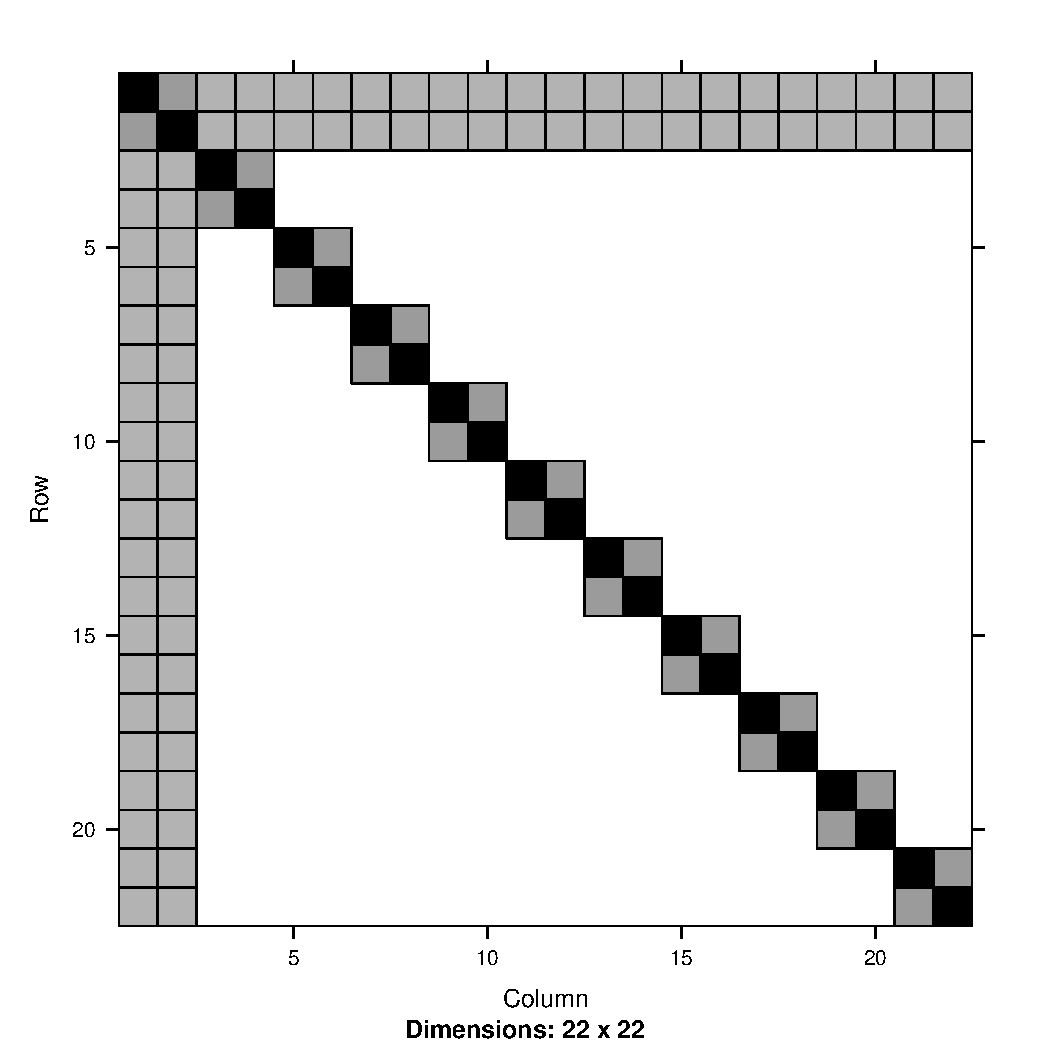
\includegraphics[width=0.95 \textwidth]{mX_mZ_mLambda.pdf}
		\caption{Covariance matrix -- Fixed effects before random effects}
		\label{fig:covfixedrandom}
	\end{figure}
		
	\begin{figure}[p]
		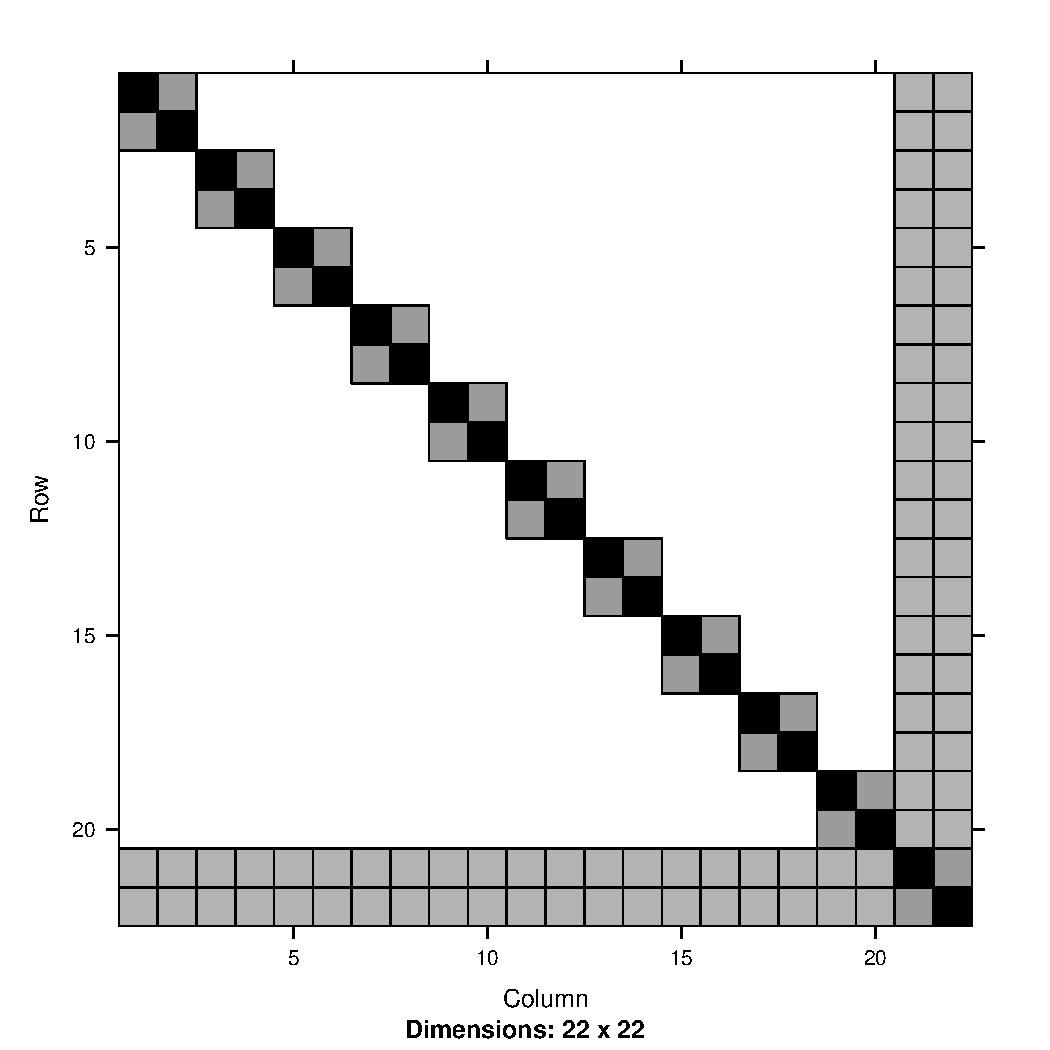
\includegraphics[width=0.95 \textwidth]{mZ_mX_mLambda.pdf}
		\caption{Covariance matrix -- Random effects before fixed effects}
		\label{fig:covrandomfixed}
	\end{figure}
							      				      			      			      			      	
	\begin{figure}[p]
		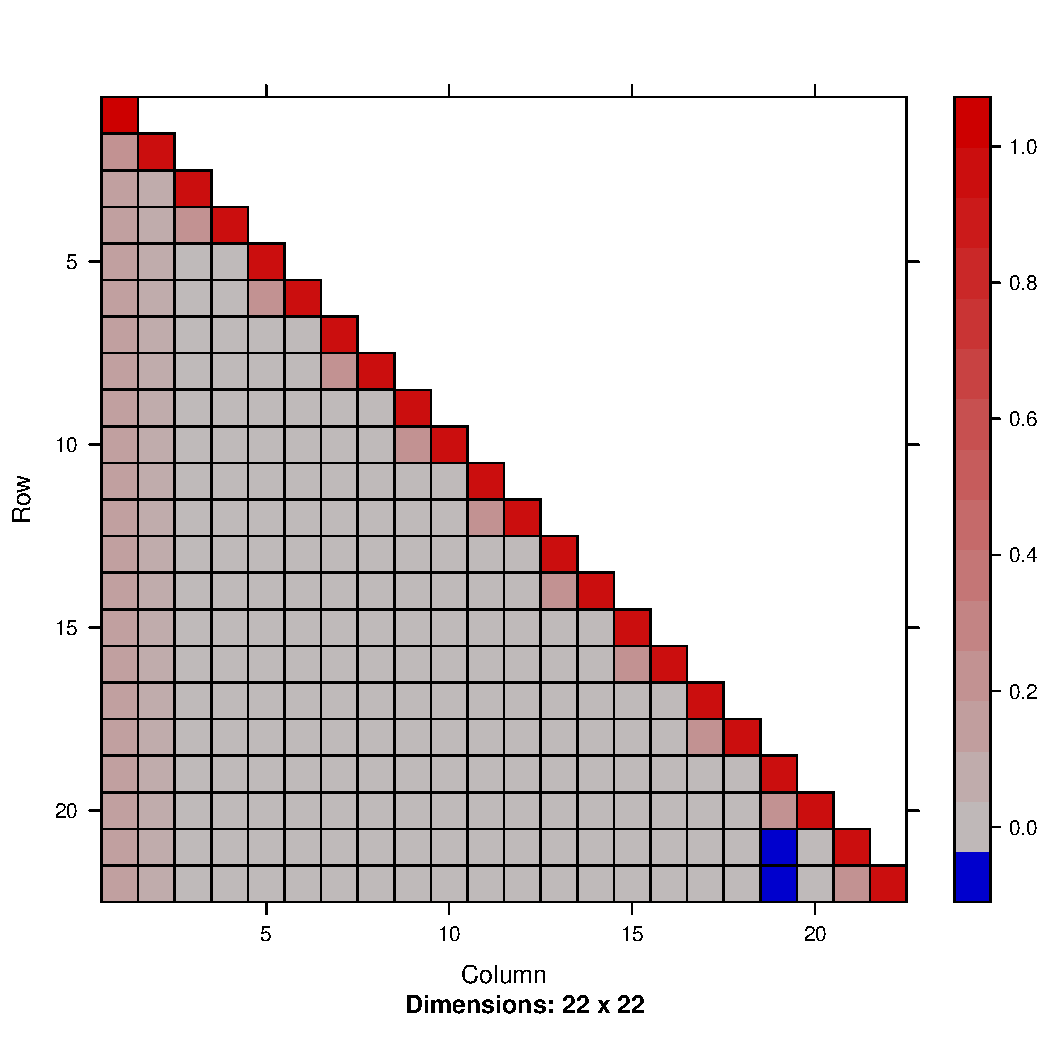
\includegraphics[width=0.95 \textwidth]{mX_mZ_cholesky.pdf}
		\caption{Cholesky factor -- Fixed effects before random effects}
		\label{fig:cholfixedrandom}
	\end{figure}
		
	\begin{figure}[p]
		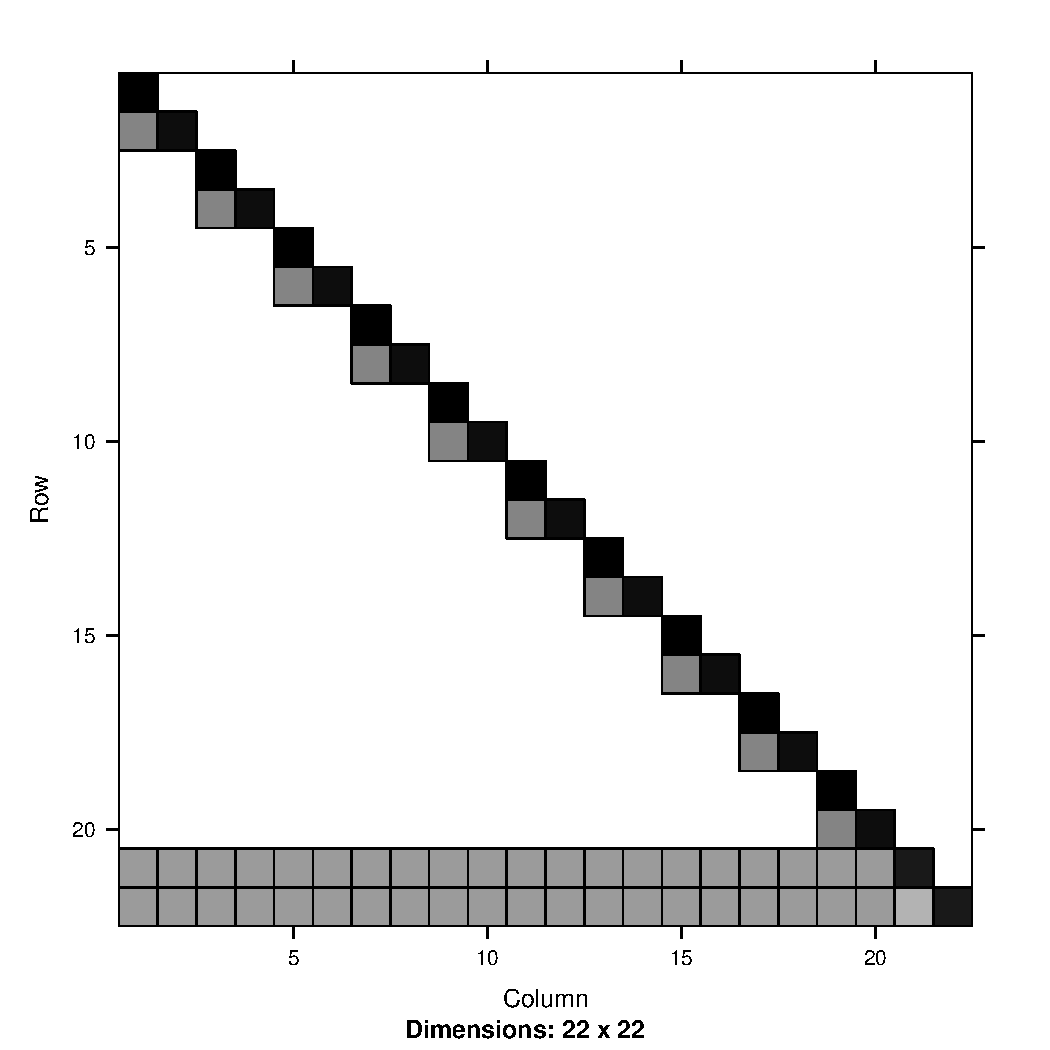
\includegraphics[width=0.95 \textwidth]{mZ_mX_cholesky.pdf}
		\caption{Cholesky factor -- Random effects before fixed effects}
		\label{fig:cholrandomfixed}
	\end{figure}
		
	\subsubsection{Precision parameterisation $\mLambda = (\mR^\top \mR)^{-1}$}
			
	\noindent The second variant of the Gaussian Variational Approximation algorithm is similiar to the first, but
	instead of optimising the Gaussian variational lower bound with respect to $\vmu$ and the Cholesky factor
	$\mR$ of $\mLambda$, we instead optimise the Cholesky factor of the inverse of $\mLambda$ i.e. $\mLambda =
	(\mR \mR^\top)^{-1}$.
	
	The Gaussian variational lower bound in this parameterisation is
	\begin{align*}
		\log \underline{p}(\vmu, \mLambda; \vy) & = \quad \vy\mP\mC \vmu - \vp^\top \exp\{\mC \vmu + \tfrac{1}{2} \text{diag}(\mC \mLambda \mC^\top)\} - \tfrac{1}{2} \vmu^\top \mSigma^{-1} \vmu - \tfrac{1}{2} \tr{(\mSigma^{-1} \mLambda)} \\
		                                        & \quad- \tfrac{p}{2} \log{(2 \pi)} + \tfrac{1}{2} \log{|\mSigma^{-1}|} + \tfrac{p}{2} \log{(2 \pi)} + \tfrac{p}{2} - \log{|\mR|}                                             
	\end{align*}
			
	\noindent The derivative with respect to $\vmu$ is the same as that in the first variant of the algorithm, but 
	as the parameterisation of $\mLambda$ has changed, the  derivative with respect to $\mLambda$ becomes
	\begin{align*}
		\frac{\partial \log \underline{p}(\vmu, \mLambda; \vy)}{\partial \mLambda}
		  & = \hphantom{-}(\mLambda^{-1} + \mH)(-\mLambda \mR \mLambda) \\
		  & = -(\mI + \mH\mLambda)\mR\mLambda                           \\
		  & = - (\mR\mLambda + \mH\mLambda\mR\mLambda)                  
	\end{align*} 
			
	\noindent where $\mH = (\mP \mC)^\top \text{diag}(\exp(\mC \vmu + \frac{1}{2} \mC \mLambda \mC^\top)) \mP \mC - \mSigma^{-1}$.
			
	\subsubsection{GVA fixed point} 	% Fixed point update of \mLambda
	This variant of the algorithm uses Newton-Raphson-like fixed point updates on the Gaussian variational lower
	bound. We optimise the same variational lower bound as in the covariance parameterisation above, using the
	derivatives below. The steps are presented in Algorithm \ref{alg:algorithm_nr} where	
	\begin{align*}
		\frac{\partial \log \underline{p}(\vmu, \mLambda; \vy)}{\partial \vmu}     & = \quad \mC^\top\vp \left \{\vy - \mC\exp(\mC \vmu + \tfrac{1}{2} \text{diag}(\mC \mLambda \mC^\top)) \right \} - \mSigma^{-1} \vmu \text{ and} \\
		\frac{\partial \log \underline{p}(\vmu, \mLambda; \vy)}{\partial \mLambda} & = -\mC^\top \text{diag}(\vp^\top \exp(\mC \vmu +\tfrac{1}{2} \text{diag}(\mC \mLambda \mC^\top))) - \mSigma^{-1}.                             
	\end{align*}
	As this algorithm involves a simple Newton-Raphson style update step, it is computationally simple to
	implement, but potentially unstable as there is no adaptation of step size, as in L-BFGS-B.

	For efficiency, the inversion of $\mLambda$ within the algorithm was implemented using the block inverse 
	formula, where	the matrix was partitioned
	\[
		\mLambda =
		\begin{pmatrix}
			\mLambda_{\vbeta \vbeta} & \mLambda_{\vbeta \vu} \\
			\mLambda_{\vbeta \vu}^\top & \mLambda_{\vu \vu}
		\end{pmatrix}
	\]
	where $\mLambda_{\vbeta \vbeta}$ is the $p \times p$ approximation of the fixed effects covariance, $\mLambda_{\vbeta \vu}$ is the $p \times mb$
	approximation of the covariances between the fixed and random effects and $\mLambda_{\vu \vu}$ is the $mb \times mb$
	approximation of the random effects covariance.

	Sometimes in the course of  executing the algorithm, we observed numerical issues which had to be dealt
	with in order for the algorithm to successfully complete. If the block $\mLambda_{\vu \vu}$ cannot be inverted on an
	iteration, we reverted to $\vmu$ and $\mLambda$ from the previous iteration. If after updating $\vmu$
	any element is NaN, we reverted to the $\vmu$ and $\mLambda$ from the previous iteration. This greatly
	improved the stability of the algorithm.
	
	\begin{algorithm}
		\caption[Algorithm GVA NR]{Iterative scheme for obtaining optimal $\vmu$ and $\mLambda$
			given $\vy$, $\mC$ and $\vp$}
		\label{alg:algorithm_nr}
		\begin{algorithmic}
			\REQUIRE $\frac{\partial \log \underline{p}(\vmu, \mLambda; \vy)}{\partial \vmu} = \mP \mC (\vy - \mC^\top \exp(\mC \vmu + \frac{1}{2} \text{diag}{(\mC \mLambda \mC^\top)})) - \mSigma^{-1} \vmu$.
			% Fit \vmu, \mLambda using Laplace approximation
			\WHILE{the increase in $\log{\underline{p}}(\vmu, \mLambda; \vy)$ is significant}
			% \vmu, \mLambda
			\STATE $\mLambda^{-1} = \left \{ \mP^\top \mC^\top \exp(\mC \vmu + \frac{1}{2} \text{diag}(\mC \mLambda \mC^\top)) \mC \mP \right \}$ \\ [1ex]
			Calculate \STATE $\mLambda \leftarrow \left (\mLambda^{-1} \right )^{-1}$  using the block inverse formula \\ [1ex]
			If $\mLambda_{\vu \vu}$ cannot be inverted in the above calculation, revert to $\vmu$ and $\mLambda$ from the previous iteration \\ [1ex]
			\STATE $\frac{\partial \log \underline{p}(\vmu, \mLambda; \vy)}{\partial \vmu} = -\mC^\top \text{diag}[\vp^\top \exp\{\mC \vmu + \frac{1}{2} \text{diag}(\mC \mLambda \mC^\top)\}] - \mSigma^{-1}$ \\ [1ex]
			\STATE $\vmu \leftarrow \vmu + \mLambda \left \{ \frac{\partial \log \underline{p}(\vmu, \mLambda; \vy)}{\partial \vmu} \right \}$ \\ [1ex]
			If any element of $\vmu$ is NaN, revert to $\vmu$ and $\mLambda$ from the previous iteration
			\ENDWHILE
		\end{algorithmic}
	\end{algorithm}
			
	% Splines
			
	\section{Parameterisations and computational cost of Gaussian Variational Approximation approaches}
	\label{sec:param}
	\subsection{Covariance parameterisation of $\mLambda$}
	
	To ensure symmetry of $\mLambda$, we parameterise the optimisation problem in terms of $\mLambda$'s
	Cholesky factor  $\mLambda = \mR^\top \mR$. We optimise over the space $(\vmu, \overline{\mR})$, where $\vmu
	\in \R^{p + m}b$ and $\overline{\mR}$ is a lower-triangular $(p + mb) \times (p + mb)$ matrix. Then
			
	\begin{equation*}
		\mR_{ij} =
		\begin{cases}
			\exp(\overline{\mR}_{ij}), & i = j             \\
			\overline{\mR}_{ij},       & i > j             \\
			0,                         & \text{otherwise}, 
		\end{cases}
	\end{equation*}
			
	\noindent exponentiating the diagonal to ensure positive-definiteness of $\mR$. We parameterise $\mLambda$
	as $\mLambda = \mR \mR^\top$ so that is is guaranteed to be symmetric, and we only have $p(p-1)/2$ 
	parameters to deal with instead of $p^2$ parameters, some of which are constrained. 
	
	This parameterisation can lead to numeric overflow when the diagonals of $\overline{\mR}$ become moderately
	large, which can lead to singular matrices when attempting to invert $\mLambda$. We dealt with this by
	defining a piecewise function which is exponential for arguments less than $t$, and quadratic for arguments
	greater than or equal to $t$
	$$
	f(r_{ij}) =
	\begin{cases}
		e^{r_{ij}}, r_{ij} < t                   \\
		a r_{ij}^2 + b r_{ij} + c, r_{ij} \geq t 
	\end{cases}
	$$
	and then choosing the co-efficients $a$, $b$ and $c$ such that the function, first and second derivatives would
	agree at $r_{ij} = t$.
	
	To find the co-efficients $a$, $b$ and $c$, we solved the system of equations formed by repeatedly 
	differentiating the quadratic at $r_{ij} =  t$ and equating it with $e^t$
	$$
	\begin{array}{lllll}
		e^t & = & a t^2 & + \quad b t & + \quad c \\
		e^t & = &       & \quad 2a t  & + \quad b \\
		e^t & = &       &             & \quad 2a  \\
	\end{array}
	$$
	to obtain $a = e^t / 2$, $b = (1 - t) e^t$ and $c = \{1 - t^2/2 - (1 - t) t\} e^t$.
	
	We also addressed the overflow problem by working with the Cholesky factorisation of $\mLambda^{-1}$
	rather than $\mLambda$, allowing us to solve a system of equations rather than invert and multiply by a
	matrix, which is also faster and more numerically stable. We use knowledge of the regression  model we are
	fitting to specify a sparse matrix structure, greatly reducing the dimension of   the problem and thus
	improving both computational speed and numeric accuracy.
	
	% \noindent By noticing that the lower rows of the product depend on the higher rows of the Cholesky factor, we
	% observe that by re-ordering the fixed and random effects in $\mLambda$ so that the , we arrive at a covariance structure which is sparse in the first diagonal block. Thus the Cholesky factor of $\mLambda$ that we optimise over is as sparse as possible. This reduces the dimension of the optimisation problem we have to solve from
	% $\BigO(np^2)$ to $\BigO(np)$.
		
	Any symmetric matrix $\mLambda$ can be written as a product of its' Cholesky factors, $\mLambda =
	\mR \mR^\top$ where $\mR$ is lower triangular. $\mR$ is unique if $\mR_{ii} \geq 0$.
		
	\begin{align*}
		&\begin{pmatrix}
		\mR_{11}          & 0                                    & 0                                     \\
		\mR_{21}          & \mR_{22}                             & 0                                     \\
		\mR_{31}          & \mR_{32}                             & \mR_{33}                              
		\end{pmatrix}
		\begin{pmatrix}
		\mR_{11}          & \mR_{21}                             & \mR_{31}                              \\
		0                 & \mR_{22}                             & \mR_{32}                              \\
		0                 & 0                                    & \mR_{33}                              
		\end{pmatrix}
		\\
		=& \begin{pmatrix}
		\mR_{11}^2        &                                      & \text{symmetric}                      \\
		\mR_{21}\mR_{11} & \mR_{21}^2 + \mR_{22}^2 \\
		\mR_{31} \mR_{11} & \mR_{31}\mR_{21} + \mR_{32} \mR_{22} & \mR_{31}^2 + \mR_{32} ^2 + \mR_{33}^2 
		\end{pmatrix}.
	\end{align*}
	
	\noindent We exploit this structure. By interchanging the fixed and random effects in the design matrix $\mC = [\mX \mZ]$ to $\mC = [\mZ \mX]$, and re-ordering the dimensions of $\vmu, \mLambda$ and $\mSigma$ in the same manner, the independence between the
	blocks relating to the random effects in $\mZ$ induce sparsity in the Cholesky factor $\mR$ of
	$\mLambda^{-1}$, as can be seen in Figures \ref{fig:covfixedrandom}, \ref{fig:covrandomfixed},
	\ref{fig:cholfixedrandom} and \ref{fig:cholrandomfixed}. Thus the Gaussian $q(\vnu) \sim \N(\vmu, \mLambda)$ can be optimised over a space of dimension $\frac{1}{2} p (p + 1) + pq + \frac{1}{2} q (q + 1)$ rather than dimension
	$\frac{1}{2} (p + mq) (p + mq + 1)$ as in the dense parameterisation. This leads to subtantial performance gains
	when $m$ is large, as is typically the case in problems of practical importance such as longitudinal or 
	clinical trials with many subjects or the application presented in Section \ref{sec:application}.
			
	By re-ordering the fixed and random effects in $\mLambda$, we end up with a covariance structure which is 
	sparse in the first diagonal block.
	
	\subsection{Precision parameterisation}
	
	We optimise over the space $(\vmu, \overline{\mR})$ as before, but now 
			
	\begin{equation*}
		\mR_{ij} =
		\begin{cases}
			\exp(-\overline{\mR}_{ij}), & i = j             \\
			\overline{\mR}_{ij},        & i > j             \\
			0,                          & \text{otherwise}, 
		\end{cases}
	\end{equation*}
		
	\noindent This new choice of parameterisation allows us to calculate $\frac{1}{2} \text{diag}(\mC \mLambda
	\mC^\top)$ by solving the linear systems $\mR \va = \mC_{i}, i=1, \ldots, n$ for   $\va$ and then calculating
	$\va^\top\va$ where $\mC_{i} = $ the $i$th row of $\mC$, rather than calculating $\text{diag}(\mC \mLambda
	\mC^\top)$ directly.
		
	% TODO: We fixed this using safe-exp
	The implementation of these algorithms was not without its' challenges, chiefly numerical issues encountered during testing and verification of the accuracy of the model fitting. Using the exponential function to parameterise the main diagonal coupled with L-BFGS-B's unconstrained line search and \texttt{optim()}'s lack of robustness to infinities lead to many overflow problems which may have been lessened or dealt with entirely by using a function with a less aggressive growth rate, such as an appropriate piecewise quadratic.
		
	The main computational cost is the evaluation of the variational lower bound and its' derivatives. By
	virtue of their dimension, the expressions involving $\mLambda$ dominate the computational cost. The key
	term is $\frac{1}{2} \diag(\mC \mLambda \mC^\top)$. This can be naively calculate by ignoring the
	symmetry in the expression and simply calculating the product $\mC \mLambda \mC^\top$, taking $2 n
	\times (p + m b)^2$ floating point operations, and retaining the diagonal entries of the result. This is
	obviously wasteful, as the off--diagonal entries of the resulting product that has just been computed
	are immediately discarded.
		
	By parameterising $\mLambda$ in terms of its' Cholesky factors and realising that
		
	\[
		\mC \mLambda \mC^\top = \mC \mR \mR^\top \mC^\top
	\]
		
	\noindent and that
		
	\[
		\diag(\mC \mLambda \mC^\top)_{ii} = \mC_{i .} \mR \mR^\top \mC_{i .}^\top, 1 \leq i \leq n
	\]
		
	\noindent we can calculate the products $\mC_{i .} \mR, 1 \leq i \leq n$, using $n \times \frac{1}{2}(p + m
	b)(p + m b   + 1)$ floating point operations, and storing the results of the $i$th product in the $i$th
	element of the   vector $\va$ and then calculate $\diag(\mC \mLambda \mC^\top) = \va^\top \va$.
		
	Moreover, mixed models typically have sparse design matrices, allowing us to encode $\mR$ as a sparse matrix, and	further reduce   this depending on the model. For example, in the random intercept case, only the diagonals of the random effects block need to be non-zero, and hence the above expression can be calculated in
	$\BigO(n)$ floating point operations.
		
	% $\log |\mR|$ can be calculated using only $p + m b$ floating point operations, as $\mR$ is lower triangular.
		
	For the precision parameterisation, we observe that in this parameterisation
	\[
		\diag(\mC \mLambda \mC^\top)_{ii} = \mC_{i .} \mR^{-\top} \mR^{-1} \mC_{i .}^\top, 1 \leq i \leq n,
	\]
		
	\noindent and so by solving $\mR \va = \mC_{i .}^\top$ for $\va$ for all $i$ at a cost of $n \times
	\frac{1}{2} (p + m b) (p + m b + 1)$ floating point operations, and then calculating
	\[
		\diag(\mC \mLambda \mC^\top)_{ii} = \va^\top \va, 1 \leq i \leq n,
	\]
		
	\noindent we can then calculate $\diag(\mC \mLambda \mC^\top)$.
		
	As above, by using our knowledge of the model being fit we can encode $\mR$ sparsely to decrease
	the required   computation still further. In the random intercept model case, the computational cost will drop
	to   $n \times [m + \frac{1}{2} p (p + 1) + p \times m b]$.
				
			\section{Numerical results}
			\label{sec:results}
					
			The accuracy of each model fitting algorithms presented in Section \ref{sec:gaussian} was assessed by
			comparing the approximating distribution of each parameter with the posterior distribution of Monte Carlo
			Markov Chain samples of that parameter. 1 million Monte Carlo Markov Chain samples were generated using Stan.
			The accuracy of examples of random intercept, random slope and spline models were evaluated using this method.
					
			\subsection{Simulated data}
					
			For each of these simulations, the model is as presented in Section \ref{sec:model}.
					
			Several common application scenarios were simulated and their accuracy evaluated. A random intercept model was simulated with $\vbeta = (2, 1)^\top$, $\rho = 0.5$, $m = 20$, $n_i = 10$ and $b = 1$. The results are
			presented in Table \ref{tab:accuracy_int}. A random slope model was simulated with $\vbeta = (2, 1)^\top$,
			$\rho = 0.5$, $m = 20$, $n_i = 10$ and $b = 2$. The results are presented in Table \ref{tab:accuracy_slope}.
			Spline model was fit to a data set generated from the function $3 + 3 \sin{(\pi x)}$ on the interval $[-1,
			1]$. The resulting model fits are presented in Figure \ref{fig:spline}.
					
			To assess the speed of each approach, a test case was constructed of a random slope model with $m=50$ groups,	each containing $n_i = 100$ individuals. A model was then fit to this data set ten times using each algorithm, and the results averaged. They are presented in Table \ref{tab:application_slope_speed}.

			\begin{table}
				\caption{Table of results - Speed}
				\label{tab:application_slope_speed}
				\begin{tabular}{|l|rr|}
					\hline
					Algorithm & Mean (seconds) & Standard deviation (seconds) \\
					\hline
					Laplace's method & 0.37 & 0.07 \\
					GVA covariance parameterisation & 2.04 & 1.24 \\
					% Why is this slower?
					GVA inverse parameterisation & 0.38 & 0.66 \\
					GVA fixed point & 0.05 & 0.07 \\
					\hline
				\end{tabular}
			\end{table}

			% The stability of the algorithms was confirmed by running them on 10,000 different data sets that were randomly
			% generated after having initialised the random number generator with different seeds.
					
			Median accuracy of the algorithms was assessed by running them on 100 randomly generated data sets. The	results are presented in Figure \ref{fig:median_accuracy_intercept} and Figure
			\ref{fig:median_accuracy_slope}.
					
			% Figure: Median accuracy graph intercept
			\begin{figure}
				\begin{center}
					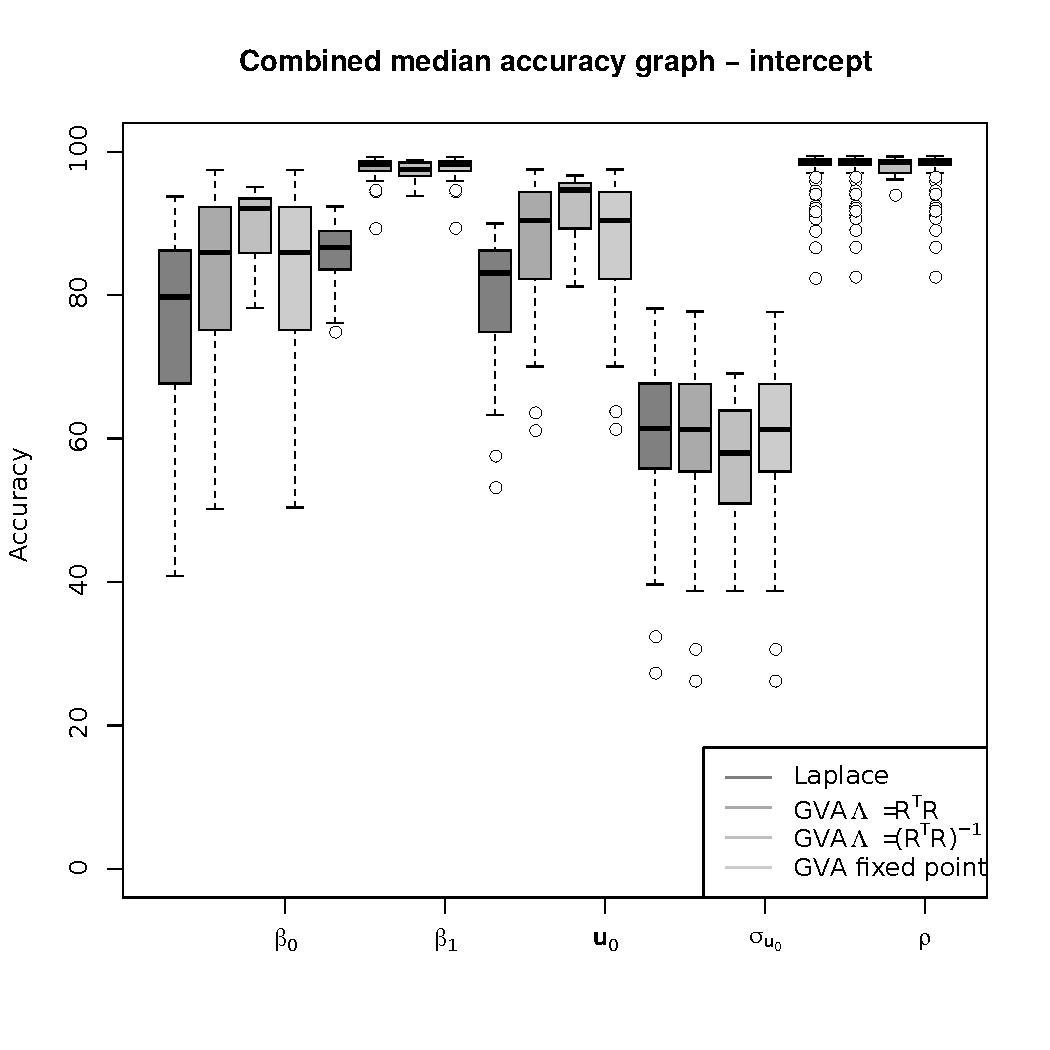
\includegraphics[width=0.95\textwidth, height=100mm]{code/results/median_accuracy_combined_intercept.pdf}
					\caption{Median accuracy of random intercept}
					\label{fig:median_accuracy_intercept}
				\end{center}
			\end{figure}
					
			% Figure: Median accuracy graph slope
			\begin{figure}
				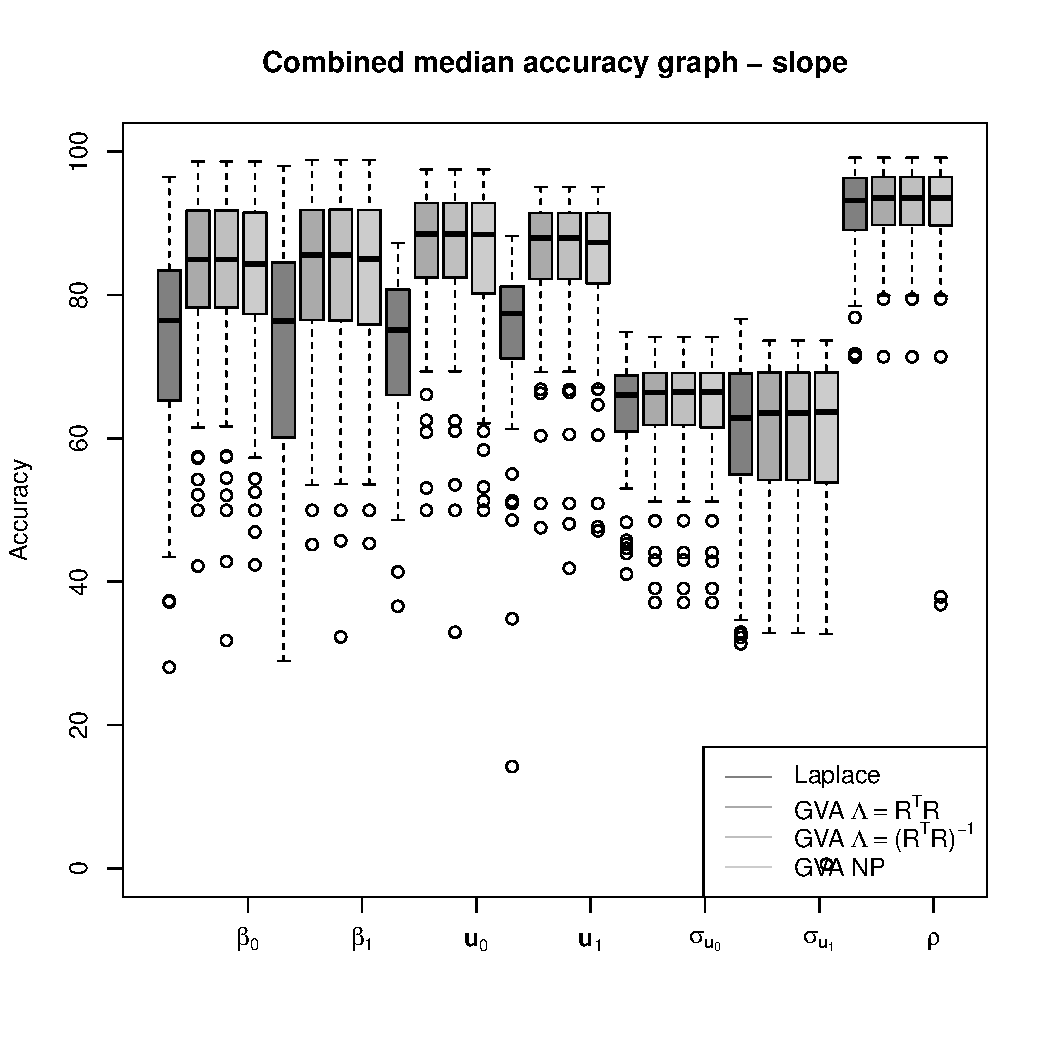
\includegraphics[width=0.95\textwidth, height=120mm]{code/results/median_accuracy_combined_slope.pdf}
				\caption{Median accuracy of slope}
				\label{fig:median_accuracy_slope}
			\end{figure}
					
			% Table of accuracy results - intercept model
			\begin{table}
				\caption{Table of accuracy - Random intercept model}
				\label{tab:accuracy_int}
				\begin{tabular}{|l|rrrr|}
					\hline
					                   & Laplace's Method & GVA $(\mLambda = \mR \mR^\top)$ & GVA NP $(\mLambda = (\mR \mR^\top)^{-1})$ & GVA FP \\
					\hline
					$\vbeta_1$         & $85\%$           & $90\%$                          & $91\%$                                    & $90\%$ \\ 
					$\vbeta_2$         & $76\%$           & $98\%$                          & $99\%$                                    & $99\%$ \\ 
					Mean of $\vu$      & $81\%$           & $94\%$                          & $94\%$                                    & $94\%$ \\
					$\sigma^2_{\vu_1}$ & $66\%$           & $66\%$                          & $66\%$                                    & $66\%$ \\ 
					$\rho$             & $99\%$           & $99\%$                          & $99\%$                                    & $99\%$ \\ 
					\hline
				\end{tabular}
			\end{table}
					
			\begin{table}
				\caption{Table of accuracy - Random slope model}
				\label{tab:accuracy_slope}
				\begin{tabular}{|l|rrrr|}
					\hline
					                   & Laplace's Method & GVA $(\mLambda = \mR \mR^\top)$ & GVA $(\mLambda = (\mR \mR^\top)^{-1})$ & GVA FP \\
					\hline
					$\vbeta_1$         & 67\%             & 88\%                            & 88\%                                   & 88\%   \\
					$\vbeta_2$         & 70\%             & 89\%                            & 88\%                                   & 89\%   \\
					Mean of $\vu$      & 70\%             & 91\%                            & 91\%                                   & 91\%   \\
					$\sigma^2_{\vu_1}$ & 71\%             & 73\%                            & 73\%                                   & 73\%   \\
					$\sigma^2_{\vu_2}$ & 68\%             & 69\%                            & 69\%                                   & 69\%   \\
					$\rho$             & 91\%             & 90\%                            & 90\%                                   & 90\%   \\
					\hline
				\end{tabular}
			\end{table}
					
			% \begin{table}
			% \caption{Table of accuracy - Splines}
			% \label{tab:accuracy_spline}
			% \begin{tabular}{|l|l|}
			% \hline
			% Approximation & Accuracy \\
			% \hline
			% Laplace's Method & 0.969 \\
			% GVA & 0.969 \\
			% GVA NP & 0.969 \\
			% GVA NR & 0.969 \\
			% \hline
			% \end{tabular}
			% \end{table}
					
			\begin{figure}
				\label{fig:spline}
				\caption{Comparison of VB and MCMC spline fits with the true function}
				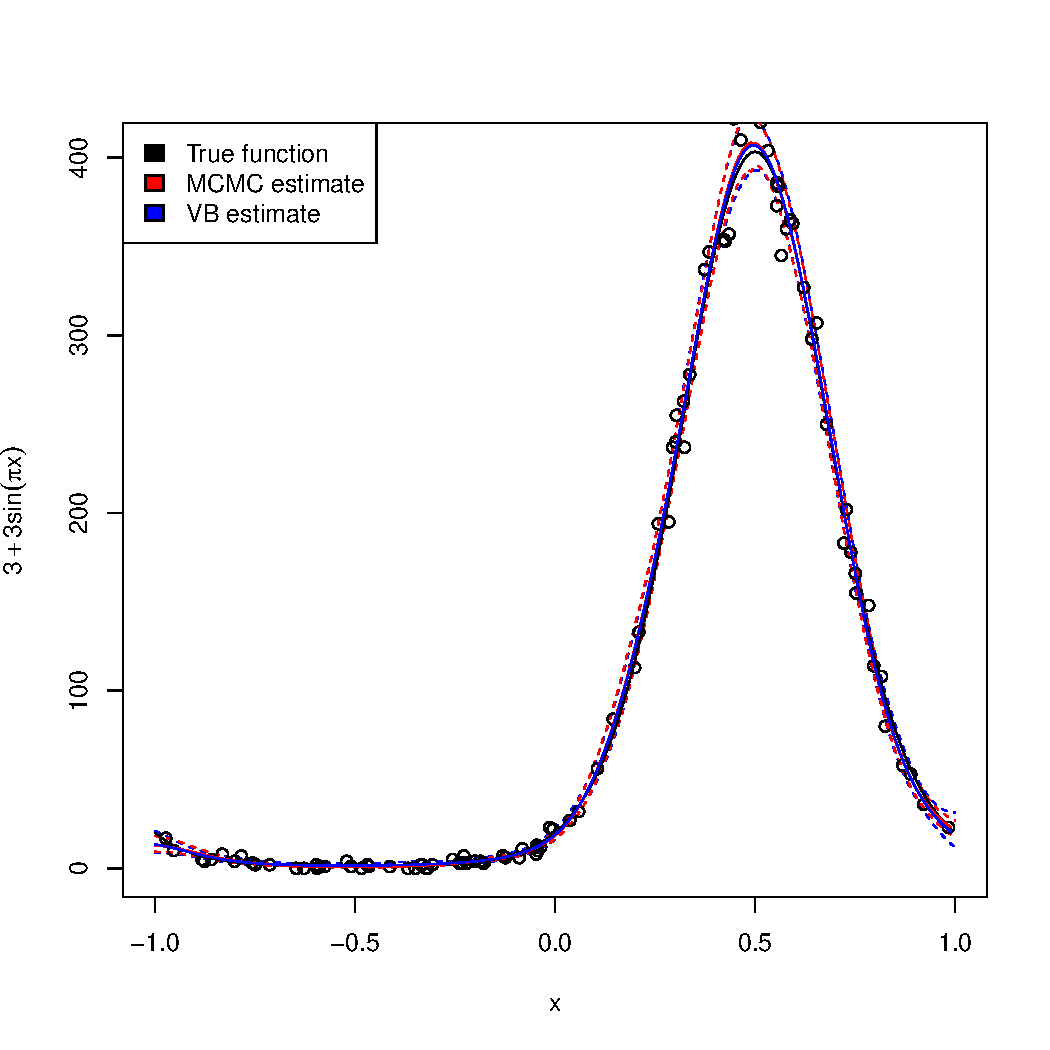
\includegraphics[width=0.95 \textwidth, height=100mm]{code/results/accuracy_plots_spline_gva2.pdf}
			\end{figure}
					
			% Graphs - exactly what sort of graphs do we need?
			% Median accuracy
			% Increase in lower bound
			% MCMC posterior, with approximating posterior for at least one or two of the
			% key parameters, such as, say, vbeta[2]
					
			\subsection{Numerical stability of the parameterisation}
			
			In the process of performing numerical experiments, we discovered that our model fitting software was 
			prone to numeric overflow due to the log link in our model and the exponentiation of the diagonals of the
			Cholesky factors in the covariance parameterisation of the Gaussian Variational Approximation of $\vnu$.
			
			We dealt with this difficulty by developing a 'safe exponential' parameterisation for the diagonals of the
			Cholesky factors. The parameterisation is exponential up to a threshold $t$, and then quadratic beyond that
			threshold.
			
			The stability of this scheme was tested by calculating the accuracy of the approximations fit with a range
			of safe exponential thresholds, the results of which are presented in Figure \ref{fig:stability_accuracy}.
			The variational approximation was found to be stable, with the accuracy largely insensitive to the choice of
			threshold.
			
			\begin{figure}
				\includegraphics[width=0.95 \textwidth]{code/stability_intercept.pdf}
				\label{fig:stability_accuracy}
				\caption{Accuracy of approximation of parameters versus the safe exponential threshold}
			\end{figure}
			
			We repeated our numerical experiments with the new parameterisation, varying the threshold within reasonable
			bounds and found that the numerical experiments no longer resulted in overflow, and that the numerical accuracy
			of the approximation was still very good.
			
			The stability of the GVA algorithm with the parameterisation $\mLambda = (\mR^\top \mR)^{-1}$ depends on the
			threshold chosen for the safe exponential function. When the threshold is set to $2$, the algorithm is stable
			for all starting points within the grid except $6$. When the threshold is set to $\infty$, equivalent to using
			the naive $\exp$ parameterisation, the algorithm encounters numerical errors for every starting point on the 
			grid.
				
			\subsection{Stability of the GVA precision parameterisation algorithm for different starting points}
					
			The numerical stability of each fitting algorithm in Section \ref{sec:gaussian} was assessed by initialising
			each algorithm from a range of different starting points. Errors due to numerical instability and the fitted
			$\vmu$ were recorded for each starting point.
					
			A data set of 100 individuals in ten groups ($m=10$) was generated from a model with a fixed intercept and
			slope, and a random intercept. $\vmu$ was initialised from a grid of points on the interval $[-4.5, 5]$ for
			intercept and slope, spaced $0.1$ apart. The error counts are presented in Table
			\ref{tab:stability_results}. Plots of the starting locations which resulted in numerical errors when the
			fitting algorithm was run are presented in \ref{fig:stability_locations_gva}.
					
			\begin{table}
				\begin{tabular}{|l|r|}
					\hline
					Algorithm                            & Error count \\
					\hline
					Laplace's algorithm                  & 12          \\
					GVA $\mLambda = \mR^\top \mR$        & 1,306       \\
					GVA $\mLambda = (\mR^\top \mR)^{-1}$ & 6           \\
					GVA NR fixed point                   & 992         \\
					\hline
				\end{tabular}
				\caption{Count of numerical errors for each algorithm during stability tests}
				\label{tab:stability_results}
			\end{table}

			The GVA algorithm with the $\mLambda = (\mR \mR^\top)^{-1}$ parameterisation was less prone to
			instability due to starting point when the safe exponential parameterisation was used then when it was
			not used, as can be seen from Figure \ref{fig:stability_locations_gva}. % FIXME: Add error counts
					
			\begin{figure}
				\includegraphics[width=0.95 \textwidth]{code/safe_exp_stability.pdf}
				\includegraphics[width=0.95 \textwidth]{code/no_safe_exp_stability.pdf}
				\label{fig:stability_locations_gva}
				\caption{Starting locations which caused the GVA fitting algorithm to fail with numeric errors. The true model had fixed parameters $\vbeta = (2, 1)^\top$ and random intercepts. There were ten groups in the
					hierarchical model each	with ten individuals $(m=10, n_i=10)$}
			\end{figure}

			\subsection{Stability of the GVA fixed point algorithm for different starting points}

			The naive fixed point algorithm was extremely unstable for many starting points, as can be seen from
			Figure \ref{fig:stability_locations_nr}. The variant of the algorithm which checked whether the
			inversion of the $\mLambda_{\vu \vu}$ block of $\mLambda$ was performed successfully was much more
			stable, and did not suffer from any numeric errors at all over the range of starting points we tested.
			The algorithm is able to abort safely, and allow the Variational Bayes algorithm to update the other
			parameters before trying to fit the Gaussian component of the model again until the correct parameters
			are accurately estimated.

			\begin{figure}
				\includegraphics[width=0.95 \textwidth]{code/local_solutions_gva_nr_error_locations_no_protections.pdf}
				\label{fig:stability_locations_nr}
				\caption{Starting locations which caused the NR fitting algorithm to fail with numeric errors. The true model 						had fixed parameters $\vbeta = (2, 1)^\top$ and random intercepts. There were ten groups in the
					hierarchical model each	with ten individuals $(m=10, n_i=10)$}
			\end{figure}
			
			\section{Application}
			\label{sec:application}
			
			\subsection{Poisson example without zero-inflated component -- Police stops}
			The data set used for this example was the police stop example from Chapter 15 of \citep{Gelman2007}.
			The model fit was
			\begin{align*}
				\vy_{ep}        & \sim \text{Poisson}(n_{ep} e^{\beta_0 + \beta_e \text{ethnicity}_e + \alpha_{c} \text{crime} + \vu_p}), \\
				\valpha				& \sim \N(0, \sigma_\valpha^2),	\\
				\vbeta        & \sim \N(0, \sigma_\vbeta^2), \text{ and }\\
				\vu_p         & \sim \N(0, \sigma_\vu^2)
			\end{align*}
			where $p$ is the $p$-th precinct, and $e$ is the $e$-th ethnicity (blacks, hispanics or whites), and $c$ is
			the $c$-th category of crime (violent crimes, weapons crimes, propery crimes, drug crimes). The random 
			intercepts $u_p$ allow for variation in the base rates of stops across precincts,
			the co-efficients $\beta_j$ measure the effect of ethnicity on the rate of police stops and
			the co-efficients $\alpha_k$ measure the effect of each type of crime on the rate.
			The model finds the relationship between the number of police stops in each precinct and 
			ethnicity	for each type of crime.
			
			The model was fit using the GVA algorithm with the $\mLambda = (\mR^\top \mR)^{-1}$ parameterisation, using
			the prior $a_\rho = 3$, $b_\rho = 1$ on $\rho$. Accuracy of the approximation was assessed by comparing the
			fitted distribution for each parameter to a kernel density estimate of the parameter's distribution from
			1 million samples from the equivalent model fitted using Stan. The results are presented in Table
			\ref{tab:application_police_stops}. Figure \ref{fig:police_stops}
			
			\begin{figure}
			\includegraphics[width=0.95 \textwidth]{code/results/accuracy_plots_application2_GVA_inv_par-highlights-nup.pdf}
			\caption{Accuracy of parameter estimates for police stops}
			\label{fig:police_stops}
			\end{figure}

			% Table of results
			\begin{table}
				\caption{Table of results - Police stops}
				\label{tab:application_police_stops}
				\begin{tabular}{|l|rrrr|}
					\hline
					Covariate                     & Posterior Mean & Lower 95\% CI & Upper 95\% CI & Accuracy \\
					\hline
					Intercept [African-Americans] & 4.04          & 3.98           & 4.07          & 82.4\%   \\
					$\beta_2$ [hispanics]         & -0.45         & -0.46          & -0.43         & 98.1\%   \\
					$\beta_3$ [whites]            & -1.38         & -1.40          & -1.37         & 98.5\%   \\
					$\alpha_1$ [weapons crimes]   & 0.58          & 0.57           & 0.59          & 89.2\%   \\
					$\alpha_2$ [property crimes]  & -0.19         & -0.21          & -0.17         & 92.2\%   \\
					$\alpha_3$ [drug crimes]      & -0.750        & -0.77          & -0.73         & 94.9\%   \\
					Random intercept              & 1.321         & -0.190         & 2.202         & 86.7\%   \\
					$\sigma^2_{\vu}$              & 8.57          & 1.02           & 24.35         & 49\%     \\
					\hline
				\end{tabular}
			\end{table}
			
			% Table of speeds
			\begin{table}
				\begin{tabular}{|ll|}
					\hline
					Algorithm & Time  in seconds \\
					\hline
					Laplace & 0.24 \\
					GVA covariance parameterisation & 6.02 \\
					GVA inverse paramaterisation & 3.92 \\
					GVA fixed point & 0.18 \\
					\hline
				\end{tabular}
				\caption{Table of speeds - Police stops}
				\label{tab:police_stop_speeds}
			\end{table}
			
			% TODO: You need to describe the data set and the model.
			\subsection{Zero--inflated example -- Cockroaches in Apartments data set from Gelman}
			The model described in this section was fit
			 to the cockroach data set from \S 6.7 of \citep{Gelman2007}, taken from a study
			on the effect of integrated pest management in controlling cockroach levels in urban apartments. The data
			set contains data on 160 treatment and 104 control apartments, along with the response $y_i$ in each
			apartment of the number of cockroaches caught in a set of traps. The apartments had the traps deployed for
			different numbers of days, referred to as trap days, which was handled by using a log offset
			\citep{Agresti2002}. The predictors in the data set included the pre-treatment roach level, a treatment
			indicator, the time of the observation and an indicator for whether the apartment is in a senior building
			restricted to the elderly.
					
			In the example application presented in this paper, the zero component represents an apartment completely free of roaches, while the non-zero component represents an apartment where roaches have been able to live and reproduce, possibly in spite of pest control treatment aimed at preventing them from doing so.

			The model fit was
			\begin{align*}
				y_i &= \begin{cases}
				0 \phantom{-} \text{if} \phantom{-} R_i = 0 \\
				\text{Poisson}(e^{\mX_i \vbeta + \mZ_i \vu}) \phantom{-} \text{if} \phantom{-} R_i = 1,
				\end{cases} \\
				R_i &\sim \text{Bernoulli}(\rho), \\
				\rho &\sim \text{Beta}(a, b), \\
				\vbeta &\sim \text{N}(\vzero, \sigma^2_\vbeta \mI), \\
				\vu &\sim \text{N}(\vzero, \mSigma), \text{and} \\
				\mSigma &\sim \text{Inverse-Wishart}(\mPsi, v)
			\end{align*}
			with prior parameters $a = 1$, $b = 1$, $\sigma^2_\vbeta = 10^5$, $\mPsi = 10^{-5} \mI$ and $v = 2$.
			These priors were chosen to be vaguely informative for the variance components and a uniform prior for
			the zero-inflation proportion latent variable $\rho$. The fixed effects covariates included in the
			model were time in days and time in days $\times$ pest control treatment. A random intercept to account
			for variation between the apartment buildings was included.
					
			The GVA algorithm with the $\mLambda = (\mR^\top \mR)^{-1}$ parameterisation was used to fit a random
			intercept model to the Roaches data set provided by Andrew Gelman. The fitted co-efficients and accuracy
			results are presented in Table \ref{tab:application_roaches}.
					
			%       lci  uci
			% 1  3.179 3.157 3.201
			% 2 -0.046 -0.053 -0.039
			% 3 -0.420 -0.434 -0.406
			% 1 -0.976 -1.015 -0.936
			% 2 -0.309 -0.323 -0.295
			% 3 -0.947 -0.963 -0.930
			% 4 -2.129 -2.384 -1.874
			% 5 -3.230 -3.490 -2.970
			% 6 -3.099 -3.404 -2.794
			% 7 -1.290 -1.326 -1.255
			% 8 -0.956 -0.991 -0.921
			% 9 -2.404 -2.600 -2.209
			% 10 -1.076 -1.123 -1.029
			% 11 -1.079 -1.107 -1.052
			% 12 -1.681 -1.737 -1.624
					
			%> round(cbind(fit1$vmu, lci, uci), 3)
			% fit1$a_rho
			% [1] 377.2375
			% > fit1$b_rho
			% [1] 152.7625
					
			\begin{table}
				\begin{tabular}{|l|rrrr|}
					\hline
					Covariate          & Posterior Mean & Lower 95\% CI & Upper 95\% CI & Accuracy \\
					\hline
					Intercept          & 3.42						& 3.2 					& 3.65          & 95\%     \\
					Time               & $-$0.14        & $-$0.05       & $-$0.02       & 96\%     \\
					Time:Treatment     & $-$0.31        & $-$0.43       & $-$0.14       & 96\%     \\
					Random intercept   & $-$1.60        & $-$1.71       & $-$1.49       & 90\%     \\
					$\sigma^2_{\vu_1}$ & 3.29           & 2.02          & 8.48          & 63\%     \\
					$\rho$             & 0.51           & 0.50          & 0.55          & 62\%     \\
					\hline
				\end{tabular}
				\caption{The posterior means, 95\% confidence intervals and accuracy of the fixed and random
									effects, $\sigma_{\vu_1}^2$ and $\rho$ for the Roach model.}
				\label{tab:application_roaches}
			\end{table}

			\begin{table}
				\begin{tabular}{|lr|}
				\hline
				Algorithm & Time in seconds \\
				\hline
				Laplace & 0.49 \\
				GVA & 1.08 \\
				GVA inv. param & 0.81 \\
				GVA fixed point & 0.11 \\
				\hline
				\end{tabular}
				\label{tab:application_roaches_runtime}
				\caption{The runtimes in seconds for fitting algoritms when fitting the roach model.}
			\end{table}
					
			\begin{figure}
				\centering
				% \includepdf[width=75mm,height=75mm,pages={1,2,3,16},nup=2x2]{code/results/accuracy_plots_application_GVA2.pdf}
				\begin{tabular}{@{}c@{\hspace{.5cm}}c@{}}
				\includegraphics[width=0.95 \textwidth]{code/results/accuracy_plots_application_GVA_inv_param-highlights-nup.pdf}
				\end{tabular}
				\caption{Accuracy graphs for roach model}
				\label{fig:accuracy_roach}
			\end{figure}
					
			\subsection{Example - Biochemists}
			The model described in this section was fit to the biochemistry data set analysed by
			\cite{10.2307/2579146}. The sample was taken from 915 biochemistry graduate students. The outcome
			$\vy_i$ is the number of articles published in the last three years of the PhD. The covariates were the
			gender of the student, coded $1$ for female and $0$ for male, the marital status of the student ($1$ for
			married, $0$ for unmarried), the number of children under age six and the prestige of the PhD program.

			In this example application, the zero component represents the number of biochemists who did not publish
			any articles during the last three years of their PhD. Examination of the data reveals that this number
			is higher than would be expected if the data followed a purely Poisson distribution -- 30\% of
			biochemistry graduate students published no articles in their final years whereas a Poisson distribution
			would predict only 18\%. This justifies our choice of model.

			The model fit was
			\[
				y_i = \begin{cases}
				\begin{array}{ll}
				0 &\phantom{-} \text{if} \phantom{-} R_i = 0, \\
				\text{Poisson}(e^{\vbeta_1 + \vbeta_2 \text{female} + \vbeta_3 \text{married} + \vbeta_4 \text{children under age 6} + \vbeta_5 \text{PhD}}) &\phantom{-} \text{if} \phantom{-} R_i = 1,
				\end{array}
				\end{cases}
			\]


			\noindent with priors
			\begin{align*}
			R_i &\sim \text{Bernoulli}(\rho), \\
			\rho &\sim \text{Beta}(A, B), \text { and } \\
			\vbeta &\sim \text{N}(0, \sigma_\vbeta^2 \mI)
			\end{align*}

			\noindent with $A=1$, $B=1$ and $\sigma_\vbeta^2 = 10,000$. The model was fit using the GVA inverse parameterisation algorithm. The resulting model fit is presented in Table \ref{tab:biochemists_results}
			The accuracy of the parameter estimates is presented in Figure
			\ref{fig:biochemists}. As this is a fixed effects model with a large number of samples relative to the
			number of parameters being fit, we are able to estimate all of the parameters with great accuracy.

			\begin{figure}
			\includegraphics[width=0.95 \textwidth]{code/results/accuracy_plots_application_biochemists_GVA_inv_param-nup.pdf}
			\label{fig:biochemists}
			\caption{Accuracy of the approximations of the parameters fit to the biochemists data}
			\end{figure}

			\begin{table}
				\begin{tabular}{|l|rrrr|}
					\hline
					Covariate          & Posterior Mean & Lower 95\% CI & Upper 95\% CI & Accuracy \\
					\hline
					Intercept & 0.86 & 0.65 & 1.06 &  95.17\% \\
					Female & -0.18 & -0.29 & -0.08 &  95.05\% \\
					Married & 0.06 & -0.05 & 0.18 & 95.66\% \\
					Children under age 6 & -0.08 & -0.15 & -0.01 & 96.71\% \\
					PhD & 0.03 & -0.02 & -0.01 & 96.91\% \\
					\hline
				\end{tabular}			
				\label{tab:biochemists_results}
				\caption{The posterior means, 95\% confidence intervals and accuracy of the fixed effects for the 
									Biochemists model.}
			\end{table}

			\begin{table}
				\begin{tabular}{|l|r|}
				\hline
				Algorithm & Time in seconds \\
				\hline
				Laplace & 1.01 \\
				GVA & 0.96 \\
				GVA inv. param & 0.68 \\
				GVA fixed point & 0.41 \\
				\hline
				\end{tabular}
				\label{tab:biochemists_runtime}
				\caption{The runtimes in seconds for fitting algoritms when fitting the Biochemists model.}
			\end{table}
			
			\subsection{Example - Owls}
			The model described in this section was fit to the Owls data set from taken from \cite{zuur_mixed_2009}.
			The sample was 599 observations of owls grouped across 25 nests.The fixed covariates
			fit in the model were food treatment (Deprived or Satiated) and arrival time, a continuous covariate.
			The variation between the 25 different nests sampled from was modelled by a random intercept
			$\vu$.

			The model fit was
			\[
			y_i = R_i e^{\vbeta_2 \text{Food Treatment = Satiated} + \vbeta_3 \text{Arrival Time} + u_n}
			\]
			where $n$ is the $n$-th nest, with priors
			\begin{align*}
			R_i &\sim \text{Bernoulli}(\rho), \\
			\rho &\sim \text{Beta}(A, B), \\
			\vbeta &\sim \text{N}(\vzero, \sigma_\vbeta^2 \mI), \\
			\vu &\sim \text{N}(0, \sigma_\vu^2), \text { and } \\
			\sigma_\vu^2 &\sim \text{Inverse-Gamma}(s, t).
			\end{align*}
			where $\sigma_\vbeta^2=10,000$, $A=1$, $B=1$, $s=10^{-2}$ and $r=10^{-2}$.

			The model was fit using the GVA inverse parameterisation algorithm. The accuracy of the parameter
			estimates is shown in Figure \ref{fig:owls}. The variance component
			The runtime of the algorithms is shown in Table
			\ref{tab:owls_times}. We draw attention to the difference in run-times between the covariance and
			inverse parameterisations -- the inverse parameterisation is 

			\begin{figure}
				\includegraphics[width=0.95 \textwidth]{code/results/accuracy_plots_application_owls_GVA_inv_param-highlights-nup.pdf}
				\caption{Accuracy of the approximations of the parameters fit to the Owls data}
				\label{fig:owls}
			\end{figure}

			\begin{table}
				\begin{tabular}{|l|rrrr|}
					\hline
					Covariate          & Posterior Mean & Lower 95\% CI & Upper 95\% CI & Accuracy \\
					\hline
					Satiated & -0.217 & -0.212 & -0.214 & 97\% \\
					Arrival Time & -0.070 & -0.070 & -0.070 & 73\% \\
					Random intercept (nest) & 0.338 & -5.283 & 5.959 & 84\% \\
					$\sigma_{\vu_1}^2$ & 7.90 & 3.213 & 468.123 & 94\% \\
					$\rho$ & 0.739 & 0.703 & 0.774 & 99\% \\
					\hline
				\end{tabular}			
				\label{tab:owls_results}
				\caption{The posterior means, 95\% confidence intervals and accuracy of the fixed and random
									effects, $\sigma_{\vu_1}^2$ and $\rho$ for the Owls model.}
			\end{table}

			\begin{table}
				\begin{tabular}{|l|r|}
				\hline
				Algorithm & Time in seconds \\
				\hline
				Laplace & 0.71 \\
				GVA covariance parameterisation & 5.66 \\
				GVA inverse parameterisation & 1.88 \\
				GVA fixed point & 0.18 \\
				\hline
				\end{tabular}
				\caption{The runtimes of the fitting algorithms for the Owls model in seconds.}
				\label{tab:owls_times}
			\end{table}

			\section{Discussion}
			\label{sec:discussion}
					
			We have described a Variational Bayes approximation to Zero-Inflated Poisson regression models which allows
			such models to be fit with considerable generality. We have also devised and extensively tested a number of
			alternative approaches for fitting such models, and extended one of these alternative approaches with a new
			parameterisation. Using MCMC methods as the gold standard to test against, we have assessed the accuracy and
			computational speed of these algoritms.
					
			The use of Mean Field Variational Bayes allows estimation of Bayesian ZIP models in a fraction of the time taken to fit the same model using even the best MCMC methods available, with only a small loss of accuracy.
			This is of great utility in applications where speed matters, such as model selection or when applied
			statisticians are choosing amongst many candidate models, as is typical in practice.
					
			The new parameterisation of Gaussian Variational Approximation using the Cholesky factorisation of the inverse of $\mLambda$ presented in Section \ref{sec:param} provides significant advantages.  It is well known that the inverse of a sparse matrix need not be sparse. 

			Mixed models have covariance matrices with a block structure, due to the dependence structure of the
			random effects. The precision parameterisation presented in this chapter is able to preserve this
			sparsity within the structure of the Cholesky factors of the inverses of the covariance matrices use in
			the variational lower bound by re-ordering the rows and columns of the matrices so that the random
			effects blocks appear first. The Owls example presented in this chapter shows the computational
			advantages of this approach when the number of groups $m$ in the model is large (m=27 in this case) --
			as the covariance parameterisation takes 46 seconds to fit whereas the inverse parameterisation only
			takes 3 seconds. This clearly demonstrates advantage of using sparsity to reduce the dimension of the
			optimisation problem to be solved when models are being fit -- as only the non-zero values in the
			covariance matrices need to be optimised over. This allows models to be fit more quickly, and with
			greatly improved numerical stability and without loss of accuracy.

			While all of the fitting algorithms presented in this chapter except the Laplace's approximation
			algorithm were able to fit ZIP random and fixed effects models with high accuracy, and the 
			Gaussian inverse parameterisation and fixed point algorithms were able to do so at high speed, they 
			could be numerically unstable depending on the data the model was being fit to and their starting points.
			In the case of the Gaussian inverse parameterisation algorithm, the source of the problem was tracked down
			to the exponential used in the parameterisation of the diagonal of the Cholesky factor of the precision
			matrix combined with the exponential that arises in the derivation of the Gaussian variational lower
			bound for Poisson mixed models -- leading to frequent numeric overflows during the fitting process. This
			problem, once discovered, was mitigated by replacing the exponential parameterisation of the diagonal
			of the Cholesky factor with a piecewise function which is exponential beneath a threshold and quadratic
			above that threshold. This was shown to greatly increase the numeric stability of the GVA inverse
			parameterisation for a range of starting points.

			Stability fixes.

			Cockroaches - few fixed covariates, random intercept for apartment buildings, zero-inflation
			The Cockroaches model had few fixed covariates, a random intercept for each apartment building
			and incorporated zero-inflation.

			Police stops - Pure Poisson model, no zero-inflation, random intercept for precincts/locality
			Biochemists - Zero-inflated, fixed effects
			Owls - Zero-inflated, random intercepts for nests, large number of nests, able to estimate variance 
			component very accurately
				
			Some of the algorithms which we experimented with were found to be very sensitive to their starting points.
			While these algorithms are typically initialised with a starting point as close as possible to the final
			solution, this gives some sense of the stability of each algorithm.
					
			This article presents the essential ideas necessary for a performant implementation implementing model fitting
			for ZIP regression models.%, but the performance would be even better if our algorithm was re-implemented in a
			%compiled language with good numeric libraries such as C++ with Eigen.
			The majority of the performance
			improvements over existing approaches come from avoiding unneccessary matrix inversion, which is a
			computationally expensive and numerically unstable process taking $\BigO(p^3)$ flops, and from constructing and 
			calculating	with sparse matrices. The gains of these approaches, particularly from sparse matrix techniques, 
			can be difficult to fully realise in R without expert knowledge of the underlying implementation and libraries.
					
			Our application of these ideas to Andrew Gelman's data showed that the new parameterisation very effectively
			speeds up fitting zero-inflated mixed models to real world data with a large number of groups, while still
			maintaining excellent accuracy versus an MCMC approach. This demonstrates the applicability of the ideas
			presented within this paper to real world data sets.
					

\documentclass{amsart}[12pt]
% \documentclass[times, doublespace]{anzsauth}

\addtolength{\oddsidemargin}{-.75in}%
\addtolength{\evensidemargin}{-.75in}%
\addtolength{\textwidth}{1.5in}%
\addtolength{\textheight}{1.3in}%
\addtolength{\topmargin}{-.8in}%
\addtolength{\marginparpush}{-.75in}%
% \setlength\parindent{0pt}
% \setlength{\bibsep}{0pt plus 0.3ex}

% \usepackage[authoryear]{natbib}
\usepackage{graphicx}
\usepackage{algorithm,algorithmic}
\usepackage{cancel}
\usepackage{amsthm}
\usepackage{mathtools}
\usepackage{algorithm,algorithmic}
% \usepackage[inner=2.5cm,outer=1.5cm,bottom=2cm]{geometry}
\usepackage{setspace}
\onehalfspacing
\usepackage{microtype}
\usepackage{color}

\newtheorem{theorem}{Theorem}[section]

\title{Chapter 3 Variational Bayes for Linear Model Selection using Mixtures of g-priors}
\author{Mark Greenaway, John T. Ormerod}

% include.tex
\newcommand{\Bernoulli}[1]{\text{Bernoulli} \left( #1 \right)}
\newcommand{\mydigamma}[1]{\psi \left( #1 \right)}
%\newcommand{\diag}[1]{\text{diag}\left( #1 \right)}
\newcommand{\tr}[1]{\text{tr}\left( #1 \right)}
\newcommand{\Poisson}[1]{\text{Poisson} \left( #1 \right)}
\def \half {\frac{1}{2}}
\def \R {\mathbb{R}}
\def \vbeta {\vec{\beta}}
\def \vy {\vec{y}}
\def \vmu {\vec{\mu}}
\def \vmuqbeta {\vmu_{q(\vbeta)}}
\def \vmubeta {\vmu_{\vbeta}}
\def \Sigmaqbeta {\Sigma_{q(\vbeta)}}
\def \Sigmabeta {\Sigma_{\vbeta}}
\def \va {\vec{a}}
\def \vtheta {\vec{\theta}}
\def \mX {\vec{X}}

\def\ds{{\displaystyle}}

\def\diag{{\mbox{diag}}}


\usepackage{latexsym,amssymb,amsmath,amsfonts}
%\usepackage{tabularx}
\usepackage{theorem}
\usepackage{verbatim,array,multicol,palatino}
\usepackage{graphicx}
\usepackage{graphics}
\usepackage{fancyhdr}
\usepackage{algorithm,algorithmic}
\usepackage{url}
%\usepackage[all]{xy}



\def\approxdist{\stackrel{{\tiny \mbox{approx.}}}{\sim}}
\def\smhalf{\textstyle{\frac{1}{2}}}
\def\vxnew{\vx_{\mbox{{\tiny new}}}}
\def\bib{\vskip12pt\par\noindent\hangindent=1 true cm\hangafter=1}
\def\jump{\vskip3mm\noindent}
\def\etal{{\em et al.}}
\def\etahat{{\widehat\eta}}
\def\thick#1{\hbox{\rlap{$#1$}\kern0.25pt\rlap{$#1$}\kern0.25pt$#1$}}
\def\smbbeta{{\thick{\scriptstyle{\beta}}}}
\def\smbtheta{{\thick{\scriptstyle{\theta}}}}
\def\smbu{{\thick{\scriptstyle{\rm u}}}}
\def\smbzero{{\thick{\scriptstyle{0}}}}
\def\boxit#1{\begin{center}\fbox{#1}\end{center}}
\def\lboxit#1{\vbox{\hrule\hbox{\vrule\kern6pt
      \vbox{\kern6pt#1\kern6pt}\kern6pt\vrule}\hrule}}
\def\thickboxit#1{\vbox{{\hrule height 1mm}\hbox{{\vrule width 1mm}\kern6pt
          \vbox{\kern6pt#1\kern6pt}\kern6pt{\vrule width 1mm}}
               {\hrule height 1mm}}}


%\sloppy
%\usepackage{geometry}
%\geometry{verbose,a4paper,tmargin=20mm,bmargin=20mm,lmargin=40mm,rmargin=20mm}


%%%%%%%%%%%%%%%%%%%%%%%%%%%%%%%%%%%%%%%%%%%%%%%%%%%%%%%%%%%%%%%%%%%%%%%%%%%%%%%%
%
% Some convenience definitions
%
% \bf      -> vector
% \sf      -> matrix
% \mathcal -> sets or statistical
% \mathbb  -> fields or statistical
%
%%%%%%%%%%%%%%%%%%%%%%%%%%%%%%%%%%%%%%%%%%%%%%%%%%%%%%%%%%%%%%%%%%%%%%%%%%%%%%%%

% Sets or statistical values
\def\sI{{\mathcal I}}                            % Current Index set
\def\sJ{{\mathcal J}}                            % Select Index set
\def\sL{{\mathcal L}}                            % Likelihood
\def\sl{{\ell}}                                  % Log-likelihood
\def\sN{{\mathcal N}}                            
\def\sS{{\mathcal S}}                            
\def\sP{{\mathcal P}}                            
\def\sQ{{\mathcal Q}}                            
\def\sB{{\mathcal B}}                            
\def\sD{{\mathcal D}}                            
\def\sT{{\mathcal T}}
\def\sE{{\mathcal E}}                            
\def\sF{{\mathcal F}}                            
\def\sC{{\mathcal C}}                            
\def\sO{{\mathcal O}}                            
\def\sH{{\mathcal H}} 
\def\sR{{\mathcal R}}                            
\def\sJ{{\mathcal J}}                            
\def\sCP{{\mathcal CP}}                            
\def\sX{{\mathcal X}}                            
\def\sA{{\mathcal A}} 
\def\sZ{{\mathcal Z}}                            
\def\sM{{\mathcal M}}                            
\def\sK{{\mathcal K}}     
\def\sG{{\mathcal G}}                         
\def\sY{{\mathcal Y}}                         
\def\sU{{\mathcal U}}  


\def\sIG{{\mathcal IG}}                            


\def\cD{{\sf D}}
\def\cH{{\sf H}}
\def\cI{{\sf I}}

% Vectors
\def\vectorfontone{\bf}
\def\vectorfonttwo{\boldsymbol}
\def\va{{\vectorfontone a}}                      %
\def\vb{{\vectorfontone b}}                      %
\def\vc{{\vectorfontone c}}                      %
\def\vd{{\vectorfontone d}}                      %
\def\ve{{\vectorfontone e}}                      %
\def\vf{{\vectorfontone f}}                      %
\def\vg{{\vectorfontone g}}                      %
\def\vh{{\vectorfontone h}}                      %
\def\vi{{\vectorfontone i}}                      %
\def\vj{{\vectorfontone j}}                      %
\def\vk{{\vectorfontone k}}                      %
\def\vl{{\vectorfontone l}}                      %
\def\vm{{\vectorfontone m}}                      % number of basis functions
\def\vn{{\vectorfontone n}}                      % number of training samples
\def\vo{{\vectorfontone o}}                      %
\def\vp{{\vectorfontone p}}                      % number of unpenalized coefficients
\def\vq{{\vectorfontone q}}                      % number of penalized coefficients
\def\vr{{\vectorfontone r}}                      %
\def\vs{{\vectorfontone s}}                      %
\def\vt{{\vectorfontone t}}                      %
\def\vu{{\vectorfontone u}}                      % Penalized coefficients
\def\vv{{\vectorfontone v}}                      %
\def\vw{{\vectorfontone w}}                      %
\def\vx{{\vectorfontone x}}                      % Covariates/Predictors
\def\vy{{\vectorfontone y}}                      % Targets/Labels
\def\vz{{\vectorfontone z}}                      %

\def\vone{{\vectorfontone 1}}
\def\vzero{{\vectorfontone 0}}

\def\valpha{{\vectorfonttwo \alpha}}             %
\def\vbeta{{\vectorfonttwo \beta}}               % Unpenalized coefficients
\def\vgamma{{\vectorfonttwo \gamma}}             %
\def\vdelta{{\vectorfonttwo \delta}}             %
\def\vepsilon{{\vectorfonttwo \epsilon}}         %
\def\vvarepsilon{{\vectorfonttwo \varepsilon}}   % Vector of errors
\def\vzeta{{\vectorfonttwo \zeta}}               %
\def\veta{{\vectorfonttwo \eta}}                 % Vector of natural parameters
\def\vtheta{{\vectorfonttwo \theta}}             % Vector of combined coefficients
\def\vvartheta{{\vectorfonttwo \vartheta}}       %
\def\viota{{\vectorfonttwo \iota}}               %
\def\vkappa{{\vectorfonttwo \kappa}}             %
\def\vlambda{{\vectorfonttwo \lambda}}           % Vector of smoothing parameters
\def\vmu{{\vectorfonttwo \mu}}                   % Vector of means
\def\vnu{{\vectorfonttwo \nu}}                   %
\def\vxi{{\vectorfonttwo \xi}}                   %
\def\vpi{{\vectorfonttwo \pi}}                   %
\def\vvarpi{{\vectorfonttwo \varpi}}             %
\def\vrho{{\vectorfonttwo \rho}}                 %
\def\vvarrho{{\vectorfonttwo \varrho}}           %
\def\vsigma{{\vectorfonttwo \sigma}}             %
\def\vvarsigma{{\vectorfonttwo \varsigma}}       %
\def\vtau{{\vectorfonttwo \tau}}                 %
\def\vupsilon{{\vectorfonttwo \upsilon}}         %
\def\vphi{{\vectorfonttwo \phi}}                 %
\def\vvarphi{{\vectorfonttwo \varphi}}           %
\def\vchi{{\vectorfonttwo \chi}}                 %
\def\vpsi{{\vectorfonttwo \psi}}                 %
\def\vomega{{\vectorfonttwo \omega}}             %


% Matrices
%\def\matrixfontone{\sf}
%\def\matrixfonttwo{\sf}
\def\matrixfontone{\bf}
\def\matrixfonttwo{\boldsymbol}
\def\mA{{\matrixfontone A}}                      %
\def\mB{{\matrixfontone B}}                      %
\def\mC{{\matrixfontone C}}                      % Combined Design Matrix
\def\mD{{\matrixfontone D}}                      % Penalty Matrix for \vu_J
\def\mE{{\matrixfontone E}}                      %
\def\mF{{\matrixfontone F}}                      %
\def\mG{{\matrixfontone G}}                      % Penalty Matrix for \vu
\def\mH{{\matrixfontone H}}                      %
\def\mI{{\matrixfontone I}}                      % Identity Matrix
\def\mJ{{\matrixfontone J}}                      %
\def\mK{{\matrixfontone K}}                      %
\def\mL{{\matrixfontone L}}                      % Lower bound
\def\mM{{\matrixfontone M}}                      %
\def\mN{{\matrixfontone N}}                      %
\def\mO{{\matrixfontone O}}                      %
\def\mP{{\matrixfontone P}}                      %
\def\mQ{{\matrixfontone Q}}                      %
\def\mR{{\matrixfontone R}}                      %
\def\mS{{\matrixfontone S}}                      %
\def\mT{{\matrixfontone T}}                      %
\def\mU{{\matrixfontone U}}                      % Upper bound
\def\mV{{\matrixfontone V}}                      %
\def\mW{{\matrixfontone W}}                      % Variance Matrix i.e. diag(b'')
\def\mX{{\matrixfontone X}}                      % Unpenalized Design Matrix/Nullspace Matrix
\def\mY{{\matrixfontone Y}}                      %
\def\mZ{{\matrixfontone Z}}                      % Penalized Design Matrix/Kernel Space Matrix

\def\mGamma{{\matrixfonttwo \Gamma}}             %
\def\mDelta{{\matrixfonttwo \Delta}}             %
\def\mTheta{{\matrixfonttwo \Theta}}             %
\def\mLambda{{\matrixfonttwo \Lambda}}           % Penalty Matrix for \vnu
\def\mXi{{\matrixfonttwo \Xi}}                   %
\def\mPi{{\matrixfonttwo \Pi}}                   %
\def\mSigma{{\matrixfonttwo \Sigma}}             %
\def\mUpsilon{{\matrixfonttwo \Upsilon}}         %
\def\mPhi{{\matrixfonttwo \Phi}}                 %
\def\mOmega{{\matrixfonttwo \Omega}}             %
\def\mPsi{{\matrixfonttwo \Psi}}                 %

\def\mone{{\matrixfontone 1}}
\def\mzero{{\matrixfontone 0}}

% Fields or Statistical
\def\bE{{\mathbb E}}                             % Expectation
\def\bP{{\mathbb P}}                             % Probability
\def\bR{{\mathbb R}}                             % Reals
\def\bI{{\mathbb I}}                             % Reals
\def\bV{{\mathbb V}}                             % Reals

\def\vX{{\vectorfontone X}}                      % Targets/Labels
\def\vY{{\vectorfontone Y}}                      % Targets/Labels
\def\vZ{{\vectorfontone Z}}                      %

% Other
\def\etal{{\em et al.}}
\def\ds{\displaystyle}
\def\d{\partial}
\def\diag{\text{diag}}
%\def\span{\text{span}}
\def\blockdiag{\text{blockdiag}}
\def\tr{\text{tr}}
\def\RSS{\text{RSS}}
\def\df{\text{df}}
\def\GCV{\text{GCV}}
\def\AIC{\text{AIC}}
\def\MLC{\text{MLC}}
\def\mAIC{\text{mAIC}}
\def\cAIC{\text{cAIC}}
\def\rank{\text{rank}}
\def\MASE{\text{MASE}}
\def\SMSE{\text{SASE}}
\def\sign{\text{sign}}
\def\card{\text{card}}
\def\notexp{\text{notexp}}
\def\ASE{\text{ASE}}
\def\ML{\text{ML}}
\def\nullity{\text{nullity}}

\def\logexpit{\text{logexpit}}
\def\logit{\mbox{logit}}
\def\dg{\mbox{dg}}

\def\Bern{\mbox{Bernoulli}}
\def\sBernoulli{\mbox{Bernoulli}}
\def\sGamma{\mbox{Gamma}}
\def\sInvN{\mbox{Inv}\sN}
\def\sNegBin{\sN\sB}

\def\dGamma{\mbox{Gamma}}
\def\dInvGam{\mbox{Inv}\Gamma}

\def\Cov{\mbox{Cov}}
\def\Mgf{\mbox{Mgf}}

\def\mis{{mis}} 
\def\obs{{obs}}

\def\argmax{\operatornamewithlimits{\text{argmax}}}
\def\argmin{\operatornamewithlimits{\text{argmin}}}
\def\argsup{\operatornamewithlimits{\text{argsup}}}
\def\arginf{\operatornamewithlimits{\text{arginf}}}


\def\minimize{\operatornamewithlimits{\text{minimize}}}
\def\maximize{\operatornamewithlimits{\text{maximize}}}
\def\suchthat{\text{such that}}


\def\relstack#1#2{\mathop{#1}\limits_{#2}}
\def\sfrac#1#2{{\textstyle{\frac{#1}{#2}}}}


\def\comment#1{
\vspace{0.5cm}
\noindent \begin{tabular}{|p{14cm}|}  
\hline #1 \\ 
\hline 
\end{tabular}
\vspace{0.5cm}
}


\def\mytext#1{\begin{tabular}{p{13cm}}#1\end{tabular}}
\def\mytextB#1{\begin{tabular}{p{7.5cm}}#1\end{tabular}}
\def\mytextC#1{\begin{tabular}{p{12cm}}#1\end{tabular}}

\def\jump{\vskip3mm\noindent}

\def\KL{\text{KL}}
\def\N{\text{N}}
\def\Var{\text{Var}}

\def \E {\mathbb{E}}
\def \BigO {\text{O}}
\def \IG {\text{IG}}
\def \Beta {\text{Beta}}



\newcommand{\mgc}[1]{{\color{blue}#1}}
\newcommand{\joc}[1]{{\color{red}#1}}

\begin{document}

\maketitle

\section*{Abstract}

% What is done in general

We develop mean field and structured variational Bayes approximations for Bayesian model selection on linear
models using Zellner's g prior. Our mean field updates only depend on a single variational parameter $\tau_g$
and other values which are fixed for each model considered. An algorithm is developed which allows these
models to be fit in parallel. Applications to a range of data sets are presented, showing  empirically that
our method performs well on real-world data. Our method is computationally more efficient  than the exact
Bayesian model.

\section{Introduction}

\subsection{Background}

% Problem in general

The problem of model selection is one of the most important problems encountered in practice by applied
statistical practitioners. There are many approaches to model selection including approaches based on
functions of the residual sum of squares, lasso and L1 regression and Bayesian modelling approaches. A major
motivation for this field of research is the need for a computationally feasible approach to performing model
selection on large scale problems where the number of covariates is large.

The bias-variance trade-off is one of the central problems in statistical learning. The guise this problem
takes in model selection is balancing the quality of the model fit against the complexity of the model, in an
attempt to find a compromise between over-fitting and under-fitting, in the hope that the model fit will
generalise well beyond the training data we have observed to the general population and that we haven't simply
learned the noise in the training set.

% Non-Bayesian

Model selection attempts to balance goodness of fit against model complexity, neither overfitting nor
underfitting. Many approaches to model selection have been investigated, with various model selection criteria
proposed to attempt to balance model likelihood against model complexity. One approach to model selection is
to select between entire models, using a model selection criterion. These criterion may have a fixed penalty
for model complexity, such as Akaike's Information Criterion \cite{Akaike1974}, the Risk Inflation Criterion
\cite{Foster1994}, the Schwarz criterion or Bayesian Information Criterion \cite{Schwarz1978}, the Deviance
Information Criterion \cite{Spiegelhalter2016} or the Principle of Minimum Description Length
\cite{Hansen2001}. Alternatively, the penalty may be adaptive/data--dependent as in \cite{George2000}. An
alternative to model selection criterion is to select models based on their posterior probability, such as by
selecting the median probability model as in \cite{Barbieri2004}. In a Bayesian context is to use Bayes
factors to compare the posterior likelihoods of the candidate models to see which is most probable given the
observed data. This can be done, for example, by using Bayes Factors as in \cite{Kass1993}. Rather than
selecting one candidate model, several models can be combined together using Bayesian model  averaging, as in
\cite{Hoeting1999}, \cite{Raftery1997}, \cite{Fernandez2001} or \cite{Papaspiliopoulos2016}. Or model
selection can be made implicit in the model fitting process itself, as in ridge regression \cite{Casella1980},
of which the well-known lasso is a special case \cite{Tibshirani1996}. As \cite{Breiman1996} and
\cite{Efron2013} showed, while  the standard formulation of a linear model is unbiased, the goodness of fit of
these models is numerically  unstable. Breiman showed that by introducing a penalty on the size of the
regression co- efficients such as  in ridge regression, this numerical instability can be avoided. This
reduces the variances of the co-efficient estimates, at the expense of introducing some bias --- the bias--
variance trade--off.

Another approach to model selection is to focus on selecting individual covariates, rather than entire
models. This approach can either be Fully Bayesian or Empirically Bayesian as in \cite{Cui2008}. Variable
selection approaches involve a stochastic search over the variables in the model space. This search can be
driven by posterior probabilities, as in \cite{Casella2006}, or by Gibbs sampling approaches such as in
\cite{George1993}. These two approaches of model selection and variable selection can be combined, as in
\cite{Geweke1996}.


\cite{Zellner1980} suggested a particular form of conjugate Normal-Gamma family where the Bayes factors have a
relatively simple form, incorporating a parameter $g$ to control mixing between the model fit from the data
and a prior specification of model fit. This immediately raises the question of how $g$ should be chosen, and
whether it should be fixed or have a prior specification. \cite{Liang2008} showed that fixed choices of $g$
lead to paradoxes such as Bartlett's Paradox and the Information Paradox, and so a prior specification should
be preferred. There are many ways of choosing a prior on $g$. Using a mixture of $g$-priors has the advantage
of adapting the degree of shrinkage to the prior model dependent on the data.

% Variational Bayes, Explaining Variational Approximations 2010

% VB in general

A challenge to applying this method of model selection is that exact model fitting may be computationally
infeasible for models involving even moderate numbers of observations and covariates, and popular alternatives
for fitting Bayesian models such as Monte Carlo Markov Chains (henceforth referred to as MCMC) are still
extremely computationally intensive. Variational Bayes (see \cite{Ormerod2010}) is a computationally
efficient, deterministic method of fitting Bayesian models to data. Variational Bayes approximates the true
posterior $p(\vy, \vtheta)$ by minimising the KL divergence between the posterior and the  approximating
distribution $q(\vtheta)$.

A linear model with normal priors allows exact inference on the regression and model selection parameters in
closed form, which might appear to negate the beenfits of a variational approximation to the model. However,
the performance of our variational approximation should remain simil.iar if the priors are altered to cater
for complications such as robustness, while exact Bayesian inference calculations are no longer possible
in closed form in these situations.


% Structured Variational Bayes for model selection, Wand and Ormerod Variational Bayes for Elaborate 
% Distributions (\cite{Wand2011})


% Application

% VB theory

% Our main contribution
In this paper, we develop Variational Bayes approximations to model selection of linear models using Zellner's
g prior as in \cite{Liang2008}. We show that in this situation, our variational approximation is almost exact
-- that is, the variational approximation of the Bayesian linear model gives almost perfect estimates.

% By searching of the model space as one covariate changes between each sub-model and  using rank-1 updates on
% $(\mX^\top \mX)^{-1}$, we are able to exhaustively search the model space in $\BigO(2^p np^2)$ rather than
% $\BigO(2^p np^3)$.

% This article is organised as follows. In Section \ref{sec:model_selection}, we review previous Bayesian
% approaches to model selection. 
In Section \ref{sec:methodology} we develop our approach. In Section
\ref{sec:num_exp} we perform a series of numerical experiments to show the accuracy of our approach. Finally,
in Section \ref{sec:conclusion}, we provide a Conclusion and Discussion.

Consider a normal linear model on $\vy$ with conjugate normal prior on $\vbeta$ with mean centred at $\vzero$,
and covariance $g \sigma^2 (\mX^\top \mX)^{-1}$ where the prior on $g$ is Zellner's g-prior on the covariance
matrices (Zellner 1986), as this yields a tractable posterior for $\vbeta$ as shown by \cite{Liang2008}. We
choose $a$  and $b$ to be $-3/4$ and $(n - p)/2 - a - 2$ respectively, following \cite{Maruyama2011}.

\section{Methodology}
\label{sec:methodology}

\subsection{Notation}

% Definitions

Let $n > 0$ be the number of observations and $p > 0$ be the number of covariates. Let $\vy \in \R^n$ be the
vector of responses, $\vtheta \in \R^p$ be the vector of parameters and $\mX \in \R^{n \times p}$ be the
matrix of covariates. Let $p(\vtheta)$ be the prior distribution of $\vtheta$, $p(\vy, \vtheta)$ be the full
probability distribution of $\vy$, $p(\vtheta | \vy)$ the posterior distribution and $q(\vtheta)$ be the
approximating probability distribution. 

\subsection{Model}

Zellner constructed a family of priors for a Gaussian regression model using a particular form of conjugate
Normal-Gamma model, where the prior covariance matrix of $\vbeta$ is taken to be a multiple of the Fisher
information  matrix by the parameter $g$ \cite{Goel1986}. This places the most prior mass for $\vbeta$ on the
section of the parameter space where the data is least informative.

% \mgc{expand on this? See STAT260 combined lecture notes, page 55}

This leads to the posterior distribution
\[
	\vbeta | \vy \sim \N\left(\frac{g}{1+g} \vbetahatls, g \sigma^2 (\mX^\top \mX)^{-1} \right).
\]

We index the space of models by a $p$-dimensional vector of indicator variables for each variable considered 
for inclusion, $\vgamma$. For each model $\mathcal{M}_\vgamma$, the response vector $\vy$ is modelled by
\begin{equation*}
	\mathcal{M}_\vgamma: \vmu_\vgamma = \vone_n \alpha + \mX_\vgamma \vbeta_\vgamma.
\end{equation*}

\subsection{Full Bayesian inference}

In this section, we derive the expression required for fully Bayesian inference for the model presented in
Section \ref{sec:model}. Throughout the rest of this article, we will assume that assume without loss of
generality that $\vy^\top\vone = 0$ and that $\|\vy\|^2 = n$.

\subsection{Useful Results}	

We first present the following results which will aid us in deriving the expressions required for fully Bayesian
inference over the parameters in the model.

\begin{equation}\label{res:01}
\int \exp\left\{ -\tfrac{1}{2}\vx^T\mA\vx + \vb^T\vx \right\} d \vx = |2\pi\mSigma|^{1/2} \exp\left\{ \tfrac{1}{2}\vmu^T\mSigma^{-1}\vmu \right\}
\end{equation}
where $\vmu = \mA^{-1}\vb$ and $\mSigma = \mA^{-1}$.
 
If $\vone^T\vy=0$ the $R$-squared statistic can be expressed
\begin{equation} \label{res:02}
R^2 = \frac{\vy^T\mX(\mX^T\mX)^{-1}\mX^T\vy}{\|\vy\|^2}
\end{equation}
where $R^2$ is the usual $R$-squared statistic associated with least squares regression.

Equation 3.194 (iii) of G\&R is
\begin{equation}\label{res:03}
\int_0^\infty \frac{ x^{\mu - 1} }{(1 + \beta x)^\nu} dx = \beta^{-\mu} \mbox{Beta}(\mu,\nu - \mu) \quad \quad \mbox{(assuming $\mu,\nu>0$ and $\nu>\mu$).}
\end{equation}

Equation 3.385 of G\&R is
\begin{equation} \label{res:04}
\int_{0}^1 x^{\nu - 1} (1 - x)^{\lambda - 1}(1 - \beta x)^{\varrho} e^{-\mu x} dx = \mbox{Beta}(\nu,\lambda) \Phi_1(\nu,\varrho,\lambda+\nu,-\mu,\beta)
\end{equation}
\noindent provided $\mbox{Re}(\lambda)>0$, $\mbox{Re}(\nu)>0$ and $|\mbox{arg}(1-\beta)|<\pi$.




\subsection{Derivation of the marginal likelihood}


%\medskip 
%\noindent {\bf Result 4:}
%$\begin{array}{rl}
%\ds p(\vy|\sigma^2,g)  = \exp\left\{
%-\tfrac{n}{2}\log(2\pi\sigma^2) 
%- \tfrac{p}{2}\log(1+g)
%- \sigma^{-2} \tfrac{n}{2}\left( 
%1 -
% \tfrac{g}{1+g} R^2  \right)
%\right\}
%\end{array}$


 
\noindent First we derive $p(\vy|\sigma^2,g)$ via
$$
\begin{array}{rl}
\ds p(\vy|\sigma^2,g) 
    & \ds = \int \exp\left\{
    -\tfrac{n}{2}\log(2\pi\sigma^2) - \tfrac{1}{2\sigma^2}\|\vy - \mX\vbeta\|^2
    -\tfrac{p}{2}\log(2\pi g\sigma^2) + \tfrac{1}{2}\log|\mX^T\mX| - \tfrac{1}{2g\sigma^2}\vbeta^T\mX^T\mX\vbeta
    \right\} d\vbeta
    \\ [2ex]
    & \ds = \exp\left\{
    -\tfrac{n}{2}\log(2\pi\sigma^2) - \tfrac{1}{2\sigma^2}\|\vy\|^2 -\tfrac{p}{2}\log(2\pi g\sigma^2) + \tfrac{1}{2}\log|\mX^T\mX| \right\}
    \\
    & \ds \qquad \times \int 
    \exp\left\{ - \tfrac{1}{2}\vbeta^T \left[ \sigma^{-2}(1+g^{-1})\mX^T\mX \right]\vbeta + \sigma^{-2}\vbeta^T\mX^T\vy
    \right\} d\vbeta \\ [2ex]
    & \ds = \exp\left\{
    -\tfrac{n}{2}\log(2\pi\sigma^2) - \tfrac{1}{2\sigma^2}\|\vy\|^2 -\tfrac{p}{2}\log(2\pi g\sigma^2) + \tfrac{1}{2}\log|\mX^T\mX| \right\}
    \\
    & \ds \qquad \times 
    |2\pi \left[ \sigma^{-2}(1+g^{-1})\mX^T\mX \right]^{-1}|^{1/2}\exp\left\{  \tfrac{1}{2\sigma^2}  \vy^T\mX\left[ (1+g^{-1})\mX^T\mX \right]^{-1}\mX^T\vy
    \right\}
    \\ [2ex]
    & \ds = \exp\left\{
    -\tfrac{n}{2}\log(2\pi\sigma^2) 
    - \tfrac{1}{2\sigma^2}\|\vy\|^2 
    -\tfrac{p}{2}\log(2\pi g\sigma^2) 
    + \tfrac{1}{2}\log|\mX^T\mX| \right\}
    \\
    & \ds \qquad \times 
    \exp\left\{ 
    \tfrac{p}{2}\log(2\pi) 
    + \tfrac{p}{2}\log(\sigma^2)
    - \tfrac{p}{2}\log(1+g^{-1})
    - \tfrac{1}{2}\log|\mX^T\mX| 
    + \tfrac{1}{2\sigma^2}  \vy^T\mX\left[ (1+g^{-1})\mX^T\mX \right]^{-1}\mX^T\vy
    \right\}
    \\ [2ex]
& \ds = \exp\left\{
-\tfrac{n}{2}\log(2\pi\sigma^2) 
- \tfrac{p}{2}\log(1+g)
- \tfrac{n}{2\sigma^2} 
+ \tfrac{g}{2\sigma^2(1+g)} n R^2
\right\}
\end{array}
$$

\noindent were the third and last lines follow from
Result \ref{res:01} and Result  \ref{res:02} respectively.
We also used $\|\vy\|^2 = n$ and the property of determinants that $|c\mA| = c^d|\mA|$ and $|\mA^{-1}| = |\mA|^{-1}$ when $\mA \in\bR^{d\times d}$.

%\medskip 
%\noindent {\bf Result 4:}
%$\ds p(\vy|g) = \frac{\Gamma(n/2)}{\pi^{n/2} \|\vy\|^n} (1 + g)^{(n-p)/2} \left[  1 + g(1 -  R^2) \right] ^{-n/2}$.

Next, we obtain the conditional likelihood of $\vy$ conditional on $g$ by integrating out $\sigma^2$ via
$$
\begin{array}{rl}
\ds p(\vy|g) 
    & \ds = \exp\left\{
    - \tfrac{n}{2}\log(2\pi) - \tfrac{p}{2}\log(1+g) 
    - \tfrac{1}{2\sigma^2}n
    \right\}
    \\ [1ex]
    & \ds \qquad \times 
    \int_0^\infty (\sigma^2)^{-(n/2 + 1)}
    \exp\left\{
    - \sigma^{-2} \left[ \tfrac{n}{2} - \tfrac{g}{2(1+g)} nR^2 \right] 
    \right\} d\sigma^2
    \\ [2ex]
    & \ds = \exp\left\{
    - \tfrac{n}{2}\log(2\pi) - \tfrac{p}{2}\log(1+g)
    \right\}
   \times 
    \frac{\Gamma(n/2)}{\ds \left[ \tfrac{1}{2}\|\vy\|^2 - \tfrac{g}{2(1+g)}nR^2 \right] ^{n/2}}
    \\ [2ex]
%    & \ds = \frac{\Gamma(n/2)}{(n\pi)^{n/2}} (1 + g)^{-p/2} \left[  1 - \frac{g}{(1+g)}  R^2 \right] ^{-n/2}
%    \\ [2ex]
& \ds = \frac{\Gamma(n/2)}{(n\pi)^{n/2}} (1 + g)^{(n-p)/2} \left[  1 + g(1 -  R^2) \right] ^{-n/2}.
\end{array}
$$

\noindent Finally, we derive the marginal likelihood of $\vy$ by integrating out $g$. Using $b= (n-p)/2 - 2 - a$ we have
$$
\begin{array}{rl}
\ds p(\vy) 
& \ds = \int_0^\infty
\frac{g^{b}(1 + g)^{-a-b-2}}{\mbox{Beta}(a+1,b+1)}
\frac{\Gamma(n/2)}{(n\pi)^{n/2}} (1 + g)^{(n-p)/2} \left[  1 + g(1 -  R^2) \right]^{-n/2}
dg
\\ [2ex]
& \ds = \frac{\Gamma(n/2)}{(n\pi)^{n/2} \mbox{Beta}(a+1,b+1)} 
\int_0^\infty g^{b} \left[  1 + g(1 -  R^2) \right]^{-n/2}
\\ [2ex]
& \ds = \frac{\Gamma(n/2) }{(n\pi)^{n/2}} 
\frac{\mbox{Beta}( p/2 + a + 1,b+1)}{\mbox{Beta}(a+1,b+1)}
(1 -  R^2)^{-(b+1)}.
\\ [2ex]
& \ds  
= \frac{\Gamma( p/2 + a + 1)}{(n\pi)^{n/2}} 
\frac{\Gamma((n-p)/2)}{\Gamma(a+1)} (1 -  R^2)^{-((n-p)/2 - a - 1)} \\
\end{array}
$$

\subsubsection{Expressions for 
	parameter posteriors}


Using Result \ref{res:03} and Result \ref{res:04} we have
\begin{equation}\label{res:06}
p(g|\vy) = \frac{(1 -  R^2)^{b+1} g^{b} \left[  1 + g(1 -  R^2) \right]^{-n/2}}{\mbox{Beta}(p/2 + a + 1,b+1)} \text{ and }
\end{equation}
$$
\begin{array}{rl}
\ds \frac{\mbox{Beta}(p/2 + a + 1,b)}{\mbox{Beta}(p/2 + a + 1,b+1)}
& \ds = \frac{\Gamma(p/2 + a + 1)\Gamma(b)}{\Gamma(p/2 + a + 1 + b)}
\frac{\Gamma(p/2 + a + 1 + b + 1)}{\Gamma(p/2 + a + 1)\Gamma(b+1)}
\\
& \ds = \frac{\Gamma(b)}{\Gamma(p/2 + a + 1 + b)}
\frac{\Gamma(p/2 + a + 1 + b + 1)}{\Gamma(b+1)}
\\
& \ds = \frac{p/2 + a + 1 + b}{b}
\\
& \ds = 1 + \frac{p/2 + a + 1}{b}.
\end{array}
$$

\noindent Using the change of variables $h=g/(1+g)$ we have

\begin{equation}
p(h|\vy) = \frac{(1 -  R^2)^{b+1}}{\mbox{Beta}(p/2 + a + 1,b+1)} h^{b}(1 - h)^{2-b+n/2}  (1  - h R^2)^{-n/2}
\end{equation}
 

The full conditional for $\vbeta$ is given by
\begin{equation}
\begin{array}{rl}
\vbeta|\vy,\sigma^2,g \sim \N\left[
\tfrac{g}{1+g}\widehat{\vbeta}_{\mbox{\tiny LS}},
\tfrac{g}{1+g} \sigma^2 \left( \mX^T\mX \right)^{-1}
\right] 
\end{array} 
\end{equation}
\noindent where $\widehat{\vbeta}_{\mbox{\tiny LS}} = \left( \mX^T\mX \right)^{-1}\mX^T\vy$.

The full conditional for $\sigma^2$ is obtained by taking  integrating out $\vbeta$ is
\begin{equation}
\sigma^2|\vy,g \sim \mbox{IG}\left[\tfrac{n}{2},\tfrac{n}{2}\left( 
1 -
\tfrac{g}{1+g} R^2\right) \right]
\end{equation}

\subsubsection{Density for $p(\sigma^2|\vy)$}


$$
\begin{array}{rl}
\ds p(\sigma^2|\vy) 
    & \ds = \int_0^\infty p(\sigma^2|\vy,g) p(g|\vy) dg
    
    \\ [2ex]
    
    & \ds = \int_0^\infty 
\left[ \frac{\left[\tfrac{n}{2}\left( 
	1 -
	\tfrac{g}{1+g} R^2\right) \right]^{n/2}}{\Gamma(n/2)} (\sigma^2)^{-(n/2 + 1)} \exp\left\{ - \sigma^{-2} \tfrac{n}{2}\left( 
1 -
\tfrac{g}{1+g} R^2\right) \right\} \right]
    \\ [2ex]
    & \ds \qquad \times \left[
    \frac{(1 -  R^2)^{b+1} g^{b} \left[  1 + g(1 -  R^2) \right]^{-n/2}}{\mbox{Beta}(p/2 + a + 1,b+1)}
    \right] dg
    
    \\ [2ex]
    
    
    
    & \ds = \frac{(1 -  R^2)^{b+1} \left( \frac{n}{2}\right)^{n/2}(\sigma^2)^{-(n/2 + 1)}\exp\left\{ -  \tfrac{n}{2\sigma^2} \right\}}{\Gamma(n/2)\mbox{Beta}(p/2 + a + 1,b+1)} 
    \\ [2ex]
    & \ds \quad \times \int_0^\infty 
    \left( 
    1 -
    \tfrac{g}{1+g} R^2\right)^{n/2} g^{b} \left[  1 + g(1 -  R^2) \right]^{-n/2}
\exp\left\{ 
\frac{g}{1+g} \frac{nR^2}{2\sigma^2} \right\} dg

\\ [2ex]

    & \ds = \frac{(1 -  R^2)^{b+1} \left( \frac{n}{2}\right)^{n/2}(\sigma^2)^{-(n/2 + 1)}\exp\left\{ -  \tfrac{n}{2\sigma^2} \right\}}{\Gamma(n/2)\mbox{Beta}(p/2 + a + 1,b+1)} 
    \\ [2ex]
    & \ds \quad \times \int_0^1
    \left( 
    1 -
    h R^2\right)^{n/2} \left( \frac{h}{1 - h}\right)^{b} \left[  1 + \frac{h}{1 - h}(1 -  R^2) \right]^{-n/2}
    \exp\left\{ 
    h \frac{nR^2}{2\sigma^2} \right\}\frac{1}{(1-h)^2} dh
    
	\\ [2ex]
	
	& \ds = \frac{ (1 -  R^2)^{b+1}\left( \frac{n}{2}\right)^{n/2}(\sigma^2)^{-(n/2 + 1)}\exp\left\{ -  \tfrac{n}{2\sigma^2} \right\}}{\Gamma(n/2)\mbox{Beta}(p/2 + a + 1,b+1)} \int_0^1
	 h^{b}(1-h)^{a+p/2} 
	\exp\left\{ 
	h \frac{nR^2}{2\sigma^2} \right\}  dh    
\end{array}
$$

$$
-b-2+n/2 = p/2 + a  
$$

\noindent where
$$
h = \frac{g}{1+g},
\quad 
g = \frac{h}{1-h},
\quad 
1 - h = \frac{1}{(1 + g)},
\quad \mbox{and}\quad 
\frac{dh}{dg} = \frac{1}{1+g} - \frac{g}{(1 +g)^2} = \frac{1}{(1+g)^2} = (1 - h)^2.
$$

\noindent Equation 3.383(1) of G\&R is
$$
\int_{0}^u x^{\nu - 1} (u - x)^{\mu - 1}  e^{\beta x} dx = \mbox{Beta}(\nu,\mu) {}_1 F_1(\nu;\mu+\nu;\beta u)
$$

\noindent provided $\mbox{Re}(\mu)>0$, $\mbox{Re}(\nu)>0$.

\medskip 
\noindent We have
$$
u = 1, \quad \nu = b + 1 = \frac{n-p}{2} - a - 1 >0, \quad \mu = a + p/2 + 1 >0, \quad \mbox{and} \quad 
\beta = \frac{nR^2}{2\sigma^2}
$$

$$
\frac{n}{2}  
$$


\noindent Hence, (and this could be a new distribution)
$$
\begin{array}{rl}
\ds p(\sigma^2|\vy) 
& \ds = \frac{(1 -  R^2)^{b+1} ( n/2)^{n/2}}{\Gamma(n/2)}
(\sigma^2)^{-(n/2 + 1)}\exp\left\{ -  \frac{n}{2} \sigma^{-2} \right\}  {}_1 F_1\left(
b + 1; \frac{n}{2}; \frac{nR^2}{2} \sigma^{-2} \right)
\end{array}
$$

\noindent where ${}_1 F_1(\alpha;\gamma;z) \equiv \Phi_1(\alpha;\gamma;z) = M(\alpha;\gamma;z)$ 
is the
degenerate hypergeometric function or
confluent hypergeometric function.

\noindent Using the change of variables $\tau= 1/\sigma^2$ we have
$$
\begin{array}{rl}
\ds p(\tau|\vy) 
& \ds = \frac{(1 -  R^2)^{b+1} ( n/2)^{n/2}}{\Gamma(n/2)} 
\tau^{n/2 - 1}\exp\left\{ -  \frac{n}{2} \tau \right\} {}_1 F_1\left(
b + 1; \frac{n}{2}; \frac{nR^2}{2} \tau \right)
\end{array}
$$

\noindent Calculating the integral using the result from G\&R above we have
$$
\int_0^\infty \tau^{n/2 - 1}\exp\left\{ -  \tfrac{n}{2} \tau \right\}{}_1 F_1\left(
b + 1; \frac{n}{2}; \frac{nR^2}{2} \tau \right) d \tau = 
\frac{\Gamma(n/2)}{(n/2)^{n/2}\left( 1 - R^2\right)^{b+1}}
$$

\noindent with $\rho_1 = n/2$, $\mu = n/2$, $a_1 = b+1$, $\lambda = nR^2/2$. Hence, $p(\sigma|\vy)$ and $p(\tau|\vy)$ are indeed densities.


We now calculate the posterior expectation of the precision, $\bE(\sigma^{-2}|\vy)$

$$
\begin{array}{rl}
\ds \int_0^\infty \sigma^{-2} p(\sigma^2|\vy) d\sigma^2 
    & \ds = \int_0^\infty \int_0^\infty \sigma^{-2} p(\sigma^2|\vy,g) d\sigma^2 p(g|\vy) dg
    \\ [2ex]
    & \ds =  \int_0^\infty \frac{1}{\left( 
    1 -
    \tfrac{g}{1+g} R^2\right)} \frac{(1 -  R^2)^{b+1} g^{b} \left[  1 + g(1 -  R^2) \right]^{-n/2}}{\mbox{Beta}(p/2 + a + 1,b+1)} dg
    \\ [2ex]
    & \ds =  \frac{(1 -  R^2)^{b+1}}{\mbox{Beta}(p/2 + a + 1,b+1)}
    \int_0^\infty \left( 
    1 -
    \tfrac{g}{1+g} R^2\right)^{-1} g^{b} \left[  1 + g(1 -  R^2) \right]^{-n/2}dg
    \\ [2ex]
    & \ds =  \frac{(1 -  R^2)^{b+1}}{\mbox{Beta}(p/2 + a + 1,b+1)}
    \int_0^1 \left( 
   	1 -
    h R^2\right)^{-1} \left( \frac{h}{1 - h}\right)^{b} \left[  1 + \frac{h}{1 - h}(1 -  R^2) \right]^{-n/2} \frac{1}{(1 - h)^2} dh


    \\ [2ex]
    
    & \ds =  \frac{(1 -  R^2)^{b+1}}{\mbox{Beta}(p/2 + a + 1,b+1)}
    \int_0^1  h^b (1 - h)^{n/2 - b - 2} ( 1 -  hR^2)^{-(n/2+1)}  dh
    
    
    \\ [2ex]
    & \ds =  (1 -  R^2)^{b+1}
    {}_1 F_2(n/2+1,b+1,n/2;R^2)  
\end{array}
$$

$A = n/2 + 1$

$B - 1 = b$

$B = b + 1$

$C = n/2$

Using the Law of Total Expectation,
\begin{align*}
	\Var(\vbeta | \vy) & = \E_g[\Var(\vbeta | \vy)] + \Var_g[\E(\vbeta|\vy, g)]                                                                                                                                                 \\
	                   & = \E_g\left[\frac{g}{1 + g} \E[\sigma^2|\vy, g] (\mX^\top \mX)^{-1} \Bigm| \vy \right] + \Var_g\left[\frac{g}{1 + g} \vbetahatls \vbetahatls^\top \Bigm| \vy \right]                                   \\
	                   & = \frac{n}{n - 2} \E_g\left[\frac{g}{1 + g} \left(1 - \frac{g}{1 + g} R^2 \right) \Bigm| \vy \right] (\mX^\top \mX)^{-1} + \Var_g\left[\frac{g}{1 + g} \Bigm| \vy \right] \vbetahatls \vbetahatls^\top \\
	                   & = \left( \frac{n}{n - 2} \right) (G_1 - G_2 R^2) (\mX^\top \mX)^{-1} + (G_2 - G_1^2) \vbetahatls \vbetahatls^\top                                                                                      
\end{align*}

where $G_1 = \E\left[\frac{g}{1 + g} \Bigm| \vy \right]$ and $G_2 = \E\left[ \left(\frac{g}{1 + g} \right)^2 \Bigm| \vy \right]$.

To calculate $G_1$, we evaluate the integral

\begin{align*}
	\E\left[\frac{g}{1 + g} \Bigm| \vy \right] & = \int_0^\infty \frac{g}{1 + g} p(g | \vy) dg                                                                      \\
	                                           & = \frac{(1 - R^2)^{b+1}}{\Beta(p/2 + a + 1, b + 1)} \int_0^\infty g^{b+1} (1 + g)^{-1} [1 + g (1 - R^2)]^{-n/2} dg \\
	                                           & = \frac{\Beta(b + 2, n/2 + b + 3)}{\Beta(p /2 + a + 1, b + 1)} (1 - R^2)^{b+1} {}_2 F_1(n/2, b + 2; n/2 + 1; R^2)  \\
	                                           & = \frac{\Beta(p/2 + a + 1, b + 2)}{\Beta(p /2 + a + 1, b + 1)} {}_2 F_1(p/2 + a + 1, 1; n/2 + 1; R^2)              
\end{align*}

using \cite{Gradshteyn1988} 3.197 Equation 5,

\[
	\int_0^\infty x^{\lambda-1} (1+x)^\nu (1 + \alpha x)^{\mu} dx = \Beta(\lambda, -\mu-\nu-\lambda) {}_2 F_1 (\mu, \lambda; -\mu-\nu; 1 - \alpha)
\]

when $[|\arg \alpha| < \pi], -\Re(\mu + \mu) > \Re \lambda > 0$ to obtain a closed form the the integral,  and
Euler's identity

\[
	{}_2 F_1(a, b; c; d) = (1 - d)^{c - a -  b} {}_2 F_1(c - a, c - b; c; d)
\]

to simplify the expression further.

Similiarly, we compute $G_2$ by evaluating

\[
	\E\left[ \left(\frac{g}{1 + g} \right)^2 \Bigm| \vy \right] = \frac{\Beta(p/2 + a + 1, b + 2)}{\Beta(p /2 + a + 1, b + 1)} (1 - R^2)^{b+2} {}_2 F_1(p/2 + a + 1, 1; n/2 + 1; R^2).
\]

Thus we obtain
\begin{align*}
	G_1 & = \frac{\Beta(p/2 + a + 1, b + 2)}{\Beta(p /2 + a + 1, b + 1)} (1 - R^2)^{b+1} {}_2 F_1(n/2, b + 1; n/2 + 1; R^2), \text{ and } \\
	G_2 & = \frac{\Beta(p/2 + a + 1, b + 3)}{\Beta(p /2 + a + 1, b + 1)} (1 - R^2)^{b+1} {}_2 F_1(n/2, b + 3; n/2 + 2; R^2). 
\end{align*}


\subsection{Variational Bayes}

Let $\KL(q||p) = \int q(\vtheta) \log{\left( \frac{q(\vtheta)}{p(\vtheta|\vy)} \right)} d \vtheta$ be the
Kuhlback-Leibner divergence between $q$ and $p$, a measure of the distance between the probability
distributions $p$ and $q$.

The desired posterior distribution $p(\vtheta | \vy)$ typically requires the calculation of an analytically
intractable integral for all but the simplest models with conjugate priors. Variational Bayes approximates the
full posterior with a simplified approximating distribution $q(\vtheta)$. We relate the true and
approximating distributions as follows:

\begin{align*}
	\log p(\vy) & = \log p(\vy) \int q(\vtheta) d \vtheta = \int q(\vtheta) \log p(\vy) d \vtheta                                    \\
	            & = \int q(\vtheta) \log \left\{ \frac{p(\vy, \vtheta) / q(\vtheta)}{p(\vy|\vtheta) / q(\vtheta)} \right\} d \vtheta \\
	            & = \int q(\vtheta) \log\left\{ \frac{p(\vy, \vtheta)}{q(\vtheta)} \right\} d \vtheta +                              
	\int q(\vtheta) \log\left\{ \frac{q(\vtheta)}{p(\vtheta|\vy)} \right\} d \vtheta \\
	            & = \int q(\vtheta) \log\left\{ \frac{p(\vy, \vtheta)}{q(\vtheta)} \right\} d \vtheta +                              
	\KL(q||p) \\
	            & \geq \int q(\vtheta) \log\left\{ \frac{p(\vy, \vtheta)}{q(\vtheta)} \right\} d \vtheta.                            
\end{align*}

as $\KL(q||p) \geq 0$ for all probability densities $p$ and $q$. The last quantity is the variational lower
bound $\underline{p}(\vtheta) \equiv \int q(\vtheta) \log\left\{ \frac{p(\vy, \vtheta)}{q(\vtheta)} \right\}
d\vtheta$. By the inequality above, this is guaranteed to bound the true probability distribution from below.

The approximation is fit by iteratively maximising the variational lower bound using a sequence of mean field
updates, with each update guaranteed to increase the variational lower bound relative to the previous
iteration. This sequence of mean field updates reduces the KL divergence between the true probability
distribution $p(\vy)$ and the $q(\vtheta)$. The process converges when the variational lower bound no longer
increases. By the above derivation, this can be seen to be equivalent to the KL divergence between the posterior distribution and the approximating distribution being minimised.

A popular form of approximation is to restrict $q(\vtheta)$ to a subclass of product densities by partitioning
$\vtheta = (\vtheta_1, \vtheta_2, \ldots, \vtheta_{M-1}, \vtheta_M)$ and assuming independence between the
partitioned parameters:

\begin{equation*}
	q(\vtheta) \equiv q(\vtheta_1) q(\vtheta_2) \ldots q(\vtheta_{n-1}) q(\vtheta_n).
\end{equation*}

This allows the calculation of the optimal approximating densities $q_i^*(\vtheta_i)$ as

\begin{equation*}
	q_i^*(\vtheta_i) \propto \exp \left \{ \E_{-\vtheta_i} \log p(\vy, \vtheta) \right \}, 1 \leq i \leq M,
\end{equation*}

\subsection{Model}
\label{sec:model}

We consider a linear model with a g-prior, as in \cite{Liang2008}. Consider the linear model

\begin{align*}
	\vy | \vbeta, \sigma^2 \sim \N_n(\mX \vbeta, \sigma^2 \mI) 
\end{align*}

with priors

\begin{align*}
	\vbeta | \sigma^2, g & \sim \N_p(\vzero, g \sigma^2 (\mX^T \mX)^{-1}),                     \\
	p(\sigma^2)          & = (\sigma^2)^{-1} \I(\sigma^2 > 0), \text{ and }                    \\
	p(g)                 & = \frac{g^b (1 + g)^{-(a + b + 2)}}{\Beta(a + 1, b + 1)} \I(g > 0). 
\end{align*}

We choose a factored Variational Bayes approximation of the form
\begin{align*}
	q(\vtheta) = q(\vbeta) q(\sigma^2) q(g). 
\end{align*}

Then $q(\vbeta) = \N(\vmu_{q(\vbeta)}, \mSigma_{q(\vbeta)})$, $q(\sigma^2) = \IG(\alpha_{q(\vbeta)}, \beta_{q(\vbeta)})$ and $q(g) = \text{Beta Prime}(\alpha_{q(g)}, \beta_{q(g)})$.

\subsection{Naive mean field update}
\label{sec:naive_mean_field_updates}

We first present an algorithm for optimising the model fit to the data using mean field updates performed
iteratively on all variational parameters. The derivation of the naive mean field updates is presented in
Appendix \ref{sec:appendix}.

\subsubsection{Numerical integration of $\tau_g$}
\label{sec:num_int}

Define $\tau_{\sigma^2} \equiv \E_q \left[ \sigma^{-2} \right]$ and $\tau_g \equiv \E_q \left[ g^{-1}
\right]$. We can calculate $\tau_g$ numerically using the following iterative numerical scheme.

First, we choose an initial guess $\tau_g^{(1)} = \E_q [g^{-1}] = (1 - R^2) [1 + (p / 2 + a + 1)/b]$. Then
define

\begin{align*}
	\tau_g^{(i+1)} \leftarrow \int_0^\infty g^{\left(b - \frac{p}{2} - 1\right)}                                   
	(1 + g)^{- (a + b + 2)}                                                                                        
	\exp \left \{- \frac{1}{2} g^{-1}  (1 + \tau_g^{(i)})^{-1} [\tau_{\sigma^2} (1 + \tau_g^{(i)})^{-1} n R^2 + p] 
	\right \} dg                                                                                                   
\end{align*}

\noindent where $\tau_{\sigma^2} = [1 - (1 + \tau_g^{(i)})^{-1} R^2]^{-1}$. This integral can be calculated
numerically using Laplace's approximation. This process is repeated until convergence.

Let $\nu - 1 = b - \frac{p}{2}$, 
$\beta = \frac{1}{2} (1 + \tau_g)^{-1} (\tau_{\sigma^2} n R^2 + p)$, 
$\mu - 1 = (a + b + 2)$ and $\gamma = 1$. 

\begin{algorithm}
	\caption{Fit VB approximation of linear model}
	\label{alg:algorithm_one}
	\begin{algorithmic}
		\REQUIRE $\alpha_{q(\sigma^2)} \leftarrow \frac{n + p}{2}, \nu_{q(g)} - 1 \leftarrow b - \frac{p}{2}$, $\mu_{q(g)} - 1 \leftarrow (a + b + 2)$
		\WHILE{the increase in $\log{\underline{p}}(\vy;q)$ is significant}
		\STATE $\vmu_{q(\vbeta)} \leftarrow (1 + \tau_g)^{-1} \vbetahatls$
		\STATE $\mSigma_{q(\vbeta)} \leftarrow [\tau_{\sigma^2} (1 + \tau_g)]^{-1} (\mX^\top \mX)^{-1}$
		\STATE $\beta_{q(\sigma^2)} \leftarrow  \frac{1}{2} {n[1 - (1 + \tau_g)^{-1} R^2] + \tau_{\sigma^2}^{-1} p}$
		\STATE $\beta_{q(g)} \leftarrow \frac{1}{2} (1 + \tau_g)^{-1} [\tau_{\sigma^2} (1 + \tau_g)^{-1} n R^2 + p]$
		\ENDWHILE
	\end{algorithmic}
\end{algorithm}

\subsection{Mean field updates}
\label{sec:mean_field_updates}

A substantially simpler algorithm  which involves optimising over only one variational parameter can be
obtained from Algorithm \ref{alg:algorithm_one} by utlising the following identities.

First, we note that when assuming that $\vy^\top \vy / n = 1$,
\[\vy^\top \mX (\mX^\top \mX)^{-1} \mX^\top \vy =\|\vy\|^2 R^2 = n R^2.\]

Second, observe that when $\vmu = (1 + \tau_g)^{-1} \vbetahatls$ and $\mSigma = \tau_{\sigma^2}^{-1} (1 + \tau_g)^{-1} (\mX^\top \mX)^{-1}$,
\begin{align*}
	\vmu^\top \mX^\top \mX \vmu & = (1 + \tau_g)^{-2} \vbetahatls^\top \mX^\top \mX \vbetahatls                                                        \\
	                            & = (1 + \tau_g)^{-2} \vy^\top \mX (\mX^\top \mX)^{-1} \cancel{\mX^\top \mX} \cancel{(\mX^\top \mX)^{-1}} \mX^\top \vy \\
	                            & = (1 + \tau_g)^{-2} n R^2.                                                                                           
\end{align*}

Third, utilising the above two identities, $s$ can be simplified to
\begin{align*}
	s & = \frac{1}{2} [\|\vy\|^2 - 2 \vmu^\top \mX^\top \vy + (1 + \tau_g) \vmu^\top \mX^\top \mX \vmu (1 + \tau_g) +  \tr (\mX^\top \mX \mSigma)]                 \\
	  & = \frac{1}{2} [n - \cancel{2} (1 + \tau_g) n R ^2 + \cancel{(1 + \tau_g) n R^2} + \tau_{\sigma^2} \tr (\cancel{\mX\top \mX} \cancel{(\mX^\top \mX)^{-1}})] \\
	  & = \frac{1}{2} \{ n[1 - (1 + \tau_g)^{-1} R^2] + p \tau_{\sigma^2}^{-1} \}.                                                                                 
\end{align*}

Fourth, recalling that $\tau_{\sigma^2} = \E_q [\sigma^{-2}] = r/s = \frac{n+p}{n[1 - (1 + \tau_g)^{-1} R^2] + p \tau_{\sigma^2}^{-1}}$, we can solve for $\tau_{\sigma^2}$ in terms of $\tau_g$ to obtain
\[
	\tau_{\sigma^2} = [1 + (1 + \tau_g)^{-1}]^{-1}.
\]

Hence

\begin{align*}
	s & = \frac{r}{\tau_{\sigma^2}} = \frac{1}{2} (n + p) [1 - (1 + \tau_g)^{-1} R^2], \text{ and }                \\
	c & = \frac{\tau_{\sigma^2}}{2}[\vmu^\top \mX^\top \mX \vmu + \tr (\mX^\top \mX \mSigma)]                      \\
	  & = \frac{\tau_{\sigma^2}}{2}\left[(1 + \tau_g)^{-2} n R^2 + \tau_{\sigma^2}^{-1} (1 + \tau_g)^{-1} p\right] \\
	  & = \frac{1}{2} [ \tau_{\sigma^2} (1 + \tau_g)^{-2} n R^2 + (1 + \tau_g)^{-1} p]                             \\
	  & = \frac{1}{2} \{ [1 + (1 + \tau_g)^{-1}]^{-1} (1 + \tau_g)^{-2} n R^2 + (1 + \tau_g)^{-1} p\}.             
\end{align*}

\noindent Hence all of the variational parameter updates in Algorithm \ref{alg:algorithm_one} can be expressed as functions
of $n$, $p$, $R^2$ and $\tau_g$. Thus optimisation can be performed on $\tau_g$ alone by repeatedly using the
scheme presented in \ref{sec:num_int}. Once $\tau_g$ is fully optimised, the other variational parameters can
be calculated from it as shown in Algorithm \ref{alg:algorithm_two}.

\begin{algorithm}
	\caption{Fit VB approximation of linear model}
	\label{alg:algorithm_two}
	\begin{algorithmic}
		\REQUIRE $\nu_{q(g)} - 1 \leftarrow b - \frac{p}{2}$, $\mu_{q(g)} - 1 \leftarrow (a + b + 2)$ \\
		\WHILE{the increase in $\log{\underline{p}}(\vy;q)$ is significant}
		\STATE Calculate $\tau_{g}$ using numerical integration in Section \ref{sec:num_int}
		\ENDWHILE
		\STATE $\tau_{\sigma^2} \leftarrow \{[1 - (1 + \tau_g)^{-1}] R^2\}^{-1}$
		\STATE $\beta_{q(g)} \leftarrow \left(\frac{n (1 + \tau_g)^{-1}}{[1 - (1 + \tau_g)^{-1}]} + p \right)$
		\STATE $\vmu_{q(\vbeta)} \leftarrow (1 + \tau_g)^{-1} (\mX^\top \mX)^{-1} \mX^\top \vy$
		\STATE $\mSigma_{q(\vbeta)} \leftarrow \tau_{\sigma^2}^{-1} (1 + \tau_{g})^{-1}(\mX^\top \mX)^{-1}$
	\end{algorithmic}
\end{algorithm}

\subsection{Model Selection}

Let $\vgamma \in \{0, 1\}^p$ be the vector of indicators of inclusion of the $p$th column of $\mX$ in the
model $\vgamma$. Then $\mX_\vgamma$ is the covariate matrix formed by including only the columns of $\mX$
indicated by $\vgamma$. We perform model selection by using the above Variational Bayes approximation to each
candidate linear model and averaging over the space of available models.

\begin{align*}
	\underline{p}(\vy) & = \sum_\vgamma \underline{p}(\vy|\vgamma) p(\vgamma),                     \\
	p(\vgamma|\vy)     & \approx \frac{\underline{p}(\vy|\vgamma) p(\vgamma)}{\underline{p}(\vy)} \text { and } \\
	p(\vbeta|\vy)      & \approx \sum_\vgamma q(\vbeta|\vgamma) p(\vgamma|\vy).                    \\
\end{align*}

\section{Numerical experiments}
\label{sec:num_exp}

Let $\kappa$ be the inflation factor such that for the examples under consideration $n = \kappa p$.

\subsection{Implementation details}
\label{sec:implementation}

Rank 1 updates of $(\mX^\top \mX)^{-1}$ in $\BigO(np)$.
Graycode traversal such that only one bit changes at a time.
Special care was taken to minimise memory allocation and deallocation.
Rcpp, RcppEigen.

Initially, $\vgamma = (1, 0, 0, \ldots, 0, 0)^\top$. So
$(\mX_\vgamma^\top \mX_\vgamma)^{-1} = (\vx_\vgamma^\top \vx_\vgamma)^{-1}$ which is a scalar, and so can be
computed in $\BigO(n)$.

Then the set of possible models $\vgamma$ is iterated through in graycode order. This ensures that only one
entry of $\vgamma$ changes as each model is visited, allowing the new $(\mX_\vgamma^\top \mX_\vgamma)^{-1}$ to
be calculated using the previous $(\mX_\vgamma^\top \mX_\vgamma)^{-1}$ and a rank-1 update. This allows us to
avoid directly computing the new $\mX_\vgamma^\top \mX_\vgamma$ and then performing a full inversion, reducing
a $\BigO(n p^3)$ operation to $\BigO(n p^3)$.

\mgc{Think about distribution of bit strings. What is the expectation of $p$? I think it's simply $p/2$}

\subsection{Results}

To assess the accuracy of our variational approximations to the exact posteriors, we examined a number of
measures. All of the measures that we examined were functions of $\kappa$, $p$ and $R^2$, and so serve to
characterise the performance of our approximation on any possible data set with a number of observations
$n$, number of covariates $p$ and correlation $R$ between the response $\vy$ and the covariate matrix $\mX$.

\subsection{Shrinkage}

Exact posterior and approximate shrinkage $\left( \frac{g}{1 + g} \right)$ were calculated for a range of
values of $p$, $n$ and $R^2$ to compare their values. As can be seen from Figure $\ref{fig:shrinkage}$, the
values of the exact posterior shrinkage and approximate shrinkage are almost the same over most of the range
of these values, with deviation only noticeable in the $p=10$ and $p=20$ cases.

\begin{figure}[p]
	\includegraphics[width=17cm, height=17cm]{code/taug/Shrinkage.pdf}
	\caption{The ratio $\frac{g}{1 + g} | \vy$ controls the degree to which the model fit tends back towards
		the prior mean. This ratio is approximated in the variational approximation by $(1 + \tau_g^{-1})^{-1}$. We
		compare these two quantities in the figure above for a range of numbers of covariates, sample sizes and $R^2$
		values. Here $n = \kappa p$.}
	\label{fig:shrinkage}
\end{figure}

Coefficient posterior variance \\

We can see from Figure \ref{fig:variance} that as $p$ and $\kappa$ increase, the approximation to the
posterior variance of \ldots becomes more and more accurate.

\begin{figure}[p]
	\includegraphics[width=17cm, height=17cm]{code/taug/Variance.pdf}
	\caption{The posterior variance of the example model $p(\sigma^2 | \vy)$ is compared against the approximation
		to the posterior variance $q(\sigma^2)$ across a range of numbers of covariates, sample sizes and $R^2$
	values. Here $n = \kappa p$.}
	\label{fig:variance}
\end{figure}

Accuracy of approximation to $p(\sigma^2 | \vy)$ \\

We assessed the accuracy of the approximation to $p(\sigma^2 | \vy)$ by $q(\sigma^2)$ by numerically evaluating
the integral
\[
	1 - \frac{1}{2} \int_0^\infty |p(\sigma^2 | \vy) - q(\sigma^2)| d \sigma^2
\]
for a range of values of $p$, $\kappa$ and $R^2$. The results are presented in Figure \ref{fig:accuracy_sigma2}.

\begin{figure}[p]
	\includegraphics[width=17cm, height=17cm]{code/taug/Accuracy_sigma2.pdf}
	\caption{The accuracy of the approximation $q(\sigma^2)$ is assessed by computing the integral   $1 -
		\frac{1}{2} \int_0^\infty |p(\sigma^2 | \vy) - q(\sigma^2)| d \sigma^2$ and graphing the result over a range
	of numbers of covariates, sample sizes and $R^2$  values. Here $n = \kappa p$.}
	\label{fig:accuracy_sigma2}
\end{figure}

Accuracy of approximation to $p(g | \vy)$ \\

\begin{figure}[p]
	\includegraphics[width=17cm, height=17cm]{code/taug/Accuracy_g.pdf}
	\caption{The accuracy of the approximation $q(g)$ is assessed by computing the integral   $1 -
		\frac{1}{2} \int_0^\infty |p(g | \vy) - q(g)| d g$ and graphing the result over a range
	of numbers of covariates, sample sizes and $R^2$  values. Here $n = \kappa p$.}
	\label{fig:accuracy_g}
\end{figure}

We assessed the accuracy of the approximation to $p(g | \vy)$ by $q(g)$ by numerically evaluating the integral
\[
	1 - \frac{1}{2} \int_0^\infty |p(g | \vy) - q(g)| d g
\]
for a range of values of $p$, $\kappa$ and $R^2$. The results are presented in Figure \ref{fig:accuracy_g}.


$\log{p(\vy)}$ versus ELBO \\

We assessed the accuracy of the variational lower bound by calculating the relative error of
$\log{\underline{p}(\vy)}$ versus $\log{p(\vy)}$. The results are presented in Figure
\ref{fig:relative_error}.

\begin{figure}[p]
	\includegraphics[width=17cm, height=17cm]{code/taug/Relative_error_log_p.pdf}
	\caption{The accuracy of the variational lower bound was assessed by computing the relative error
						$\frac{\log p(\vy) - \log \underline{p}(\vy)}{p(\sigma^2 | \vy)}$ over a range
	of numbers of covariates, sample sizes and $R^2$  values. Here $n = \kappa p$.}
	\label{fig:relative_error}
\end{figure}

Precision \\

The accuracy of the precision was assessed by calculating the relative error of the approximate precision
versus the exact posterior precision. The results are presented in Figure \ref{fig:precision}. As $p$ and
$\kappa$ increase, we can see that the approximate precision is converging towards the exact precision for all
values of $R^2$.

\begin{figure}[p]
	\includegraphics[width=17cm, height=17cm]{code/taug/Precision.pdf}
	\caption{The accuracy of the approximation to the posterior precision was assessed by plotting
						$p(\sigma^{-2} | \vy)$ against $q(\sigma^{-2})$ over a range
	of numbers of covariates, sample sizes and $R^2$  values. Here $n = \kappa p$.}
	\label{fig:precision}
\end{figure}

\subsection{Marginal covariate inclusion probabilities}

The marginal covariate inclusion probabilities from the variational approximation match those from the the
exact posterior likelihood very closely. Comparing these marginal covariate inclusion probabilities to those
produced by weighting each model considered by AIC and BIC, we see that the probabilities produced by the
variational approximation and exact posterior likelihood are more conservative.

\begin{figure}[p]
	\includegraphics[width=17cm, height=17cm]{code/taug/Log_of_Relative_error_of_Variance_of_g.pdf}
	\caption{The accuracy of the approximation to the variance of $g$ was assessed by computing the relative
						error of $q(g)$ relative to $p(g | \vy)$ over a range
	of numbers of covariates, sample sizes and $R^2$  values. Here $n = \kappa p$.}
	\label{fig:rel_error_var_g}
\end{figure}


% vw1 <- read.csv("Hitters_vw1.csv", header=FALSE)
% r <- hist(as.matrix(vw1), breaks=19, axes=FALSE, prob=TRUE, main="", xlab="")
% axis(1, r$mid, c("1", "2", "3", "4", "5", "6", "7", "8", "9", "10", "11", "12", "13", "14", "15", "16", "17", "18"))

% bodyfat
% Major League Baseball Data from the 1986 and 1987 seasons.
% An Introduction to Statistical Learning with Applications in R

% \begin{tabular}{|l|lllllllllllllllllll|}
% 	\hline
% 	$\vp$ & 0.137 & 0.130 & 0.257 & 0.982 & 0.921 & 0.173 & 0.633 & 0.562 & 0.623 & 0.480 & 0.441 & 0.499 & 0.197 & 0.926 & 0.131 & 0.174 & 0.128 & 0.901 & 0.851 \\
% 	$\vq$ & 0.137 & 0.130 & 0.257 & 0.982 & 0.922 & 0.172 & 0.635 & 0.562 & 0.625 & 0.480 & 0.440 & 0.499 & 0.197 & 0.927 & 0.130 & 0.173 & 0.127 & 0.902 & 0.853 \\
% 	\hline
% \end{tabular}

\subsubsection{Hitters}

The Hitters data set was taken from the StatLib library maintained by Carnegie Mellon University, and used in
\cite{James:2014:ISL:2517747}. The data was gathered from the the performance of players during the Major
League Baseball seasons for 1986 and 1987, and includes the following covariates:

\begin{tabular}{|ll|}
	\hline
	Covariate & Description                                                                        \\
	\hline
	AtBat     & Number of times at bat in 1986                                                     \\
	Hits      & Number of hits in 1986                                                             \\
	HmRun     & Number of home runs in 1986                                                        \\
	Runs      & Number of runs in 1986                                                             \\
	RBI       & Number of runs batted in in 1986                                                   \\
	Walks     & Number of walks in 1986                                                            \\
	Years     & Number of years in the major leagues                                               \\
	CAtBat    & Number of times at bat during his career                                           \\
	CHits     & Number of hits during his career                                                   \\
	CHmRun    & Number of home runs during his career                                              \\
	CRuns     & Number of runs during his career                                                   \\
	CRBI      & Number of runs batted in during his career                                         \\
	CWalks    & Number of walks during his career                                                  \\
	League    & A factor with levels A and N indicating player’s league at the end of 1986       \\
	Division  & A factor with levels E and W indicating player’s division at the end of 1986     \\
	PutOuts   & Number of put outs in 1986                                                         \\
	Assists   & Number of assists in 1986                                                          \\
	Errors    & Number of errors in 1986                                                           \\
	Salary    & 1987 annual salary on opening day in thousands of dollars                          \\
	NewLeague & A factor with levels A and N indicating player’s league at the beginning of 1987 \\
	\hline
\end{tabular}

The marginal covariate inclusion probabilities are presented in Figure \ref{fig:Hitters_inclusion}.

\begin{figure}[p]
	\includegraphics[scale=.4]{Hitters_variable_selection.pdf}
	\caption{Hitters marginal inclusion probablities}
	\label{fig:Hitters_inclusion}
\end{figure}

The model ranking scatterplots are presented in Figure \ref{fig:Hitters_model_ranking}.



\begin{figure}[p]
	\includegraphics[scale=.4]{code/Model_selection_scatter_plot_1.pdf}
	\caption{Hitters model ranking scatterplot}
	\label{fig:Hitters_model_ranking}
\end{figure}

\subsubsection{Body Fat}
The Body Fat data set was taken from \cite{Tarr2015}, and is on the relationship between percentage of body
fat and simple body measurements. The data set consists of 128 observations, and the covariates in the data set
are:

\begin{tabular}{|ll|}
	\hline
	Covariate & Description                                                                  \\
	\hline
	Id        & Identifier                                                                   \\
	Bodyfat   & Bodyfat percentage                                                           \\
	Age       & Age (years)                                                                  \\
	Weight    & Weight (kg)                                                                  \\
	Height    & Height (inches)                                                              \\
	Neck      & Neck circumference (cm)                                                      \\
	Chest     & Chest circumference (cm)                                                     \\
	Abdo      & Abdomen circumference (cm) "at the umbilicus and level with the iliac crest" \\
	Hip       & Hip circumference (cm)                                                       \\
	Thigh     & Thigh circumference (cm)                                                     \\
	Knee      & Knee circumference (cm)                                                      \\
	Ankle     & Ankle circumference (cm)                                                     \\
	Bic       & Extended biceps circumference (cm)                                           \\
	Fore      & Forearm circumference (cm)                                                   \\
	Wrist     & Wrist circumference (cm) "distal to the styloid processes"                   \\
	\hline
\end{tabular}

The marginal covariate inclusion probabilities are presented in Figure \ref{fig:bodyfat_inclusion}.

% \begin{tabular}{|l|lllllllllllll|}
% 	\hline
% 	$\vp$ & 0.938 & 0.136 & 0.182 & 0.072 & 0.071 & 0.108 & 0.147 & 1.000 & 0.134 & 0.141 & 0.323 & 0.619 & 0.221 \\
% 	$\vq$ & 0.939 & 0.136 & 0.182 & 0.071 & 0.070 & 0.107 & 0.146 & 1.000 & 0.134 & 0.140 & 0.323 & 0.620 & 0.221 \\
% 	\hline
% \end{tabular}

\begin{figure}[p]
	\includegraphics[scale=.4]{bodyfat_variable_selection.pdf}
	\caption{bodyfat marginal inclusion probablities}
	\label{fig:bodyfat_inclusion}
\end{figure}

The model ranking scatterplots are presented in Figure \ref{fig:bodyfat_model_ranking}.

\begin{figure}[p]
	\includegraphics[scale=.4]{code/Model_selection_scatter_plot_2.pdf}
	\caption{bodyfat model ranking scatterplot}
	\label{fig:bodyfat_model_ranking}
\end{figure}

\subsubsection{Wage}

The Wage gap data set was taken from \cite{James:2014:ISL:2517747}, on 3000 workers in the Mid-Atlantic
region. The data set includes 12 covariates:

\begin{tabular}{|ll|}
	\hline
	Covariate        & Description                                                                           \\
	\hline
	Year             & Year that the wage information was recorded                                           \\
	Age              & Age of worker                                                                         \\
	Sex              & Gender                                                                                \\
	Marital status   & Marital status -- Never Married, Married, Widowed, Divorced or Seperated              \\
	Race             & White, Black, Asian or Other                                                          \\
	Education        & Education level -- Did not graduate high school, Graduated high school, Some College, 
	College Graduate \\
	                 & or Advanced College Degree                                                            \\
	Region           & Region of the country                                                                 \\
	Job class        & Type of job                                                                           \\
	Health           & Either Good or Less, or Very Good or Better                                           \\
	Health insurance & Yes or No                                                                             \\
	Log of wage      & The log of the worker's wage                                                          \\
	Wage             & The worker's wage                                                                     \\
	\hline
\end{tabular}

The marginal covariate inclusion probabilities are presented in Figure \ref{fig:Wage_inclusion}.

% \begin{tabular}{|l|lllllllllllllllll|}
% 	\hline
% 	$\vp$ & 1 & 1 & 0.010 & 0.024 & 1 & 0.054 & 0.083 & 0.019 & 0.011 & 0.010 & 0.013 & 0.014 & 0.011 & 0.014 & 0.057 & 0.042 & 0.033 \\
% 	$\vq$ & 1 & 1 & 0.010 & 0.024 & 1 & 0.054 & 0.083 & 0.019 & 0.011 & 0.010 & 0.013 & 0.014 & 0.011 & 0.014 & 0.057 & 0.042 & 0.033 \\
% 	\hline
% \end{tabular}

\begin{figure}[p]
	\includegraphics[scale=.4]{Wage_variable_selection.pdf}
	\caption{Wage marginal inclusion probablities}
	\label{fig:Wage_inclusion}
\end{figure}

The model ranking scatterplots are presented in Figure \ref{fig:Wage_model_ranking}.

\begin{figure}[p]
	\includegraphics[scale=.4]{code/Model_selection_scatter_plot_3.pdf}
	\caption{Wage model ranking scatterplot}
	\label{fig:Wage_model_ranking}
\end{figure}


\subsubsection{Graduation Rate}

The Graduation Rate data set was taken from \cite{James:2014:ISL:2517747}. The data is drawn from the 1995
issue of US News and World Report, and is on a large number of US Colleges. The data set consists of 777
observations, and includes the following covariates:

\begin{tabular}{|ll|}
	\hline
	Covariate   & Description                                                             \\
	\hline
	Private     & A factor with levels No and Yes indicating private or public university \\
	Apps        & Number of applications received                                         \\
	Accept      & Number of applications accepted                                         \\
	Enroll      & Number of new students enrolled                                         \\
	Top10perc   & Percentage of new students from top 10\% of H.S. class                  \\
	Top25perc   & Percentage of new students from top 25\% of H.S. class                  \\
	F.Undergrad & Number of fulltime undergraduates                                       \\
	P.Undergrad & Number of parttime undergraduates                                       \\
	Outstate    & Out-of-state tuition                                                    \\
	Room.Board  & Room and board costs                                                    \\
	Books       & Estimated book costs                                                    \\
	Personal    & Estimated personal spending                                             \\
	PhD         & Percentage of faculty with Ph.D.’s                                    \\
	Terminal    & Percentage of faculty with terminal degree                              \\
	S.F.Ratio   & Student/faculty ratio                                                   \\
	perc.alumni & Percentage of alumni who donate                                         \\
	Expend      & Instructional expenditure per student                                   \\
	Grad.Rate   & Graduation rate                                                         \\
	\hline
\end{tabular}

The marginal covariate inclusion probabilities are presented in Figure \ref{fig:GradRate_inclusion}.

% \begin{tabular}{|l|lllllllllllllllll|}
% 	\hline
% 	$\vp$ & 0.913 & 1.000 & 0.090 & 0.108 & 0.110 & 0.602 & 0.127 & 0.945 & 0.999 & 0.999 & 0.201 & 0.864 & 0.262 & 0.105 & 0.146 & 0.977 & 0.437 \\
% 	$\vq$ & 0.914 & 1.000 & 0.090 & 0.108 & 0.110 & 0.602 & 0.127 & 0.945 & 0.999 & 0.999 & 0.201 & 0.864 & 0.262 & 0.105 & 0.146 & 0.977 & 0.437 \\
% 	\hline
% \end{tabular}

\begin{figure}[p]
	\includegraphics[scale=.4]{GradRate_variable_selection.pdf}
	\caption{GradRate marginal inclusion probablities}
	\label{fig:GradRate_inclusion}
\end{figure}

The model ranking scatterplots are presented in Figure \ref{fig:GradRate_model_ranking}.

\begin{figure}[p]
	\includegraphics[scale=.4]{code/Model_selection_scatter_plot_4.pdf}
	\caption{GradRate model ranking scatterplot}
	\label{fig:GradRate_model_ranking}
\end{figure}

\subsubsection{US Crime}
The US Crime data set was taken from the \texttt{MASS} package \cite{Venables2002}, and is on the effect of
punishment regimes on crime rates. The data set includes 47 states of the United States of America. The
variables have been re-scaled for convenience, and include the following covariates:

\begin{tabular}{|ll|}
	\hline
	Covariate & Description                                                     \\
	\hline
	M         & percentage of males aged 14–24.                               \\
	So        & indicator variable for a Southern state.                        \\
	Ed        & mean years of schooling.                                        \\
	Po1       & police expenditure in 1960.                                     \\
	Po2       & police expenditure in 1959.                                     \\
	LF        & labour force participation rate.                                \\
	M.F       & number of males per 1000 females.                               \\
	Pop       & state population.                                               \\
	NW        & number of non-whites per 1000 people.                           \\
	U1        & unemployment rate of urban males 14–24.                       \\
	U2        & unemployment rate of urban males 35–39.                       \\
	GDP       & gross domestic product per head.                                \\
	Ineq      & income inequality.                                              \\
	Prob      & probability of imprisonment.                                    \\
	Time      & average time served in state prisons.                           \\
	y         & rate of crimes in a particular category per head of population. \\
	\hline
\end{tabular}

The marginal covariate inclusion probabilities are presented in Figure \ref{fig:USCrime_inclusion}.

% \begin{tabular}{|l|lllllllllllllll|}
% 	\hline
% 	$\vp$ & 0.226 & 0.849 & 0.997 & 0.216 & 0.502 & 0.244 & 0.358 & 0.569 & 0.324 & 0.202 & 0.424 & 0.696 & 0.869 & 0.229 & 0.655 \\
% 	$\vq$ & 0.220 & 0.856 & 0.997 & 0.210 & 0.507 & 0.240 & 0.358 & 0.573 & 0.318 & 0.196 & 0.418 & 0.699 & 0.876 & 0.224 & 0.661 \\
% 	\hline
% \end{tabular}

\begin{figure}[p]
	\includegraphics[scale=.4]{USCrime_variable_selection.pdf}
	\caption{USCrime marginal inclusion probablities}
	\label{fig:USCrime_inclusion}
\end{figure}

The model ranking scatterplots are presented in Figure \ref{fig:USCrime_model_ranking}.

\begin{figure}[p]
	\includegraphics[scale=.4]{code/Model_selection_scatter_plot_5.pdf}
	\caption{USCrime model ranking scatterplot}
	\label{fig:USCrime_model_ranking}
\end{figure}

\section{Conclusion and Discussion}
\label{sec:conclusion}

The Variational Bayes approximation produces results which are almost identical to the exact likelihood.
The VB metholodology extends naturally to new situations, such as robust model fitting, mixed effects, missing
data, measurement error and splines. We are able to retain high accuracy with less computational overhead than
exact or MCMC.

All of the variational parameters in Algorithm \ref{alg:algorithm_two} except $\tau_g$ depend only on
$\tau_g$ and the fixed quantities $n$, $p$, $R^2$, $\mX$ and $\vy$. This allows us to optimise $\tau_g$
only, and then set the rest of the variational parameters at the end of the algorithm. The fact that only
univariate optimisation is required reduces the computation required to fit our approximation considerably,
which makes this algorithm applicable when speed and/or the ability to parallelise the algorithm are
paramount, such as model selection via structured Variational Bayes.

\bibliographystyle{elsarticle-harv}
\bibliography{references_mendeley}

\appendix
\section{Derivation of Naive Mean Field Updates}
\label{sec:appendix}

\end{document}
\include{Chapter_4_Collapsed_Variational_Bayes}

\bibliographystyle{elsarticle-harv}
\bibliography{references_mendeley}

\end{document}